\documentclass[a4paper]{article}

\usepackage{amsmath}
\usepackage{amssymb}
\usepackage{stellar}
\usepackage{parskip}
\usepackage{fullpage}
\usepackage{wrapfig}
\usepackage{tikz}

\usetikzlibrary{cd}

\title{Analisi III}
\author{Paolo Bettelini}
\date{}

% 17 luglio, 2 e 18 sett

\begin{document}

\maketitle
\tableofcontents

\section{Successione di funzioni}

%\sdefinition{Successione di funzioni}{
%    Una \emph{successione di funzioni} è una famiglia di funzioni \(\{f_n\}_{n\in\mathbb{N}}\)
%    definite su un dominio comune \(f_n \colon D \to \mathbb{R}\).
%}
%
%\sdefinition{Convergenza in un punto}{
%    Sia \(\{f_n\}_{n\in\mathbb{N}}\) una successione di funzioni.
%    La successione converge in un punto \(x_0\) se
%    \[
%        \lim_{n\to\infty} f_n(x_0) < \infty
%    \]
%}
%
%\sdefinition{Convergenza puntuale}{
%    Sia \(\{f_n\}_{n\in\mathbb{N}}\) una successione di funzioni.
%    La successione \emph{converge puntualmente} ad una funzione \(f\colon D \to \mathbb{R}\) se
%    \[
%        \forall x\in D, \lim_{n\to\infty} f_n(x) = f(x)
%    \]
%}
%
%Quindi la successione converge in ogni punto, ma la velocità di convergenza può dipenderere dal punto.
%
%\sdefinition{Convergenza uniforme}{
%    Sia \(\{f_n\}_{n\in\mathbb{N}}\) una successione di funzioni.
%    La successione \emph{converge uniformemente} ad una funzione \(f\colon D \to \mathbb{R}\) se
%    \[
%        \sup_{x\in D} \left| f_n(x) - f(x) \right| \to 0
%    \]
%    per \(n\to\infty\).
%}
%
%Oppure possiamo dire che la condizione è che
%\[
%    \forall \varepsilon > 0, \exists N \,|\, \forall n>N, ||f_n-f||_{\infty, E} < \varepsilon
%\]
%
%Dovremmo dire che la differenza
%\[
%    |f_n(x) - f| \leq \varepsilon
%\]
%ma siccome ciò deve valere per tutte le \(x\) possiamo utilizzare il supremum.
%
%Quindi la velocità di convergenza è la stessa in ogni punto. 
%Ogni cosa che converge uniformemente converge puntualmente.
%
%\sdefinition{Convergenza uniformemente di Cauchy}{
%    Sia \(\{f_n\}_{n\in\mathbb{N}}\) una successione di funzioni.
%    La successione è \emph{uniformemente di Cauchy} se
%    \[
%        \forall \varepsilon > 0,
%        \exists N \in \mathbb{N} \,|\,
%        \forall n,m > N,
%        \sup_{x\in D} \left| f_n(x) - f_m(x) \right| < \varepsilon
%    \]
%}
%
%A partire da un certo indice, tutte le funzioni della successione sono molto vicine tra loro in modo uniforme su tutto il dominio,
%indipendentemente dalla funzione limite.

\stheorem{Convergenza uniforme e convergenza uniformemente di Cauchy}{
    Sia \(\{f_n\}_{n\in\mathbb{N}}\) una successione di funzioni.
    Se la successione è uniformemente di Cauchy allora è uniformemente convergente.
}

\stheorem{}{
    Sia \(\{f_n\}\) convergente uniformemente a \(f\) in \(E\) e sia \(x_0\in E\) un punto di accumulazione di \(E\).
    Supponiamo che esista
    \[
        \exists\, \lim_{x\to x_0} f_n(x) = \lambda_n
    \]
    per ogni \(n\), allora
    \begin{enumerate}
        \item \(\lambda_n \to \lambda\),
        \item \[
            \lim_{x\to x_0} f(x) = \lambda
        \]
    \end{enumerate}
}

\sproof{}{
    \begin{enumerate}
        \item \[
            |\lambda_n - \lambda_m| = \lim_{x\to x_0} |f_n(x) - f_n(x)| \leq \lim_{x\to x_0}
            ||f_n-f_m||_{\infty, E} < \varepsilon
        \]
        dunque è di Cauchy e converge al limite \(\lambda_n \to \lambda\).
        \item \begin{align*}
            |f(x) - \lambda| &\leq |f(x) - f_n(x)| + |f_n(x) - \lambda_n| + |\lambda_n - \lambda| \\
            &\leq ||f-f_n||_{\infty, E} + |f_n(x) - \lambda_n|
        \end{align*}
        dunque se \(\overline{n} = \max\{N_1, N_2\}\)
        \[
            |f(x) - \lambda| \leq 2\varepsilon + |f_{\overline{n}}(x) - \lambda_{\overline{n}}| \leq 3\varepsilon
        \]
        quindi
        \[
            f_{\overline{n}}(x) - \lambda_{\overline{n}} \leq \varepsilon
        \]
    \end{enumerate}
}

Quindi, se abbiamo convergenza uniforme,
\begin{align*}
    \lim_{x\to x_0} f(x) &= \lim_{x\to x_0} \left(\lim_{x\to\infty} f_n(x) \right) \\
    &= \lambda = \lim_{n\to\infty} \lambda_n = \lim_{n\to\infty} \left(\lim_{x\to x_0} f_n(x)\right)
\end{align*}
possiamo scambiare l'ordine.

\scorollary{}{
    Se \(f_n\) sono continue e \(f_n\to f\), allora \(f\) è continua.
}

\stheorem{}{
    Sia \(f_n\colon [a,b] \to \mathbb{R}\) una successione di funzioni R-integrabili
    dove \(f_n \to f\) in \([a,b]\). Allora \(f\) è R-integrabile e
    \[
        \lim_{n\to\infty} \integral[a][b][f_n(x)][x]
        = \integral[a][b][\lim_{n\to\infty} f_n(x)][x]
        = \integral[a][b][f(x)][x]
    \]
}

\sproof{}{
    Supponiamo anche che \(f_n\) siano continue.
    \begin{enumerate}
        \item \(f\) è continua e quindi R-integrabile;
        \item mostriamo che vale l'uguale, cioè \(\forall m,n \geq N\),
        \begin{align*}
            \left|\integral[a][b][f_n(x)][x] - \integral[a][b][f(x)][x]\right| &\leq
            \integral[a][b][f_n(x) - f(x)][x] \\
            &\leq \integral[a][b][||f_n - f||_{\infty, [a,b]}][x] \leq \varepsilon(b-a)
        \end{align*}
        (cioè tende a zero) per \(n\geq N\).
    \end{enumerate}
}

\stheorem{}{
    Sia \(f_n\colon [a,b] \to \mathbb{R}\) una successione di funzioni derivabili.
    Supponiamo che:
    \begin{enumerate}
        \item \(\exists x_0 \in [a,b]\) tale che \(f_n\) converge in \(x_0\);
        \item \(f_n'\) converge uniformemente in \(g\) a \([a,b]\).
    \end{enumerate}
    Allora,
    \begin{enumerate}
        \item \(f_n\) converge uniformemente a \(f\) in \([a,b]\);
        \item \(f\) è derivabile;
        \item \(f'(x) = g(x)\) per ogni \(x \in [a,b]\).
    \end{enumerate}
}

\section{Serie di funzioni}

\sdefinition{Convergenza uniforme}{
    La serie di funzioni \(\sum_{n=1}^\infty f_n(x)\) \emph{converge uniformemente} ad una funzione \(S(x)\)
    se la successione delle somme parziali
    \[
        S_N(x) = \sum_{n=1}^N f_n(x)
    \]
    converge uniformemente a \(S(x)\), ovvero se
    \[
        \sup_{x\in D}|S_N(x) - S(x)| \to 0
    \]
    per \(N\to\infty\).
}

È più forte della convergenza puntuale.

\sdefinition{Convergenza totale}{
    Una serie di funzioni \(\sum_{n=1}^\infty f_n(x)\) \emph{converge totalmente} su un insieme \(D\) se la serie di norme
    \[
        \sum ||f_n||_\infty
    \]
    converge.
}

Ricordiamo che in generale la norma

\[
    ||f||_p = {\left(
        \integral[a][b][|f(x)|^p][x]
    \right)}^{\frac{1}{p}}, \quad 1 \leq p < \infty
\]
e per \(p=\infty\) con \(f\) limitata
\[
    ||f||_\infty = \sup_{x\in D} |f(x)|
\]
che è un numero siccome \(f\) è limitata

\stheorem{}{
    XXXX. Se ho la convergenza uniforme posso invertire integrale e serie.
}

% 6

\section{Integrazione}

%%%%%%%%%
\stheorem{Monotone convergence theorem for non-negative measurable functions}{
    Let \((X, \Sigma, \mu)\) be a measurable space and let
    \[
        f_n \colon X \to [0; +\infty)
    \] be measurable
    such that \(f_n \leq f_{n+1}\). Then,
    \[
        \lim_n \int_X f_n\,d\mu = \int_X (\lim_n f_n)\,d\mu
    \]
}

Sia per esempio \(f_n = \chi_{\{1\}} + \chi_{\{n\}}\).
Allora la funzione converge puntualmente in quanto l'1 si sposta sempre più a destra.
Abbiamo
\[
    \int_{\mathbb{N}} f_n \,d\mu = 2 \to 2
\]

Se invece \(f_n \geq f_{n+1}\) allora \(f_n = \chi_{\{n, n+1, \cdots\}}\), allora tende a zero.
Tuttavia, l'integrale di \(f_n\) è infinito in quanto la misura dell'insieme è infinita.

\sproof{}{
    Abbiamo
    \[
        f_n \leq f_{n+1} \cdots \leq f, \quad f = \lim_n f_n
    \]
    Quindi
    \[
        \int_X f_n \,d\mu \leq \int_X f_{n+1}\,d\mu \leq \int_X f\,d\mu
    \]
    quindi anchde la successione degli integrali è monotona e ammette limite.
    Il limite sarà sempre più piccolo dell'ultimo valore.
    \[
        \lim_n \int_X f_n\,d\mu \leq \int_X f\,d\mu
    \]
    Facciamo ora il caso \(\geq\). Sia \(0 \leq \varphi \leq f\) una funzione semplice
    \[
        \varphi = \sum_{i=1}^N \alpha_i \chi_{E_i}, \quad \alpha_i \geq 0
    \]
    e prendiamo \(c\in (0,1)\). Considegliamo gli insiemi
    \[
        A_n = \{f_n \geq c\varphi\}
    \]
    Tali insiemi sono misurabili, in quanto sto moltiplicando una funzione misurabile per una costante
    e l'insieme \(\{f\geq g\}\) è come dire \(\{f-g \geq 0\}\).
    Sappiamo 
    \begin{enumerate}
        \item \(A_n \in A_{n+1}\) in quanto \(c\varphi(x) \leq f_n(x) \leq f_{n+1}(x)\);
        \item \(\bigcup A_n = X\). Sia \(x\in X\). Se \(\varphi(x) = 0\) allora è in \(A_n\).
        Se invece \(\varphi(x) > 0\), ma siccome \(\varphi \leq f\), e \(c<1\), allora 
        \[
            c\varphi(x) < \varphi(x) \leq f(x)
        \]
        La succesione, da un certo posto in poi, è più grande di \(c\varphi(x)\) (ne basta uno),
        quindi \(x\in A_n\).
    \end{enumerate}
    Osserviamo che
    \begin{align*}
        E_i &= E_i \cap X \\
        &= E_i \cap (\bigcup A_n) \\
        &= \bigcup_n (E_i \cap A_n)
    \end{align*}
    Quindi \(E_i \cap A_n \subseteq E_i \cap A_{n+1}\) è una successione di insiemi che si sta allargando.
    Quindi, la misura dell'union è il limite.
    \[
        \mu(E_i) = \lim_{n\to\infty} E_i \cap A_n
    \]
    Consideriamo
    \begin{align*}
        \int_X f_n \, d\mu &\geq \int_{A_n} f_n \, d\mu \geq c \int_{A_n} \varphi \,d\mu \\
        &= c \int_X \varphi \chi_{A_n} \,d\mu = c\sum_{i=1}^N \alpha_i \mu(E_i \cap A_n)
    \end{align*}
    Facciamo ora il limite
    \begin{align*}
        \lim_n \int_X f_n \,d\mu &\geq c\lim_n \sum_{i=1}^N \alpha_i \mu(E_i \cap A_n) \\
        &= c\sum_{i=1}^N \alpha_i \mu(E_i) = c\int_X \varphi\,d\mu
    \end{align*}
    Abbiamo quindi ottenuto che
    \[
        \lim_n \int_X f_n \,d\mu \geq c\int_X \varphi\,d\mu
    \]
    vale per tutti i \(c\in(0,1)\), e allora possiamo usare il supremum
    \[
        \lim_n \int_X f_n \,d\mu \geq \int_X \varphi\,d\mu
    \]
    Non solo vale per ogni \(c\), ma per ogni funzione semplice tale che \(0\leq \varphi \leq f\).
    In particolare anche per il supremum. Il supremum di questi integrali al variare di tutte le funzioni semplici
    minori di \(f\) è l'integrale di \(f\), cioè la definizione
    \[
        \lim_n \int_X f_n \,d\mu \geq \int_X f\,d\mu
    \]
    Mettendo assieme le due cose otteniamo l'uguaglianza
    
    \[
        \lim_n \int_X f_n \,d\mu = \int_X f\,d\mu
    \]
}

\scorollary{}{
    Allora
    \[
        \sum_{n=1}^\infty \int_X f_n\,d\mu = \int_X \sum_{n=1}^\infty f_n\,d\mu
    \]
}

\sproof{}{
    Siccome i termini sono tutti positivi, la successione delle serie parziale è monotona.
}

%%%%%%%
\slemma{Lemma di Fatou}{
    Sia \(f_n \colon X \to [0, +\infty)\) misurabili, allora
    \[
        \int_X \liminf f_n\,d\mu \leq \liminf \int_X f_n\,d\mu
    \]
    (l'integrale esiste sempre)
}

\sproof{}{
    Consideriamo
    \[
        g_n = \inf_{k\geq n} f_k
    \]
    chiaramente \(g_n \leq g_{n+1} \to \liminf f_n\) e sono misurabili.
    Consideriamo allora l'integrale
    \begin{align*}
        \lim \int_X g_n \,d\mu = \int_X \liminf f_n\,d\mu
    \end{align*}
    e per il teorema della convergenza monotona e definizione di lim inf
    \begin{align*}
        \int_X \liminf f_n\,d\mu &= \lim_n \int_X (\inf_n{k\geq n} f_k)\,d\mu \\
        &\leq \liminf \int_X f_n\,d\mu
    \end{align*}
}

\sdefinition{Integrabilità di una funzione positiva}{
    Sia \(f\colon X \to [0; +\infty)\) misurabile.
    Allora \(f\) è \emph{integrabile} su \(X\) se
    \[
        \int_X f\,d\mu < \infty
    \]
}

Diciamo che \(f \in L^1(\{X, \Sigma, \mu\})\).
Per esempio \(\{1/n^2\} \in L^1(\mathbb{N})\) ma \(\{1/n\} \notin L^1(\mathbb{N})\)

\sdefinition{Integrabilità di una funzione}{
    Sia \(f\colon X \to \mathbb{R}\) misurabile.
    Allora \(f\) è \emph{integrabile} se \(f^+\) e \(f^-\) sono integrabili (che sono entrambe funzioni positive).
}

Dobbiamo tuttavia definire l'integrale di una funzione di segno arbitraria. Sia allora
\[
    \int_X f\,d\mu = \int_X f^+\,d\mu - \int_X f^-\,d\mu
\]

Consideriamo per esempio
\[
    f = (1,-\frac{1}{2}, \frac{1}{3}, -\frac{1}{4})
\]
Allora
\[
    f^+ = (1,0, \frac{1}{3}, 0)
\]
e
\[
    f^- = (0,\frac{1}{2}, 0, \frac{1}{4})
\]
L'integrale non converge in quanto i due integrali non convergono (le serie divergono per confronto asintotico).

\sproposition{}{
    Siano \(f,g \in L^1\).
    \begin{enumerate}
        \item \(\alpha f + \beta b \in L^1\) e \[
            \int_X (\alpha f + \beta g)\,d\mu = \alpha \int_X f\,d\mu + \beta \int_X g\,d\mu
        \]
        Quindi lo spazio delle funzioni integrabili è uno spazio vettoriale.
        \item  \[
            f \leq g \implies \int_X f\,d\mu \leq \int_X g\,d\mu
        \]
        \item \(f \in L^1 \iff |f| \in L^1\). Infatti \(f^+ f^- = |f|\) e per la direzione inserva
        abbiamo \(0 \leq f^+ \leq |f|\). Ma se l'integrale del modulo è finito allora lo sarà anche quello
        di \(f^+\) che è più piccolo. Lo stesso vale per la parte negativa.
        \item Se \(f\) è misurabile allora lo è anche \(|f|\), ma il viceversa non è vero.
        Per esempio sia \(X = \{a,b,c\}\) e \(\Sigma = \{X, \emptyset, \{a\}, \{b, c\}\}\).
        Sia allora
        \[
            f = \begin{cases}
                1 & x=a \lor x=b \\
                -1 & x = c
            \end{cases}
        \]
        Chiaramente \(\{f < 0\} = \{c\}\) non è misurabile, ma \(|f| = 1\) per tutte le \(x\)
        e le funzioni costanti sono sempre misurabili.
        \item \[
            \left|\int_X f\,d\mu\right| \leq \int_X |f|\,d\mu
        \]
        Infatti
        \begin{align*}
            \left|\int_X (f^+ - f^-)\,d\mu\right| &= \left|\int_X f^+\,d\mu - \int_X f^-\,d\mu\right| \\
            &\leq \left|\int_X f^+\,d\mu\right| + \left|\int_X f^-\,d\mu\right| \\
            &= \int_X f^+ \,d\mu + \int_X f^- \,d\mu \\
            &= \int_X (f^+ + f^-)\,d\mu \\
            &= \int_X |f| \,d\mu 
        \end{align*}
    \end{enumerate}
}

\stheorem{Teorema della convergenza dominante}{
    Sia \(f_n \colon X \to \mathbb{R}\) misurabile e sia \(f = \lim_n f_n\).
    Supponiamo che ci sia \(g\in L^1\) tale che \(|f_n| \leq g\) in \(X\).
    Allora
    \[
        \lim_n \int_X f_n\,d\mu = \int_X f\,d\mu
    \]
}

\sproof{}{
    \(f_n\) sono integrabili in quanto \(|f_n| \leq g\) che è integrabili, quindi sarà finito anche
    l'integrale del modulo, e \(f\) è integrabile perché ciò vale anche per il limite.
    Allora \(|f-f_n| \leq 2g\) quindi \(2g - |f-f_n| \geq 0\). Siccome quest'ultima è una successione positiva
    posso applicare il lemma di Fatou
    \[
        \int_X \liminf (2g - |f-f_n|)\,d\mu \leq \liminf
        \int_X (2g - |f-f_n|)\,d\mu
    \]
    Ma per le proprietà dei lim inf possiamo estrarre la costante
    \begin{align*}
        \int_X 2g - \lim|f-f_n| &= \int_X 2g \\
        &\leq \liminf \left( \int_X 2g\,d\mu - \int_X |f-f_n|\,d\mu \right) \\
        &= \int_X 2g \,d\mu - \limsup \int_X |f-f_n|\,d\mu
    \end{align*}
    Abbiamo quindi
    \begin{align*}
        \int_X 2g\,d\mu &\leq \int_X 2g\,d\mu - \limsup \int_X |f-f_n|\,d\mu \\
        \limsup \int_X |f-f_n|\,d\mu &\leq 0
    \end{align*}
    Ma quindi questo limite deve essere ed essere uguale a zero
    \[
        \int_X |f-f_n|\,d\mu = 0
    \]
    Infine, usando il modulo
    \begin{align*}
        \lim \left|
            \int_X f_n \,d\mu - \int_X f \,d\mu
        \right| \leq \lim \int_X |f_n-f|\,d\mu = 0
    \end{align*}
    siccome è tutto positivo deve essere 
    \[
        \lim \left|
            \int_X f_n \,d\mu - \int_X f \,d\mu
        \right| = 0
    \]
}

Se \(A \subseteq X\) con \(A\) integrabile e \(f\colon X \to \mathbb{R}\)
misurabile, \(f\) è integrabile in \(A\) se \(f\chi_A\) è integrabile.
Chiaramente definiamo
\[
    \int_A f\,d\mu = \int_X f\chi_A\,d\mu
\]
Quindi per vedere se è integrabile nel sottoinsieme la estendiamo su tutto lo spazio con
la funzione caratteristica e integriamo.

Costruiamo ora una misura su \(R\) (la misura di Lebesuge).
Vogliamo che sia invariante per traslazione \(\mu(A) = \mu(A + c)\) dove \(c\) è una costante.
Vorremmo anche che \(\mu([b,a]) = b-a\). Tuttavia, non è possibile costruire tale misura su tutto
\(\mathbb{R}\). Sia allora \(I=(a,b)\) (non cambia se incluso o meno)
e denotiamo \(l(I) = b-a\). Sia anche \(E \subset \mathbb{R}\). Diamo la \emph{misura esterna}
\[
    \mu^*(E) = \inf \left\{
        \sum_{n=1}^\infty l(I_n) \,|\, E \subset \bigcup_n I_n
    \right\}
\]
Alcune proprietà di questa ipotetica misura
\begin{enumerate}
    \item \(\mu^*(\emptyset) = 0\);
    \item \(\mu^*(\{x\}) = 0\) dove \(\{x\} \subset (x-\varepsilon, x + \varepsilon)\);
    \item se \(E\) numerabile, allora \(\mu^*(E) = 0\)
    \[
        E \subset \{x_n\}
    \]
    \[
        I_n = \left(x_n - \frac{\varepsilon}{2^n}, x_n + \frac{\varepsilon}{2^n}\right)
    \]
    \[
        E \subset \bigcup I_n
    \]
    \begin{align*}
        \sum_{n=1}^\infty l(I_n) &= \sum_{n=1}^\infty \frac{\varepsilon}{2^{n-1}} \\
        &= \varepsilon \sum_{n=0}^\infty \frac{1}{2^n} = 2\varepsilon
    \end{align*}
    \item \(\mu^*(E + x) = \mu^*(E)\) (invariante per traslazione).
    \item subadditività (numerabile) \[
        \mu^*\left(\bigcup E_n\right) \leq \sum_n \mu(E_n)
    \]
    \item \(\mu^*(I) = b-a\)
\end{enumerate}

Se tutto fosse vero, abbiamo quello che cerchiamo, ma in realtà quando gli insiemi sono disgiunti
l'ugualgianza non vale, quindi non esiste tale misura.

Vale sempre \(\mu^*(I) \leq b-a\) perché c'è l'inf, c'è sempre un ricoprimento.
La misura esterna è almeno quel valore, magari più piccolo, vale lo stesso.

Vogliamo mostrare la subadditività (numerabile).
Per definizione possiamo prendere \(E_n\) come un'unione di intervalli numerati
\[
    E_n \subseteq \bigcup_k I^n_k
\]
quindi, per avvicinarsi alla misura
\begin{align*}
    \sum_{k=1} l(I^n_k) \leq \mu^*(E_n) + \frac{\varepsilon}{2^n}
\end{align*}
Chairamente l'unione di \(E_n\) è ricoperta da un unione di unioni
\[
    \bigcup E_n \subseteq \bigcup_n \left(\bigcup_k I_k^n\right)
\]
E per definizione la misura di tale unione
\begin{align*}
    \mu^*\left(\bigcup E_n\right) &\leq \sum_n \left(\sum_k l(I_k^n)\right) \\
    &\leq \sum_n \left(\mu^* (E_n) + \frac{\varepsilon}{2^n}\right) \\
    &= \sum_n \mu^*(E_n) + \varepsilon
\end{align*}
Siccome \([a,b] \subset (a-\varepsilon, b + \varepsilon)\) è una possibile ricopritura,
abbiamo
\[
    \mu^*([b,a]) \leq b-a + 2\varepsilon
\]
Ora facciamo il contrario; mostriamo che per ogni ricoprimento
\([a,b] \subseteq \bigcup I_n\), la serie di tutte quelle lunghezze è almeno \(b-a\).
L'insieme \(\bigcup I_n\) è compatto e quindi ha un ricoprimento finito. Possiamo
estrarre un sottoricoprimento finito che lo ricopre ancora.
Quindi possiamo immaginarci
\[
    [a,b] \subseteq I_1 \cup \cdots \cup I_n
\]
Vogliamo mostrare che se i ricoprimenti finiti hanno lunghezza almeno \(b-a\), quindi anche quelli infiniti.
Siccome usiamo intervalli aperti, vogliamo che gli altri intervalli si sovrappongano per coprire anche gli estremi,
che non sono coperti.
Impostiamo allora la condizione che \(a_1 < a\), \(a_2 < b_1\), \(a_3 < b_2\).
Quindi in generale ci spostiamo verso destra con \(a_k - b_{k-1}\). L'ultimo intervallo
deve contenere \(b\) quindi \(b_n > b\).
Quindi, dato un ricoprimento qualsiasi, possiamo sempre trovare un sottoricoprimento in questa maniera.
Abbiamo allora la sommatoria
\begin{align*}
    \sum_{k=1}^n l(I_k) &= b_n - a_n + b_{n-1} - a_{n-1} + \cdots + b_2 - a_2 + b_1 - a_1 \\
    &= b_n + (b_{n-1} - a_n) + (b_{n-2} - a_{n-1}) + \cdots + (b_1 - a_2) - a_1
\end{align*}
Siccome \(a_k - b_{k-1}\), tutte le parentesi sono strettamente positive.
Se buttiamo via tali termini ci rimane un valore maggiore di \(b_n - a_1\).
\begin{align*}
    \sum_{k=1}^n l(I_k) > b_n - a_1 > b-a
\end{align*}
Abbiamo quindi trovato che \(\mu^*([a,b]) = b-a\).
Possiamo trovare la misura dell'intervallo aperto facendo
\begin{align*}
    b-a = \mu^*([a,b]) &= \mu^*\left((a,b) \cup \{a\} \cup \{b\}\right) \\
    &\leq \mu^*\left((a,b)\right) + \mu^*(\{a\}) + \mu^*(\{b\}) \\
    &= \mu^*\left((a,b)\right) \leq b-a
\end{align*}

\sdefinition{Misurabile secondo Lebesgue}{
    Un insieme \(E \subseteq \mathbb{R}\) è \emph{misurabile secondo Lebesgue}
    se \(\forall A \subseteq \mathbb{R}\),
    \[
        \mu^*(A) = \mu^*(A \cap E) + \mu^*(A \cap E^c)
    \]
}

Questa definizione è data dal fatto che vogliamo che la misura si scomponga in due parti disgiunte
per tutti gli \(A\), quella che si sovrappone con \(E\) e quella che non si sovrappone con \(E\).

\stheorem{}{
    Gli insiemi misurabili secondo Lebesgue sono una \(\sigma\)-algebra.
}

\sproof{}{
    Sia \(\mathcal{M}\) tale insieme.
    \begin{enumerate}
        \item Notiamo un paio di cose. Se \(\mu^*(E) = 0\), allora \(E \in \mathcal{M}\).
        Questo è dato dal fatto che
        \begin{align*}
            0 + \mu^*(A \cap E^c) &= \mu^*(A \cap E) + \mu^*(A \cap E^c) \\
            &\leq \mu^*(A)
        \end{align*}
        Quindi anche tutti gli insiemi misurabili hanno misura zero.
        \item Abbiamo anche che se \(E \in \mathcal{M}\) allora \(E^C \in \mathcal{M}\).
        Questo è dato dalla definizione simmetrica di misura di Lebesgue.
        \item Mostriamo che se \(E_1, E_2 \in \mathcal{M}\), allora \(E_1 \cup E_2 \in \mathcal{M}\).
        Per fare ciò mostriamo \(E_1 \cap E_2 \in \mathcal{M}\), e poi usiamo il complementare due volte
        per tornare al primo caso. Siccome \(E_2\) è misurabile possiamo scomporre
        \begin{align*}
            \mu^*(A) &= \mu^*(A \cap E_1) + \mu^*(A \cap E_1^c) \\
            &= \mu^*(A \cap E_1 \cap E_2) + \mu^*(A \cap E_1 \cap E_2^c) + \mu^*(A \cap E_1^c) \\
            &\geq \mu^*(A \cap (E_1 \cap E_2)) + \mu^*((A \cap E_1 \cap E_2^c) \cup A \cap E_1^c) \\
            &= \mu^*(A \cap (E_1 \cap E_2)) + \mu^*(A \cap (E_1 \cap E_2^c))
        \end{align*}
        il terzo passaggio usa la subadditività per maggiorare. Chiaramente se ciò vale per due insiemi,
        banalmente vale per \(n\) insiemi \(E_1, E_2, \cdots, E_n \in \mathcal{M}\),
        e quindi \(\bigcup_i E_i \in \mathcal{M}\).
        Se quindi \(E_1, E_2, \cdots, E_n\) sono misurabili e sono disgiunti, allora
        % TODO: \subseteq
        \(\forall A \subseteq \mathbb{R}\),
        \begin{align*}
            \mu^*\left(
                A \cap \left(
                    \bigcup_{k=1}^n E_k
                \right)
            \right)
            = \sum_{k=1}^n \mu^*(A \cap E_k)
        \end{align*}
        Per esempio, per \(A= \mathbb{R}\)
        \[
            \mu^*\left(\bigcup_{k=1}^n E_k\right)
            = \sum_{k=1}^n \mu^*(E_k)
        \]
        Per induzione abbiamo \(n+1 \implies n\)
        \begin{align*}
            \mu^*\left(A \cap \left(\bigcup_{k=1}^n E_k\right)\right)
            &= \mu^*\left(A \cap \left(\bigcup_{k=1}^n E_k\right) \cup E_n\right)
            + \mu^*\left(
                A \cap \left(\bigcup_{k=1}^n E_k\right) \cap E_n^c
            \right) \\
            &= \mu^*(A \cap E_n) + \mu^*\left(A \cap \left(\bigcup_{k=1}^{n-1} E _k\right) \right) \\
            &= \mu^*\left(
                A \cap E_n
            \right)
            + \sum_{k=1}^{n-1} \mu^*(A \cap E_k) \\
            &= \sum_{k=1}^n \mu^*(A \cap E_k)
        \end{align*}
        Mostriamo ora il caso infinito. Sia \(\{E_n\}\) con \(E_n \in \mathcal{M}\),
        allora \(\bigcup I_n \in \mathcal{M}\). Sia
        \begin{align*}
            E &= \bigcup E_n = E_1 \cap (E_2 \backslash E_1) \cup (E_3 \backslash (E_1 \cup E_2)) \cup \cdots \\
            &= G_1 \cup G_2 \cup G_3 \cup \cdots
        \end{align*}
        siccome l'intersezione di insiemi misurabili è misurabile, e i \(G_i\) sono una collezione finita
        di quest'ultimi, allora i \(G_i\) sono misurabili.
        Abbiamo allora \(E = \bigcup G_n\) dove \(G_n \in \mathcal{M}\) sono disgiunti.
        Sia
        \[
            F_n = \bigcup_{k=1}^n G_k
        \]
        Chiaramente \(F_n \subseteq E\) e \(F_n^c \supseteq E^c\).
        Abbiamo allora
        \begin{align*}
            \mu^*(A) &= \mu^*(A \cap F_n) + \mu^*(A \cap F_n^c) \\
            &\geq \mu^*\left(A \cap \left(\bigcup_{k=1}^n G_k\right)\right)
             + \mu^*(A \cap E^c) \\
             &= \sum_{k=1}^n \mu^*\left(A \cap G_k\right)
             + \mu^*(A \cap E^c)
        \end{align*}
        Abbiamo quindi questa maggiorazione per ogni \(n\), quindi vale anche per il limite.
        Il limite delle successioni delle somme parziali è la serie.
        \begin{align*}
            \mu^*(A) &\geq \sum_{k=1}^\infty \mu^*(A \cap G_k) + \mu^*(A \cap E^c) \\
            &\geq \mu^*\left(\bigcup_k^\infty (A \cap G_k)\right)
            + \mu^*(A \cap E^c) \\
            &= \mu^*(A \cap E) + \mu^*(A \cap E^c)
        \end{align*}
        per la subadditività.
    \end{enumerate}
}

La \(\sigma\)-algebra \(\mathcal{M}\) viene detta \emph{\(\sigma\)-algebra di Lebesgue}.

\sdefinition{Misura di Lebesgue}{
    Sia \(E\) misurabile secondo Lebesgue.
    Allora
    \[
        \mu(E) \triangleq \mu^*(E)
    \]
    dove \(\mu^*\) è la misura esterna.
}

Dobbiamo assicurarsi che data una collezione \(\{E_n\}\) misurabili secondo Lebesgue e disgiunti,
\[
    \mu\left(\bigcup E_n\right) = \sum_{n=1}^\infty \mu(E_n)
\]
Sicuramente il primo termine è minore o uguale al secondo.
Per il maggiore o uguale abbiamo
\begin{align*}
    \mu\left(\bigcup^\infty E_n\right) &\geq \mu\left(\bigcup_{k=1}^n E_k\right) \\
    &= \mu^*\left(\bigcup_{k=1}^n E_k\right) \\
    &= \sum_{k=1}^n \mu^*(E_k) = \sum_{k=1}^n \mu(E_k)
\end{align*}
che vale siccome vale la subadditività su insiemi finiti disgiunti.
Sicocme ciò vale per ogni \(n\), allora vale anche il limite
\[
    \mu\left(
        \bigcup_{n=1}^\infty E_n
    \right)
     \geq \sum_{n=1}^\infty \mu(E_n)
\]

La misura esterna è additiva per un numero finiti di insiemi disgiunti, ma non è vero nel caso infinito.
La \(\sigma\)-algebra che abbiamo creato è la più grande che gode delle proprietà della misura che vogliamo.

Abbiamo quindi l'algebra \((\mathbb{R}, \mathcal{M}, \mu)\). Abbiamo pronta la teoria dell'integrazione
per definire l'integrale di Legesbue. Dobbiamo tuttavia capire quali insiemi sono misurabili.

\sproposition{}{
    \((a, +\infty)\) è misurabile.
}

\sproof{}{
    Abbiamo
    \begin{align*}
        \mu^*(A) = \mu^*(A \cap (a, +\infty)) + \mu^*(A \cap (-\infty, a])
    \end{align*}
    e \(A \subseteq \bigcup I_n\)
    Siano \[
        I_n^- = I_n \cap (-\infty, a], \quad I_n^+ = I_n \cap (a, +\infty)
    \]
    ovviamente valgono
    \[
        I_n = I_n^- \cup I_n^+, \quad I_n^- \cap I_n^+ = \emptyset
    \]
    quindi
    \(l(I_n) = l(I_n^-) + l(I_n^+)\). Inoltre
    \[
        A \cap (-\infty, a] \subseteq \bigcup I_n^-, \quad
        A \cap (a, +\infty) \subseteq \bigcup I_n^+
    \]
    E per definizione abbiamo
    \begin{align*}
        \mu^*(A \cap (a, +\infty)) + \mu^*(A \cap (-\infty, a])
        &\leq \sum_n l(I_n^+) + \sum_n l(I_n^-) \\
        &= \sum_n l(I_n) \leq \mu^*(A) + \varepsilon
    \end{align*}
}

Quindi tutti anche gli intervalli sono misurabili.
Anche \([a, b)\) è misurabile in quanto

\[
    [a,b) = \bigcap_{n=1}^\infty \left(a-\frac{1}{n}, \infty\right) \cap (-\infty, b)
\]
e \((-\infty, b)\) è misurabile in quanto è il complemento di
\[
    [b, +\infty) = \bigcap (b-\frac{1}{n}, +\infty)
\]
In generale \((a,b) \in \mathcal{M}\).
Se \(A\) è aperto allora è misurabile.
\(\mathbb{R}\) con la misura di Lebesgue è uno spazio di misura completo.

\sproposition{}{
    Sia \(A \subseteq \mathbb{R}\) aperto. Allora
    \(A\) è unione numerabile di intervalli disgiunti.
}

Quindi sono misurabili (non serve nemmeno che siano disgiunti).

\sproof{}{
    Sia \(x\in A\) e consideriamo
    \[
        I_x = \left\{\bigcup I \,|\, x\in I\right\} \subseteq A
    \]
    chiaramente \(I_x\) è un intervallo, il più grande intervallo contenente \(x\).
    Se \(I_x = A\), allora abbiamo finito altrimenti \(I_x \subset A\)
    e consideriamo dunque \(y\in A \backslash I_x\) e \(I_y\).
    Chiaramente \(I_x \cap I_y = \emptyset\). Adesso abbiamo altri due casi,
    o \(I_x \cup I_y = A\), e allora abbiamo scritto l'aperto come unione di intervalli disgiunti,
    oppure c'è \(z \in A \backslash (I_y \cup I_x)\). Consideriando \(I_z\) possiamo fare
    lo stesso ragionamento. Possiamo andare avanti finché non ho consumato tutti i punti di \(A\).
    Dobbiamo tuttavia mostrare che \(A = \bigcup I_{x_i}\) è unione numerabile.
    Per fare ciò consideriamo tutti i razionali \(\{r_n\}\) che stanno in \(A\).
    Ognuno dei \(I_{x_i}\) deve contenere almeno un razionale, ma siccome i razionali sono numerabili,
    ci sarebbero intervalli \(I_{x_i}\) senza razionali, che è impossibile.
}

\saxiom{Assioma della scelta}{
    Sia \(\mathcal{F}\) una collezione di sottoinsieme di \(X\)
    esiste una funzione di scelta \(\varphi\colon \mathcal{F} \to X\)
    tale che \(\forall G \in \mathcal{F}, \varphi(G) \in G\).
}

Vediamo ora un insieme che non è misurabile usando l'assioma della scelta.
In \(\mathbb{R}\) con la misura di Lebesgue, sia \(X = [0, 1)\)
e definiamo \[
    x \overset{\circ}{+} y = \begin{cases}
        x + y & x + y < 1 \\
        x + y - 1 & x + y \geq 1
    \end{cases}
\]
per \(x,y\in X\). Usiamo la relazione di equivalenza \(x \sim y \iff x-y\in\mathbb{Q}\).
Indichiamo con \(P\) tutti gli elementi che estraiamo con la funzione della scelta dalle classi di equivalenza,
cioè i rappresentanti delle varie classi.
Consideriamo ora i razionali \(\{r_n\}\) di \([0, 1)\) e sia
\[
    P_n \triangleq P \overset{\circ}{+} r_n
\]
Abbiamo alcune proprietà:
\begin{enumerate}
    \item \(n \neq m \implies P_n \cap P_m = \emptyset\).
    Se \(z \in P_n \cap P_m\), allora \(z = p \overset{\circ}{+} r_n = q \overset{\circ}{+} r_m\).
    Quindi \(p-q = r_m - r_n\), ma quindi \(p-q\) è razionale, e quindi sono nella stessa classe di equivalenza,
    contro l'ipotesi che sono di classi distinte.
    \item \[
        \bigcup P_n = [0,1)
    \]
    Chiaramente \(\bigcup P_n \subseteq [0,1)\). Sia ora \(x\in [0,1)\) e mostriamo che appartiene
    ad un certo \(P_n\). Ovviamente \(x\in {[x]}_\sim = {[p]}_\sim\), quindi \(p-x\in\mathbb{Q}\).
    \begin{itemize}
        \item se \(x > p\) allora \(x-p = r_{\overline{n}} \in [0,1)\), quindi
        \(x = p + r_{\overline{n}}\) o in altre parole \(x \in ü_{r_{\overline{n}}}\)
        \item se \(x < p\) allora \(x-p+1 \in \mathbb{Q} \cap [0,1)\) e
        \(x-p+1 = r_{\hat{n}} \in [0,1) = x = p + r_{\hat{n}} - 1 = p \overset{\circ}{+} r_{\hat{n}}\)
    \end{itemize}
\end{enumerate}
Supponiamo ora che \(P\) sia misurabile, e quindi \(P_n\) è misurabile.
Allora \(\mu(P) = \mu(P_n)\)
\begin{align*}
    1 = \mu([0,1)) &= \mu\left(\bigcup P_n\right) = \sum_{n=1}^\infty \mu(P_n) \\
    &= \sum_{n=1}^\infty \mu(P)
\end{align*}
quindi la serie di termini costanti o è zero, o diverge, il che è assurdo.
Quindi l'insieme non è misurabile.

Ricordiamo che una funzione è misurabile quando \(\{f < \alpha\} \in \mathcal{M}\).
La funzione \(1_{\mathbb{Q}}\) è misurabile e
\[
    \int_{\mathbb{R}} 1_{\mathbb{Q}}\,d\mu = \mu(\mathbb{Q}) = 0
\]

\stheorem{}{
    Sia \(f\colon [a,b] \to \mathbb{R}\) Riemann-integrabile. Allora
    \begin{enumerate}
        \item \(f\) è misurabile secondo Lebesgue;
        \item \(f\) è Lebesgue-integrabile;
        \item \[
            \integral[a][b][f(x)][x] = \int_{[a,b]} f\,d\mu
        \]
    \end{enumerate}
}

\sproof{}{
    Sia \(f\) misurabile. Vogliamo vedere se
    \[
        \int_{[a,b]} |f|\,d\mu < \infty
    \]
    Ma
    \begin{align*}
        \int_{[a,b]} |f|\,d\mu &\leq \int_{[a,b]} M\,d\mu = M(b-a)
    \end{align*}
    Siccome \(f\) è R-integrabile, sappiamo che \(\forall \varepsilon > 0\),
    esiste una partizione \(P\) di \([a,b]\) tale che
    \[
        |S(f, P) - s(f, P)| < \varepsilon
    \]
    TODO: usare i simboli di integrale superiore e inferiore.
    Ricordiamo che
    \[
        S(f, P) = \sum_{i=1}^n M_i(x_i - x_{i-1})
    \]
    e
    \[
        s(f, P) = \sum_{i=1}^n m_i(x_i - x_{i-1})
    \]
    Prendiamo
    \[
        \varphi_1 = \sum_{i=1}^n m_i 1_{(x_{i-1}, x_i)}
    \]
    e
    \[
        \varphi_2 = \sum_{i=1}^n M_i 1_{(x_{i-1}, x_i)}
    \]
    Una prende l'inf e l'altra prende il sup, quindi \(\varphi_1 \leq f \leq \varphi_2\).
    Allora
    \[
        S(f, P) = \int_{[a,b]} \varphi_2\,d\mu,\quad 
        s(f, P) = \int_{[a,b]} \varphi_1\,d\mu
    \]
    Quindi possiamo rimpiazzare la condizione con gli integrali di Lebesgue
    \[
        \left|
            \int_{[a,b]} \varphi_2\,d\mu -
            \int_{[a,b]} \varphi_1\,d\mu
        \right| < \varepsilon
    \]
    Al posto di \(\varepsilon\) prendiamo \(1/n\). Per ogni \(n\) ci saranno le funzioni semplici
    \(\varphi_1^n \leq f \leq \varphi_2^n\). Possiamo anche fare in modo che
    \(\varphi_1^n \leq \varphi_1^{n+1} \leq f \leq \varphi_2^{n+1} \leq \varphi_2^n\).
    Chiaramente \(\{\varphi_1^n\}\) e \(\{\varphi_2^n\}\) sono monotone e quindi convergono
    a \(\overline{\varphi}_1\) e \(\overline{\varphi}_2\), quindi \(\overline{\varphi}_1 \leq f \leq \overline{\varphi}_2\).
    Vale sempre che \(|\varphi_1^n|, |\varphi_2^n| \leq M\) sono limitate da qualche costante,
    ma allora possiamo applicare il teorema della convergenza dominante
    \begin{align*}
        \int_{[a,b]} (\overline{\varphi}_2-\overline{\varphi}_1)\,d\mu = 0
    \end{align*}
    ma quindi siccome l'integranda \(\overline{\varphi}_2-\overline{\varphi}_1\) è non negativa,
    allora deve essere quasi ovunque uguale a zero, oppure che le due sono uguali quasi ovunque,
    e siccome \(\overline{\varphi}_1 \leq f \leq \overline{\varphi}_2\), allora
    \(\overline{\varphi}_2=f=\overline{\varphi}_1\) quasi ovunque.
    Allora, siccome \(\mathcal{M}\) è completa, \(f\) è misurabile.
    Il terzo punto è immediato in quanto l'integrale rimane monotono e quindi
    \begin{align*}
        \int_{[a,b]} \overline{\varphi}_1 \,d\mu
        \leq
        \int_{[a,b]} f \,d\mu
        \int_{[a,b]} \overline{\varphi}_2 \,d\mu
    \end{align*}
    ma il primo è uguale all'ultimo.
    Per definizione di integrale di Riemann,
    \[
        \int_{[a,b]} \overline{\varphi}_2 \,d\mu
    \]
    è l'integrale di Riemann di \(f\), e quindi
    \[
        \integral[a][b][f(x)][x] = \int_{[a,b]}f\,d\mu
    \]
}

\stheorem{}{
    Sia \(f\colon \mathbb{R} \to [0, +\infty)\) misurabile tale che
    \(f\) sia R-integrabile in \([a,c]\) per \(c>a\).
    Allora,
    \[
        \lim_{c\to\infty} \integral[a][c][f(x)][c]
        = \int_{[a, +\infty)} f\,d\mu
    \]
}

L'ipotesi garantisce che l'integrale esiste per ogni \(c\).
Siccome la funzione è positiva, l'integrale è monotono crescente (potrebbe essere \(+\infty\)).
Quindi, nel caso dell'integrale di Lebesgue non è necessario usare il limite per estendere
l'integrale nell'intervallo illimitato, a differenza dell'integrale di Riemann.

\sproof{}{
    Consideriamo una generica successione \(c_n \to \infty\) e consideriamo
    \[
        f_n(x) = f(x) 1_{[a, c_n]}
    \]
    Chiaramente \(0 \leq f_n \leq f_{n+1}\) è monotona crescente.
    Inoltre, \(f_n \to f\) in \([a, +\infty)\).
    Usiamo il teorema della convergenza monotona che si dice
    \[
        \lim \int_X f_n\,d\mu = \int_X f\,d\mu
    \]
    Quindi
    \begin{align*}
        \lim_n \int_{\mathbb{R}} f_n\,d\mu
        &= \lim_n \int_{\mathbb{R}} f1_{[a, c_n]}\,d\mu \\ 
        &= \lim \int_{[a, c_n]} f\,d\mu \\
        &= \lim \integral[a][c_n][f][\mu] \\
        &= \lim \integral[a][c_n][f(x)][x] \\
        &= \lim \int_{\mathbb{R}} f1_{[a, +\infty)}\,d\mu \\
        &= \int_{[a, +\infty)} \,d\mu
    \end{align*}
}

\pagebreak

\sexample{}{
    La funzione \[\frac{\cos\pi x}{x} \notin L^1((1, +\infty))\]
    Una funzione è integrabile secondo Lebesgue se e solo se lo è il suo modulo.
    Possiamo anche utilizzare il fatto che
    \[
        \int_{\bigcup E_n} f\,d\mu = \sum_n \int_{E_n} f\,d\mu
    \]
    per insiemi \(E_n\) disgiunti se \(f\) è positiva, come in questo caso.
    Consideriamo quindi
    \[
        [1, +\infty) = \bigcup_{k=1}^\infty [k, k+1)
    \]
    che sono disgiunti. E quindi
    \begin{align*}
        \int_{[1, +\infty)} \frac{|\cos\pi x|}{x}\,d\mu
        &= \sum_{k=1}^\infty \int_{[k,k+1)} \frac{|\cos\pi x|}{x}\,d\mu \\
        &= \sum_{k=1}^\infty \integral[k][k+1][\frac{|\cos\pi x|}{x}][x] \\
        &\geq \sum_{k=1}^\infty \integral[k][k+1][\frac{|\cos\pi x|}{k+1}][x] \\
        &= \sum_{k=1}^\infty \frac{1}{k+1} \integral[0][1][|\cos\pi x|][x] = +\infty
    \end{align*}
    che diverge.
    Questa funzione non è integrabile secondo Lebesgue ma lo è secondo Riemann.
}

\sexample{}{
    Studiare, al variare di \(\alpha\), quando
    \[
        f(x) = \frac{x^\alpha \sin\pi x}{(\ln x) \ln(1 + \sqrt{x})}
        \in L^1((0, +\infty))
    \]
    Abbiamo dei problemi in \(x=0, 1, +\infty\).
    In un intorno di zero abbiamo
    \[
        f \sim \frac{C}{x^{-\alpha - \frac{1}{2}} \ln x}
    \]
    quindi è integrabile per \(\alpha> - 3/2\).
    In un intorno di \(1\) abbiamo
    \[
        f \sim C\frac{\sim \pi x}{\ln x}
    \]
    che è ha limite
    \[
        \lim_{x\to 1} C x \cos(\pi x) = 0
    \]
    quindi la nostra funzione è sempre integrabile in un intorno di \(1\).
    In un intorno di infinito abbiamo la maggiorazione
    \[
        |f| \leq \frac{Cx^\alpha}{\ln^2(x)}
    \]
    siccome per \(x\) grande togliamo il \(+1\).
    Quindi la funzione è del tipo 
    \[
        \frac{C}{x^{-\alpha} \ln^2 x}
    \]
    che è integrabile per \(\alpha \leq -1\).
    Quindi la funzione è integrabile per \(-3/2<\alpha \leq -1\).
    Dobbiamo tuttavia capire che cosa succede se \(\alpha \leq -1\), siccome
    abbiamo usato una maggiorazione.
    Dividiamo l'integrale in diversi integrali secondo il periodo
    \begin{align*}
        \integral[a=2][+\infty][\frac{x^\alpha |\sin\pi x|}{(\ln x) \ln(1 + \sqrt{x})}][x]
        &= \sum_{k=2}^\infty \integral[k][k+1][\frac{x^\alpha |\sin\pi x|}{(\ln x) \ln(1 + \sqrt{x})}][x] \\
        &\geq \sum_{k=1}^\infty \frac{1}{{(k+1)}^{-\alpha}\ln(k+1)\ln(1 + \sqrt{k+1})}
        \integral[0][1][|\sin\pi x|][x] 
    \end{align*}
    dove \(a=2\) è quasi arbitrario.
    Della parte periodica sappiamo che l'integrale è costante, del resto della funzione
    abbiamo preso il minimo. Cominciamo guardando \(-1 \leq \alpha \leq 0\).
    Il termine ora ha forma
    \[
        \frac{1}{k^{-\alpha}\ln^2k}
    \]
    allora diverge per \(a > -1\).
    In conclusione, la funzione è integrabile se e solo se
    \[
        -\frac{3}{2} < \alpha \leq -1
    \]
}

Quindi per \(\alpha \leq -1\) abbiamo fatto una maggiorazione,
mentre per il resto abbiamo fatto una minorazione.

\sexample{}{
    Studiare quando
    \[
        f(x) = \frac{\sin^2x^2}{x^\alpha}
        \in L^1((0, +\infty))
    \]
    al variare di \(\alpha\).
    Abbiamo problemi in \(x=0, +\infty\).
    In un intorno di \(0\) abbiamo
    \[
        f\sim \frac{1}{x^{\alpha - 4}}
    \]
    quindi è integrabile per \(\alpha < 5\).
    In un intorno di infinito notiamo che
    \[
        f \leq \frac{1}{x^\alpha}
    \]
    quindi è integrabile se \(\alpha > 1\). Dobbiamo tuttavia studiare
    il caso \(\alpha \leq 1\). Dobbiamo cambiare la variabile in maniera tale da fare diventare
    la funzione periodica \(x^2 = t\). Allora,
    \begin{align*}
        \frac{1}{2} \integral[1][+\infty][\frac{\sin^2t}{t^{\frac{\alpha + 1}{2}}}][t]
        &\geq \frac{1}{2} \sum_{k=1}^\infty \integral[k\pi][(k+1)\pi][
            \frac{\sin^2 t}{t^{\frac{\alpha + 1}{2}}}][t] \\
        &\geq \frac{1}{2} \sum_{k=1}^\infty \frac{1}{{[(k+1)\pi]}^{\frac{\alpha + 1}{2}}}
        \integral[0][\pi][\sin^2t][t]
    \end{align*}
    che non è integrabile \(\frac{\alpha + 2}{2} \leq 1 \iff \alpha \leq 1\).
    Quindi, \(f\in L^1((0, +\infty))\) se e solo se \(1 < \alpha < 5\).
}

\pagebreak

\sexample{}{
    Studiare quando
    \[
        f(x) = \frac{x^\alpha}{(1 + x^2) \sqrt[3]{\sin x}}
        \in L^1((0, +\infty))
    \]
    al variare di \(\alpha\).
    Abbiamo problemi ad infinito ed sicuramente illimitata in quanto il seno si annulla
    periodicamente.
    Tuttavia, i punti critici periodici dipendono solo da
    \[
        \frac{1}{\sqrt[3]{x}}
    \]
    In un intorno di zero abbiamo
    \[
        f \sim \frac{1}{x^{\frac{1}{3} - \alpha}}
    \]
    che è integrabile per \(\alpha > - 2/3\).
    Guardiamo ora cosa succede in un intorno di \(k\pi\)
    \[
        \frac{1}{{|x-k\pi|}^\alpha} \sim f \frac{1}{\sqrt[3]{\sin x}}
    \]
    Dobbiamo fare uno sviluppo per studiare il seno negli intorni di \(k\pi\).
    \[
        \sin(x) = 0 \pm (x-k\pi) + o((x-k\pi))
    \]
    quindi si comporta come
    \[
        \frac{1}{{|x-k\pi|}^{1/3}}
    \]
    che è integrabile. Quindi, non ci sono problemi di integrabilità in tali punti per quel pezzo della funzione.
    In un intorno di infinito
    \begin{align*}
        \integral[0][\infty][|f|][\mu]
        &\geq \integral[\pi][\infty][|f|][\mu] \\
        &= \sum_{k=1}^\infty \integral[k\pi][(k+1)\pi][\frac{x^\alpha}{(1 + x^2) \sqrt[3]{\sin x}}][x] \\
        &\geq \sum_{k=1}^\infty \frac{{(k\pi)}^\alpha}{1 + {(k\pi)}^2}
        \integral[0][\pi][\frac{1}{\sqrt[3]{\sin x}}][x]
    \end{align*}
    quindi il carattere è lo stesso di
    \[
        \frac{1}{k^{2-\alpha}}
    \]
    che diverge per \(\alpha \geq 1\).
    Analogamente minoriamo
    \begin{align*}
        \leq \sum_{k=1}^\infty \frac{{((k+1) \pi)}^\alpha}{1 + \pi^2 {(k + 1)}^2}
        \integral[0][\pi][\frac{1}{\sqrt[3]{\sin x}}][x]
    \end{align*}
    che converge per \(\alpha < 1\).
    Quindi, \(f\in L^1 \iff -2/3 < \alpha < 1\).
}

\pagebreak

\sexercise{}{
    Calcolare
    \[
        \lim_n \integral[0][\infty][\frac{e^x + x^n}{1 + x^ne^{2x}}][x]
    \]
    Calcoliamo il limite (per \(x > 0\)) delle funzioni che stiamo integrando
    \begin{align*}
        \lim_n \frac{e^x + x^n}{1 + x^ne^{2x}}
        &= \begin{cases}
            e^x 0 < x < 1 \\
            e^{-2x}
        \end{cases}
    \end{align*}
    il caso \(x=1\) non ci interessa in quanto per ciò che concerne l'integrale un singolo
    punto è irrilevante.
    Vogliamo applicare il teorema di convergenza dominante.
    Vogliamo trovare una maggiorante integrabile \(g\).
    Per \(x\in (0,1)\) possiamo usare
    \[
        \frac{e^x + x^n}{1 + x^ne^{2x}} \leq e^x + 1
    \]
    Invece, per \(x\in (1, +\infty)\)
    \[
        \frac{e^x + x^n}{1 + x^ne^{2x}} \leq 
        \frac{e^x}{x^n e^{2x}} + \frac{x^n}{x^ne^{2x}}
        = \frac{e^-x}{x^n} + e^{-2x}
        \leq e^{-x} + e^{-2x}
    \]
    Quindi,
    \[
        f_n \leq \begin{cases}
            e^x + 1 & x\in(0,1) \\
            e^{-2x} + e^{-x} & x>1
        \end{cases}
    \]
    allora il limite degli integrali è l'integrale del limite
}

\sexercise{}{
    Calcolare
    \[
        \lim_n \integral[0][n][\frac{n^2 e^{-n/t}}{t^2 \sqrt{1 + t^3}}][t]
    \]
    Il problema è l'intervallo di integazione, ma possiamo sistemarlo
    \begin{align*}
        \lim_n \integral[0][n][\frac{n^2 e^{-n/t}}{t^2 \sqrt{1 + t^3}}][t]
        &= \lim_n \integral[0][\infty][\frac{n^2 e^{-n/t}}{t^2 \sqrt{1 + t^3}}1_{[0, n]}][t]
    \end{align*}
    Il limite è dato da
    \begin{align*}
        \lim_n f_n(t) = \begin{cases}
            \to 0
        \end{cases}
    \end{align*}
    Quindi per dimostrare che l'integrare è nullo dobbiamo trovare una maggiorante integrabile.
    Potrei maggiorare con una constante
    \[
        \frac{n^2 e^{-n/t}}{t^2 \sqrt{1 + t^3}} \leq
        \frac{C}{t^2 \sqrt{1 + t^3}}
    \]
    che tuttavia non è integrabile quando \(t\) è piccolo.
    Consideriamo allora il termine
    \[
        \frac{n^2}{t^2}e^{-n/t} = y^2e^{-y}
    \]
    con \(y = n/t\). Di tale funziona, controlliamo se è veramente limitata superiormente, ha un massimo
    \begin{align*}
        2ye^{-y} - y^2 e^{-y} = ye^{-y}(2-y)
    \end{align*}
    Quindi è sempre limitata da \(4e^{-2}\)
    \[
        \left(
            \frac{n^2}{t^2}e^{-n/t}
        \right)
        \cdot \frac{1}{\sqrt{1 + t^3}}
        \leq \frac{4e^{-2}}{\sqrt{1 + t^3}}
    \]
    che è integrabile sia in zero che in infinito.
}

Lo spazio di probabilità è una misura \((\mathbb{R}, \mathcal{B}, \mathbb{P})\)
dove \(\mathcal{B}\) è la misura generata dagli aperti (di Borel), quindi \(\mathcal{B} \subseteq \mathcal{M}\)
in quanto gli aperti sono nelle \(\sigma\)-algebra di Lebesgue.
Si può mostrare che la misura di Lebesgue è strettamente contenuta in \(\mathcal{M}\) ma è più complicato.
La misura ha la proprietà che \(\mathbb{P}(\mathbb{R}) = 1\).
Se prendiamo \(x\in \mathbb{R}\), \(\delta_x(\mathbb{R}) = 1\) (misura di Dirac).

Costruiamo una funzione \(F \colon \mathbb{R} \to [0,1]\) tale che
\[
    F_{\mathbb{P}}(x) = \mathbb{P}((-\infty, x])
\]
Se prendiamo \(\mathbb{P} = \delta_x\), allora
\(F_{\delta_a}\) vale \(1\) per \(x\geq 1\), altrimenti \(0\).

Prendiamo ora \(\mathbb{P} = \mu(A \cap [0,1])\) che viene chiamata la misura di Lebesgue concentrata in \(1\).
Scriviamo
\[
    F_{\mathbb{P}}(x) = \mu((-\infty, x] \cap [0,1])
\]
fino a zero, la funzione è nulla in quanto l'intersezione è vuota.
La funzione è \(1\) per \(x\geq1\) e una retta in \([0,1]\).
Tale funzioni ha delle proprietà molto importanti:
\begin{enumerate}
    \item \(x<y \implies F(x) \leq F(y)\)
    \item \[
        \lim_{x\to-\infty} F(x) = 0,\qquad \lim_{x\to\infty} F(x) = 1
    \]
    Per dimostrare che il limite tende ad \(1\) prendiamo una successione \(x_n \to \infty\) e consideriamo
    gli intervalli \(I_n = (-\infty, x_n]\).
    Abbiamo che \(I_n \subseteq I_{n+1}\) e
    \[
        \bigcup I_n = \mathbb{R}
    \]
    quindi la probabilità (misura) dell'unione è data dal limite
    \[
        \mathbb{P} \left(
            \bigcup I_n
        \right) = \lim_n \mathbb{P}(I_n) = \mathbb{P}(\mathbb{R})
        = \lim_n F(x_n) = 1
    \]
    \item \emph{continua da destra} \[
        \lim_{x\to x_0^+} F(x) = F(x_0)
    \]
\end{enumerate}

Una funzione \(F \colon \mathbb{R} \to [0,]\) che soddisfa \((1), (2), (3)\) è detta
una funzione di distribuzione (anche funzione di ripartizione della probabilità \(\mathbb{P}\)).
Sia dunque \(F\) una tale funzione. Allora esiste una probabilità \(\mathbb{P}\) su \(\mathbb{R}\)
tale che \(F = F_{\mathbb{P}}\), cioè partendo da \(\mathbb{P}\) posso ritrovare la stessa \(F\).
Quindi, avere una probabiltà o una funzione di distribuzione è la stessa cosa.
Per costruire tale probabilità prendiamo intervalli \(I = (a, b]\) e diciamo che la lunghezza
di tale intervallo relativa alla funzione la calcolo così:
\[
    l_F(I) = F(b) - F(a)
\]
e poi costruiamo
\[
    \mu^*_F(E) = \inf\left\{
        \sum_{n=1}^\infty l_F(I_n), E \subseteq \bigcup_{n=1}^\infty I_n
    \right\}
\]
Un sottoinsieme \(E \subseteq \mathbb{R}\) è \(F\)-misurabile
se
\[
    \forall A \subseteq \mathbb{R}, \mu_F^*(A) = \mu_F^*(A \cap E) + \mu^*_F(A \cap E^c)
\]
esattamente come prima.
Se \(E\) è \(F\)-misurabile allora definiamo
\[
    \mu_F(E) = \mu_F^*(E)
\]
che in realtà è una probabilità, la cui funzione di distribuzione è quella da cui siamo partiti.

\section{Misura di Lebesgue su \(\mathbb{R}^n\)}

Consideriamo ora un insieme della forma (che chiamiamo per semplicità rettangolo)
\[
    J = (a_1, b_1) \times (a_2, b_2) \times \cdots \times (a_n, b_n) \subseteq {\mathbb{R}}^n
\]
Definiamo l'area come
\[
    \text{area}_n(J) = \prod_{i=1}^n (b_i-a_i)
\]
Consideriamo quindi \(E \subseteq \mathbb{R}^n\) e definiamo la misura n-dimensionale
\[
    \mu_n^*(E) = \inf\left\{
        \sum_{n=1}^\infty \text{area}_n (J_h), E \subseteq \bigcup_{h=1}^\infty J_h
    \right\}
\]
Analogamente abbiamo le:
\begin{enumerate}
    \item Proprietà di \(\mu_n^*\)
    \item Definizione di insieme misurabile
    \item Gli insiemi misurabili sono una \(\sigma\)-algebra.
    \item Tale \(\sigma\)-algebra contiene gli aperti.
    \item Se \(E \in \mathcal{M}_n\), allora definiamo
    \[
        \mu_n(E) = \mu_n^*(E)
    \]
    che è la misura di Lebesgue in \({\mathbb{R}}^n\)
\end{enumerate}
è la stessa cosa ma siamo partiti dall'area piuttosto che dalla lunghezza.
Quindi, \(({\mathbb{R}}^n, {\mathcal{M}}_n, \mu_n)\) è l'oggetto con cui abbiamo a che fare,
e abbiamo quindi la teoria dell'integrazione.

Una funzione \(f\in L^1({\mathbb{R}}^n)\),
cioè una funzione integrabile in \({\mathbb{R}}^n\).

\pagebreak

Per calcolare un integrale \(n\)-dimensionale, vogliamo ricondurci al caso unidimensionale. Abbiamo allora il
\stheorem{Teorema di Fubini}{
    Sia \(f \colon {\mathbb{R}}^n = {\mathbb{R}}^k \times {\mathbb{R}}^{n-k} \to {\mathbb{R}}\)
    misurabile e integrabile.
    \begin{enumerate}
        \item \(f_x(y) \colon {\mathbb{R}}^{n-k} \to {\mathbb{R}}^n\)
        è integrabile per quasi ogni \(x\in {\mathbb{R}}^k\).
        \item
        \[
            G(x) = \int_{{\mathbb{R}}^{n-k}} f_x(y)\,d\mu_{n-k}(y)
        \]
        è definita quasi ovunque, è integrabile in \({\mathbb{R}}^{k}\).
        \item \begin{align*}
            \int_{{\mathbb{R}}^{k}} G(x)\,d\mu_n(x) &= \int_{{\mathbb{R}}^{n}} f\,d\mu_n \\
            &= \int_{{\mathbb{R}}^{k}} \left(
                \int_{{\mathbb{R}}^{n-k}}
                f(x,y)\,d\mu_{n-k}(y)
            \right)\,d\mu_k(x)
        \end{align*}
    \end{enumerate}
}

bisogna tuttavia capire quando la funzione è integrabile.

\stheorem{Teorema di Tonelli}{
    Sia \(f \colon {\mathbb{R}}^n = {\mathbb{R}}^k \times {\mathbb{R}}^{n-k} \to [0, +\infty)\) misurabile.
    Allora
    \[
        G(x) = \int_{{\mathbb{R}}^{n-k}} f_x(y)\,d\mu_{n-k}(y)
    \]
    (che potrebbe assumere valore infinito)
    è misurabile in \({\mathbb{R}}^k\) e
    \begin{align*}
        \int_{{\mathbb{R}}^{k}} G(x)\d\mu_k(x) = \int_{{\mathbb{R}}^{n}} f\,d\mu_n
    \end{align*}
}
È importante notare che la funzione debba essere positiva.
Esempio con i quadratini \(\pm 1\), gli integrali unidimensionali fanno zero ma l'integrale bidimensionale non è integrabile.
Se prendiamo il valore assoluto, gli integrali unidimensionali fanno \(2\), e l'integrale doppio diverge a \(+\infty\),
che è corretto nel caso di \(|f|\).

\sexercise{}{
    Calcolare
    \[
        \lim_{x\to\infty}
        \integral[1][x][\frac{\ln(e^{xt} + 1)}{tx(t^2 + e^{1/x})}][t]
    \]
    Per trattare il caso continuo basta considerare qualsiasi successione \(x_n \to +\infty\)
    e calcolare
    \[
        \lim_n
        \integral[1][\infty][\frac{\ln(e^{x_nt} + 1)}{tx_n(t^2 + e^{1/x_n})} \chi_{[1, x_n]}][t]
    \]
    Calcoliamo il limite quando \(t\) è fissato
    \[
        f_n(t) \to \frac{1}{t^2 + 1}
    \]
    in quanto \(t>0\).
    Quindi, l'integrale è pari a
    \[
        \int\limits_{1}^\infty \frac{dt}{1 + t^2}
    \]
    Osserviamo che \(\ln(e^{xt} + 1) \leq \ln(e^{xt} + e^{xt}) = xt + \ln(2)\).
    \begin{align*}
        \frac{\ln(e^{xt} + 1)}{xt(t^2 + e^{1/x})} &\leq
        \frac{xt + \ln2}{xt(1 + t^2)} = \frac{1 + \frac{\ln 2}{xt}}{1 + t^2} \\
        &\leq \frac{2}{1 + t^2}
    \end{align*}
    che è integrabile 
}

\sexercise{}{
    Dopo aver mostrato che esiste \(C>0\) tale che
    \[
        \frac{n^3x}{{(1 + nx)}^n} \leq \frac{C}{\sqrt{x}}
    \]
    per \(x\in(0,1)\), calcolare
    \[
        \lim_n \integral[0][1][\frac{n^3x}{{(1 + nx)}^n}][x]
    \]
    La maggiorazione è integrabile in un intorno di zero e quindi l'integrale è uguale a
    \begin{align*}
        \integral[0][1][
            \left(
                \lim_n \frac{n^3x}{{(1 + nx)}^n}
            \right)
        ][x] &= \integral[0][1][
            0
        ][x] = 0
    \end{align*}
    Per dimostrare la maggioranza vogliamo
    \[
        \frac{n^3 x \sqrt{x}}{{(1 + nx)}^n} \leq C
    \]
    quindi verifichiamo che abbia un massimo studiando quindi la funzione
    \[
        g_n(x) = \frac{x \sqrt{x}}{{(1 + nx)}^n}
    \]
    Abbiamo che \(g_n(0) = 0\) e \(g_n(1) = \frac{1}{{(1 + n)}^n}\).
    Calcoliamo la derivata del numeratore per vedere dove si annulla
    \begin{align*}
        \frac{d}{dx} (g_n'(x) \cdot {(1 + nx)}^n)
        = \sqrt{x} {(1 + nx)}^{n-1}
        \left[
            \frac{3}{2}(1+nx) - n^2x
        \right]
    \end{align*}
    la derivata di annulla in
    \[
        x = \frac{3}{2n^2 - 3n} \to 0
    \]
    quindi vi è un massimo e
    \[
        \frac{n^3x}{{(1 + nx)}^n} \leq \frac{n^3 {\left(\frac{3}{2n^2-3n}\right)}^{3/2}}{
            {\left(1 + \frac{3}{2n-3}\right)}^n
        } \leq \lim ...
    \]
    il denominatore ammette limite (di forma esponenziale) e pure
    il numeratore, quindi ammette limite ed è quella la costante.
}

\sexercise{}{
    Si consideri la serie
    \[
        \sum_{n=1}^\infty \frac{n^\alpha x}{x^4 + n^2}
    \]
    \begin{enumerate}
        \item Determinare per quali \(\alpha\) la serie converge in \(\mathbb{R}\):
        Abbiamo che
        \[
            \frac{n^\alpha x}{x^4 + n^2} \sim \frac{C}{n^{2-\alpha}}
        \]
        quindi converge per \(\alpha < 1\).
        \item Determinare per quali \(\alpha\) la somma è integrabile in \(\mathbb{R}\):
        Notiamo che le funzioni sono dispari, quindi se prendiamo il modulo otteniamo una funzione pari.
        Possiamo quindi considerare \(x\geq 0\).
        Per il teorema della convergenza monotona (di funzioni positive) abbiamo
        \begin{align*}
            \integral[0][\infty][\sum_{n=1}^\infty \frac{n^\alpha x}{x^4 + n^2}][x]
            &= \sum_{n=1}^\infty \integral[0][\infty][\frac{n^\alpha x}{x^4 + n^2}][x] \\
            &= \sum_{n=1}^\infty \frac{n^{\alpha-1}}{2} \integral[0][\infty][\frac{1}{1 + t^2}][t] \\
            &= \sum_{n=1}^\infty \frac{n^{\alpha-1}}{2} \frac{\pi}{2} \sim \frac{1}{n^{1-\alpha}}
        \end{align*}
        che converge se e solo se \(\alpha < 0\).
    \end{enumerate}
}

\sexercise{}{
    Consideriamo
    \[
        \sum \arctan\left(\frac{x}{n}\right) e^{-nx^2}
    \]
    Mostrare che converge uniformrmente in \(\mathbb{R}\) (non fatto qui).
    Mostriamo che \(S \in L^1(\mathbb{R})\). Notiamo che il termine è una funzione dispari,
    quindi anche \(S\), e l'integrabilità è simmetrica. Quindi dobbiamo studiare
    \begin{align*}
        \integral[0][\infty][\sum \arctan\left(\frac{x}{n}\right) e^{-nx^2}][x]
        &= \sum \integral[0][\infty][\arctan\left(\frac{x}{n}\right) e^{-nx^2}][x] \\
        &\leq \frac{1}{n}\integral[0][\infty][xe^{-nx^2}][x] \\
        &= \frac{1}{2n^2}
    \end{align*}
    siccome la funzione è positiva e le somma parziali sono positive possiamo scambiare integrale e serie.
    Quindi, la serie converge in quanto è maggiorata una serie convergente.
}

\sexercise{}{
    Studiare
    \[
        \sum \ln\left(1 + x^{2n}\right)
    \]
    iniziamo con la convergenza puntuale.
    Essa converge in \(E = (-1,1)\).
    Studiamo ora l'integrabilità. I termini e la somma sono funzioni pari positivi.
    \begin{align*}
        \integral[0][1][\sum \ln\left(1 + x^{2n}\right)][x]
        &= \sum \integral[0][1][1 + x^{2n}][x] \\
        &\leq \integral[0][1][x^{2n}][x] = \frac{1}{2n + 1}
    \end{align*}
    siccome \(\ln(1 + t) \leq t\). Ciò non ci porta da nessuna parte,
    ma possiamo aggiustarsi. Proviamo a maggiorare con la retta che congiunge \(0\) e \(\ln2\).
    Inoltre il grafico è concavo, tutte le secanti stanno sotto. \(\ln(1 + t) \geq ln2t\) in \((0,1)\).
    \begin{align*}
        \sum \integral[0][1][1 + x^{2n}][x]
        &\geq \frac{\ln 2}{2n + 1}
    \end{align*}
    che diverge e quindi la somma non è integrabile.
}

\sexercise{}{
    Sia \[
        f(x,y) = \frac{1}{{(1-x)}^\alpha}
    \]
    e
    \[
        E = \{x^6 + y^4 < 1\}
    \]
    Determinare per quali \(\alpha\) vale \(f \in L^1(E)\), ovviamente rispetto alla misura di Lebesgue bidimensionale.
    Possiamo notare che l'insieme è limitata in un cerchio unitario. Se la funzione è limitata
    e l'insieme, come in questo caso, ha misura finita, allora è integrabile. Dobbiamo
    controllare se la funzione è integrabile, in tal caso potremmo applicre il Teorema di Fubini.
    Tuttavia, grazie al teorema di Tonelli, la funzione è positiva e misurabile e quindi
    l'integrabile è pari alla decomposizione dei due integrali successivi, che hanno valore finito se è integrabile.
    \begin{align*}
        \int_E f\,d\mu_2 &= \int_{{\mathbb{R}}^2} f\chi_E \,d\mu_2 \\
        &= \int_{{\mathbb{R}}} \left(
            \int_{{\mathbb{R}}} f(x,y)\chi_E(x,y)\,d\mu(y)
        \right)\,d\mu(x) \\
        &= \int_{{\mathbb{R}}} \left(
            \int_{{\mathbb{R}}} f(x,y)\chi_{E_x}(y)\,d\mu(y)
        \right)\,d\mu(x) \\
        &= \int_{{\mathbb{R}}} \left(
            \int_{E_x} f(x,y)\,d\mu(y)
        \right)\,d\mu(x) \\
        &= \int_{A} \left(
            \int_{E_x} f(x,y)\,d\mu(y)
        \right)\,d\mu(x)
    \end{align*}
    Chiamiamo la \(x\)-sezione \(E_x = \{ y\in \mathbb{R} \,|\, (x,y) \in E\}\).
    Siccome \(E_x\) è spesso vuoto (fuori dall'area), definiamo
    \[
        A = \{x\in \mathbb{R} \,|\, E_x \neq \varnothing\}
    \]
    Quindi
    \begin{align*}
        \int_E \frac{1}{{(1-x)}^\alpha}\,d\mu_2
        &= \integral[-1][1][
            \left(
            \integral[-\sqrt[4]{1-x^6}][\sqrt[4]{1-x^6}][\frac{1}{{(1-x)}^\alpha}][y]
            \right)
        ][x] \\
        &= \integral[-1][1][
            \left(
            \integral[-\sqrt[6]{1-y^4}][\sqrt[6]{1-y^4}][\frac{1}{{(1-x)}^\alpha}][x]
            \right)
        ][y]
    \end{align*}
    Ma i problemi sono vicino a \(1\), il resto della funzione è continua e non ci serve per studiare
    l'integrabilità
    \begin{align*}
        \integral[0][1][
            \left(
            \integral[0][\sqrt[6]{1-y^4}][\frac{1}{{(1-x)}^\alpha}][x]
            \right)
        ][y]
        &= \integral[0][1][\frac{\sqrt[4][1-x^6]}{{(1-x^6)}^\alpha}][x]
    \end{align*}
    In un intorno sinistro di \(1\) l'integranda è 
    \[
        \frac{\sqrt[4]{1-x^6}}{{(1-x^6)}^\alpha}
        \sim \frac{C}{{(1-x)}^\beta}
    \]
    e in questo caso
    \[
        \beta = \alpha - 1/4
    \]
    siccome \[
        1 - x^6 = (1-x^3)(1+x^3) = (1-x)(1+x+x^2)(1+x^3)
        \sim 6(1-x)
    \]
    Quindi la funzione è integrabile per \(\alpha < 5/4\).
}

\sexercise{}{
    Studiare l'integrabilità al variare di \(\alpha\) di
    \[
        f(x,y) = \frac{1}{(x^2 + y^\alpha)(1 - y^2)}
    \]
    in
    \[
        E = \{
            (x,y) \,|\, x > 0, y < 0 < 1-x^2    
        \}
    \]
    che è l'intersezione del pirmo quadrante con \(1-x^2\).
    La funzione ha dei problemi vicino a \(y=1\) e nell'origine.
    La scomposizione degli integrali deve rappresentare tali problemi, quindi usiamo una \(y\)-sezione.
    \begin{align*}
        \int_E f\,d\mu_2 &=
        \integral[0][1][
            \integral[0][\sqrt{1 - y}][\frac{1}{y^\alpha + x^2}][x]
        ][y] \\
        &= \integral[0][1][
            \frac{1}{1-y^2} \cdot \frac{1}{y^{\alpha / 2}}
            \arctan \left(
                \frac{\sqrt{1-y}}{y^{\alpha/2}}
            \right)
        ][y]
    \end{align*}
    In un intorno di zero
    \[
        f \sim \frac{C}{y^{\alpha / 2}}
    \]
    quindi deve essere \(\alpha < 2\). In un intorno di uno
    \[
        f \sim \frac{\sqrt{1 - y}}{(1-y^2)}
        \sim \frac{C}{y^{1/2}}
    \]
    quindi è integrabile per ogni \(\alpha\).
}

\sexercise{}{
    Studiando per quali \(\alpha>0\)
    \[
        f(x,y) = {\left(
            \frac{\sin x}{y}
        \right)}^2
    \]
    è integrabile in
    \[
        E = \{(x,y) \,|\, x>0, y>x^\alpha\}
    \]
    I problemi sono per \(y\to 0\) e verso infinito
    Integriamo la funzione rispetto ad entrambe le variabili.
    \begin{align*}
        \int_E f\,d\mu_2 &=
        \integral[0][\infty][
            \integral[x^\alpha][\infty][
                {\left(
                    \frac{\sin x}{y}
                \right)}^2
            ][y]
        ][x] \\
        &= \integral[0][\infty][
            {\left[
                -\frac{\sin^2(x)}{y}
            \right]}^\infty_{x^\alpha}
        ][x] \\
        &= \integral[0][\infty][
            \frac{\sin^2(x)}{x^\alpha}
        ][x]
    \end{align*}
    In un intorno di zero
    \[
        \frac{\sin^2(x)}{x^\alpha}
        \sim \frac{1}{x^{\alpha - 2}}
    \]
    ed è quindi integrabile per \(\alpha < 3\).
    In un intorno di infinito
    \[
        \frac{\sin^2(x)}{x^\alpha} \leq \frac{1}{x^\alpha}
    \]
    che è integrabile per \(\alpha > 1\).
    Per gli altri casi notiamo
    \begin{align*}
        \integral[\pi][\infty][\frac{\sin^2(x)}{x^\alpha}][x]
        &= \sum_{k=1}^\infty \integral[k\pi][(k+1)\pi][\frac{\sin^2(x)}{x^\alpha}][x]
        \\
        &\geq \sum_{k=1}^\infty \frac{1}{{(\pi(k+1))}^\alpha} \integral[0][\pi][\sin^2(x)][x]
    \end{align*}
    che diverge per \(\alpha \leq 1\).
    Alternativamente possiamo partire dall'integrale opposto,
    \begin{align*}
        \int_E f\,d\mu_2 &=
        \integral[0][\infty][
            \integral[0][y^{1/\alpha}][
                {\left(
                    \frac{\sin x}{y}
                \right)}^2
            ][x]
        ][y] \\
        &= \integral[0][\infty][
            \frac{1}{y^2} \left(
                \frac{1}{2}y^{1/\alpha} - \frac{1}{4} \sin\left(2y^{1/\alpha}\right)
            \right)
        ][y]
    \end{align*}
    In un intorno di infinito è integrabile per \(2-1/\alpha > 1\) quindi \(\alpha > 1\).
    In un intorno di zero, per guardare l'asintotico, dobbiamo prendere due termini dell'espansione
    del seno per evitare cancellazione diretta.
    Quindi alla fine è integrabile per \(2-3/\alpha < 1\) quindi per \(\alpha < 3\).
    In entrambi i casi è integrabile per \(\alpha \in (1,3)\).
}

\sexercise{}{
    Studiando per quali \(\alpha\)
    \[
        f(x,y) = \frac{y^\alpha}{
            \sqrt{|1-y|} \cdot
            |x^2 - y^2|
        }
    \]
    è integrabile in
    \[
        E = \left\{(x,y) \,|\, x>0, 0<y< \min\left(x^3, \frac{1}{x}\right)\right\}
    \]
    I due moduli sono inutili, il secondo perché l'insieme è sempre sotto la bisettrice.
    Abbiamo problemi in infinito, \(y\to 1\) e nell'origine.
    Per integrare dobbiamo dividere l'insieme in due partizioni disgiunte
    separate per \(x=1\).
    \begin{align*}
        \int_E f\,d\mu_2 &=
        \integral[0][1][
            \integral[y^{1/3}][\frac{1}{y}][
                \frac{y^\alpha}{
                    \sqrt{1-y} \cdot
                    (x^2 - y^2)
                }
            ][x]
        ][y] \\
        &= \integral[0][1][
            \frac{y^\alpha}{\sqrt{1-y}}
            \cdot
            \frac{1}{2y}
            \left(
                \ln\left(
                    \frac{
                        \frac{1}{y} -y
                    }{
                        \frac{1}{y} + y
                    }
                \right)
                -
                \ln\left(
                    \frac{
                        y^{1/3} - y
                    }{
                        y^{1/3} + y
                    }
                \right)
            \right)
        ][y] \\
        &= \integral[0][1][
            \frac{1}{2y^{1-\alpha}\sqrt{1 - y}}\ln\left(
                \frac{1-y^2}{1+y^2} \cdot \frac{
                    y^{1/3} + y
                }{
                    y^{1/3} - y
                }
            \right)
        ][y]
    \end{align*}
    In un intorno destro di zero, l'unico punto critico è la seconda frazione del logaritmo.
    Avremo un confronto asintotico a
    \[
        \sim \frac{1}{y^{1-\alpha}} \ln\left(
            \frac{
                y^{1/3} + y
            }{
                y^{1/3} - y
            }
        \right)
        = \frac{1}{y^{1-\alpha}} \ln\left(
            \frac{
                1 + y^{2/3}
            }{
                1 - y^{2/3}
            }
        \right)
    \]
    Aggiungiamo e togliamo uno al logaritmo nella seguente maniera
    \begin{align*}
        \frac{1}{y^{1-\alpha}} \ln\left(
            \frac{
                1 - y^{2/3} + 2y^{2/3}
            }{
                1-y^{2/3}
            }
        \right)
        &= \frac{1}{y^{1-\alpha}} \ln\left(
            1 + \frac{2y^{2/3}}{1 - y^{2/3}}
        \right) \\
        &\sim \frac{C}{y^{1-2/3-\alpha}}
    \end{align*}
    che è integrabile per \(\alpha > -2/3\).
    In un intorno di \(1\) abbiamo
    \[
        f \sim \frac{1}{\sqrt{1-y}} \ln\left(
            \frac{1-y^2}{y^{1/3} - y}
        \right)
    \]
    Calcoliamo il limite con l'Hôpital
    \begin{align*}
        \lim_{y\to 1} \frac{1-y^2}{y^{1/3} - y}
        \overset{H}{=}
        \lim_{y\to 1}
        -\frac{2y}{\frac{1}{3} y^{-2/3} -1} = 3
    \end{align*}
    Quindi
    \[
        f \sim \frac{C}{{(1-y)}^{1/2}}
    \]
    che è integrabile per ogni \(\alpha\).
}

\sexercise{}{
    Studia per quali valori di \(\alpha\)
    \[
        F(x) = \integral[x][2x][
            \frac{e^{-xt^2}}{t^\alpha}
        ][t]
    \]
    è integrabile in \((0, +\infty)\).
    \begin{align*}
        \integral[0][\infty][F(x)][x]&=
        \integral[0][\infty][
            \left(
                \integral[x][2x][\frac{e^{-xt^2}}{t^\alpha}][t]
            \right)
        ][x] \\
        &= \int_E \frac{e^{-xt^2}}{t^\alpha}\,d\mu_2(x,t)
    \end{align*}
    Siccome la funzione è una successione positiva, per il teorema di Tonelli possiamo
    scambiare l'ordine di integrazione. Studiamo allora l'insieme \(E\)
    per invertire gli integrali. L'insieme è un cono (fra \(x\) e \(2x\))
    \begin{align*}
        \int_E \frac{e^{-xt^2}}{t^\alpha}\,d\mu_2(x,t)
        &= \integral[0][\infty][
            \integral[y/2][y][\frac{e^{-xt^2}}{t^\alpha}][x]
        ][t] \\
        &= \integral[0][\infty][
            {\left[- \frac{e^{-xt^2}}{t^{\alpha + 2}}\right]}^t_{t/2}
        ][t] \\
        &= \integral[0][\infty][
            \frac{1}{t^{\alpha + 2}} \left(
                e^{-t^3/2} - e^{-t^3}
            \right)
        ][t]
    \end{align*}
    In un intorno di infinito, gli esponenziali si avvicinano a zero più velocemente di ogni potenza,
    quindi è integrabile per ogni \(\alpha\).
    In un intorno di zero abbiamo
    \[
        f \sim \frac{1}{t^{\alpha + 2}}
        e^{-t^3/2}
        \left(
            1 - e^{-t^3/2}
        \right)
        \sim \frac{C}{t^{\alpha - 1}}
    \]
    quindi è integrabile per \(\alpha < 2\).
}

\section{1 aprile}

Definizione di spazio metrico, bolle, insiemi aperti, convergenza, successione di Cauchy,
spazi metrici completi (per esempio i razionali e \((0,1)\) sono non completi),
insieme limitato.

Spazio vettoriale normato \((V, ||\cdot||)\). Ogni spazio vettoriale normato
è uno spazio metrico dato \(d(x,y) = ||x-y||\).

Definizione di punto interno, di accumulazione, di frontiera, aperti,
chiusi, chiusura di un insieme, punto isolato.

\sproposition{}{
    Sia \((X, d)\) uno spazio metrico e \(K \subseteq X\).
    Sono equivalenti:
    \begin{enumerate}
        \item Da ogni successione in \(K\) esistono una sottosuccessione convergente ad un punto di \(K\).
        Quindi data \(\{A_i\}_{i\in I}\) qualsiasi, anche innumerabile, dove \(A_i\) sono aperti e
        \[
            \bigcup A_i \supseteq K
        \]
        Allora esistono \(A_1, A_2, \cdots, A_n\) tali che
        \[
            \bigcup_{i=1}^n A_i \supseteq K
        \]
        \item Da ogni ricoprimento di \(K\) mediante aperti si può estrarre
        un sottoricoprimento finito.
        \item \(K\) è compatto.
    \end{enumerate}
}

\sproposition{}{
    Sia \((X, d)\) uno spazio metrico e \(K \subseteq X\).
    Se \(K\) è compatto, allora \(K\) è chiuso e limitato.
    Se \(\{K_n\}\) è una successione non vuota di compatti tale che
    \[
        K_n \supseteq K_{n+1}
    \]
    Allora
    \[
        \bigcap K_n \neq \varnothing
    \]
}

Se \(X = \mathbb{R}^n\) con la norma euclidea, allora \(K\) chiuso e limitato
implica \(K\) compatto. In generale non vale.
Per la seconda per esempio di insiemi non vuoti non compatti la cui intersezione è vuota abbiamo
\([n, \infty)\).

\sproof{Dimostrazione della seconda}{
    Abbiamo che \(x_n \in K_N\) per ogni \(n \geq N\).
    Allora il limite di tale sottosuccessione sta in \(K_N\), in quanto \(K_N\) è compatto,
    e quindi \(x\in K_N\) che è vero \(\forall N\). Ma questa è la definizione di intersezione,
    quindi sta nell'intersezione, e quindi non è vuoto.
}

\sdefinition{Totalmente limitato}{
    Sia \((X, d)\) uno spazio metrico e \(A \subseteq X\).
    Diciamo che \(A\) è \emph{totalmente limitato} se
    \[
        \forall \varepsilon > 0, \exists\,\{x_1, x_2, \cdots, x_n\}
    \]
    in \(X\) tale che
    \[
        A \subseteq \bigcup_{i=1}^n B_\varepsilon(x_i)
    \]
}

Osserviamo che
\begin{enumerate}
    \item per ogni \(\{x_i\}_{i=1,\cdots, n}\) della definizione possono essere presi in \(A\).
    Supponiamo infatti di avere
    \[
        A \subseteq \bigcup_{i=1}^n B_{\varepsilon/2}(x_i)
    \]
    possiamo supporre che
    \[
        A \cap B_{\varepsilon/2}(x_i) \neq \varnothing
    \]
    in quanto le bolle ricoprono \(A\).
    Quindi, esiste un punto \(a_i \in A\) tale che
    \[
        a_i \in B_{\varepsilon/2}(x_i)
    \]
    cioè la distanza \(d(a_i, x_i) < \varepsilon/2\). Abbiamo quindi
    \[
        A \subseteq \bigcup_{i=1}^n B_{\varepsilon}(a_i)
    \]
    in quanto queste bolle sono il doppio più grandi e contengono per forza quelle di prima,
    quindi i punti possono essere scelti in \(A\).
    \item Se \(A\) è totalmente limitato, allora \(A\) è limitato.
    Infatti possono prendere una bolla centrata su qualsiasi \(x_i\) che ha come raggio la somma di tutti i raggi.
    \item Se \(A \subseteq B\) e \(B\) è totalmente limitato, allora \(A\) è totalmente limitato.
    \item prendiamo \(\{x_i\}\) in \(X\) che sia di Cauchy.
    Allora \(S = \{x_n\}\) formato dalle immagini di tale successione è totalmente limitato.
    Se \(S\) è finito ciò è banale, prendo una bolla di qualsiasi raggio per ogni punto.
    Se \(S\) è infinito, da un certo punto in poi tutti i punti sono arbitrariamente vicini, quindi in uno di quei punti
    facciamo una bolla di \(\varepsilon\) e in quelli prima faccio un numero finito di bolle per ricoprirlo.
\end{enumerate}

\stheorem{}{
    Sia \((X, d)\) uno spazio metrico e \(A \subseteq X\).
    \(A\) è totalmente limitato se e solo se da ogni successione in \(A\)
    si può estrarre una sottosuccessione di Cauchy.
}

\sproof{Dimostrazione di un verso}{
    Sia \(A\) non totalmente limitato.
    Mostriamo che posso costruire una sottosuccessione che non è di Cauchy.
    Quindi esiste \(\varepsilon>0\) tale che \(\forall \{x_1, \cdots, x_n\} \in A\),
    esiste un elemento di \(a\in A\) tale che non è contenuto nella bolle
    \[
        d(a, x_j) \geq \varepsilon, \quad \forall j=1, \cdots, n
    \]
    Scegliamo quindi \(\{x_1\}\) ed esiste allora \(x_2\in A\) tale
    che \(d(x_1, x_2) \geq \varepsilon\).
    Prendiamo come insieme \(\{x_1, x_2\}\). Esiste \(x_3 \in A\)
    tale che \(d(x_1, x_3), d(x_2, x_3) \geq \varepsilon\).
    Continuamo tale processo e otteniamo la successione \(\{x_n\}\) dove
    \[
        d(x_n, x_m) \geq \varepsilon
    \]
    Chiaramente, tale successione non ha sottosuccessione di Cauchy.
}

\sproposition{}{
    Se \(K\) è compatto è totalmente limitato.
}

Possiamo sempre estratto una sottosuccessione che converge ad un punto di \(K\)
che è sicuramente di Cauchy.

Sia \((X, d)\) uno spazio metrico con \(X\) compatto.
Sia
\[
    \mathcal{C}(X) = \{f\colon X \to \mathbb{R}\}
\]
dove \(f\) sono continue, che è quindi uno spazio vettoriale.
Le funzioni continue quando \(X\) è compatto hanno delle prorpietà importanti:
\begin{enumerate}
    \item \(f\) è limitata
    \item \(f\) ha massimo e minimo assoluto.
    Esiste quindi \(m\) tale che \(f(m) \geq f(x)\) per \(x\in X\).
    Abbiamo due casi
    \[
        \sup_{x\in X} f(x) = \begin{cases}
            \infty \\
            M
        \end{cases}
    \]
    Nel secondo caso abbimo quindi \(M \geq f(x)\) e \(M - \varepsilon \leq f(x_{\varepsilon})\).
    Siccome \(X\) è compatto abbiamo sottosuccessioni convergenti, costruiamo quindi
    una sottosuccessione che converge al punto di massimo, quindi tale che
    \[
        M - \frac{1}{n} \leq f(x_n)
    \]
    Estraiamo una sottosuccessione \(\{x_{n_i}\} \to m \in X\).
    Allora, \(f(x_{n_i}) \to f(m) \leq M\) e \(M - \frac{1}{n} \to M\).

    \item \(f\) è uniformemente continua.
\end{enumerate}
Lo spazio dato è uno spazio vettoriale normale rispetto alla norma infinita,
dove il sup è un massimo in quando \(f\) è continua.
Quindi, data \(\{f_n\}\)
\[
    f_n \overset{||\cdot||_\infty}{\longrightarrow} f
\]
significa che
\[
    ||f_n - f||_\infty < \varepsilon
\]
che è equivalente a scrivere
\[
    |f_n(x) - f(x)| < \varepsilon
\]
per tutte le \(x\in X\).
In questo spazio la convergenza in norma è quindi pari alla convergenza uniforme.

Inoltre, se \(\{f_n\}\) è uniformemente di Cauchy,
allora è uniformemente convergente.
Quindi \(\mathcal{C}\) è uno spazio vettoriale normato completo, anche detto di Banach.

\sdefinition{Spazio di Banach}{
    Uno \emph{spazio di Banach} è uno spazio vettoriale normato completo.
}

In tale spazio la bolla
\[
    B = \{f \in \mathcal{C}(X) \,|\, ||f||_\infty \leq 1\}
\]
è chiusa, limitata ma non compatta.

Nel caso \(\mathcal{C}([0,1])\) consideriamo la successioni di funzioni
(a triangolo con tutto il resto nullo) dove il triangolo si sposta verso \(1\) e sono disgiunti,
e la base sempre più piccola. Questa è una successione nella bolla in quanto
il fatto che la norma infinita sia \(1\) implica che le funzioni stiano fra \(-1\) e \(1\).
Se prendiamo la differenza di due \(f_n\) e \(f_m\) abbiamo un triangolo sopra e uno sotto.
La norma di tale differenza è sempre \(1\)
\[
    ||f_n - f_m||_\infty = 1
\]
quindi tale successione non è di Cauchy.
Quindi non è nemmeno totalmente limitato.

\sexercise{}{
    Per quali \(\alpha\)
    \[
        F(x) = \integral[x+1][e^x][
            \frac{y\log y}{{(y^2 - 1)}^\alpha}
        ][y] \in L^1((0, +\infty))
    \]
    Siccome \(x>1\) e pure \(e^x\) il logaritmo è positivo. Pure il denominatore è positivo e quindi l'integrabile è positivo.
    Controlliamo quindi l'integrabilità
    \begin{align*}
        \integral[0][\infty][
            F(x)
        ][x] \\
        &=
        \integral[0][+\infty][
            \left(\,
                \integral[x+1][e^x][
                    \frac{y\log y}{{(y^2 - 1)}^\alpha}
                ][y]
            \right)
        ][x] \\
        &= \int_A \frac{y\log y}{{(y^2 - 1)}^\alpha} \,\mu_2
    \end{align*}
    L'insieme \(A\) ha la forma dell'area fra le due curve \(x+1\) e \(e^x\).
    Invertendo l'integrale otteniamo
    \begin{align*}
        \integral[1][\infty][
            \integral[\log y][y-1][
                \frac{y\log y}{{(y^2 - 1)}^\alpha}
            ][x]
        ][y] &=
        \integral[1][\infty][
            \frac{y\log y}{{(y^2 - 1)}^\alpha}
            \left(
                y-1-\log y
            \right)
        ][y]
    \end{align*}
    In un intorno di infinito abbiamo
    \[
        g \sim \frac{1}{y^{2\alpha - 2}}
    \]
    quindi è integrabile per \(\alpha > 3/2\). In un intorno di \(1\)
    abbiamo il termine \(y^2-1\) che tende a zero come \(y - 1\) in quanto \(y^2 - 1 = (y+1)(y-1)\).
    Il termine della parentesi tende a zero come \((y-1) - (y-1)\) e quindi come \((y^2 + 1) / 2\) per evitare cancellazione diretta.
    \[
        g \sim \frac{C}{{(y - 1)}^{\alpha - 3}}
    \]
    che converge per \(\alpha < 4\).
}

\sexercise{}{
    Determinare l'integrabilità di
    \[
        f = \frac{z}{\sqrt{x}(1-2y)}
    \]
    è integrabile in
    \[
        E = \{(x,y) \,|\, x>0, y>0, x+2y + z^2 < 1\}
    \]
    Abbiamo una prima idea di scomposizione
    \begin{align*}
        \int_E f \,d\mu_3 &= \int_A \left(
            \int_{E_2} f\,dx\,dy
        \right) \,dz
    \end{align*}
    Siccome l'insieme \(E\) è simmetrico rispetto a \(z\) allora l'integrale è zero, dobbiamo tuttavia guardare se è integrabile.
    In ogni caso basta integrarlo con \(z\) fra \(0\) e \(1\).
    Sia \(A\) l'insieme dove l'integrale non è vuoto.
    Integriamo allora solo dove la sezione non è nulla, cioè
    per \(0 < z < 1\). Chiamiamo \(E^+\) tale insieme
    \begin{align*}
        \int_{E^+}f\,d\mu_3 &=
        \integral[0][1][
            \left(
                \int_{E_2} \frac{z\,dx\,dy}{\sqrt{x}(1-2x)}
            \right)
        ][z] \\
        &= \integral[0][1][
            \left(
                \integral[0][1-z^2][
                    \integral[0][\frac{1-x-z^2}{2}][
                        f
                    ][y]
                ][x]
            \right)
        ][z]
    \end{align*}
    Dobbiamo ora scegliere un ordine di integrazione facile
    \begin{align*}
        \int_{E^+} f \,d\mu_3
        &=
        \int_A
            \int_{E_x} f \,dy\,dz
        \,dx \\
        \int_{E^+} f \,d\mu_3
        &=
        \int_A
            \int_{E_{(x, y)}} f \,dz
        \,dx\,dy \\
    \end{align*}
    Scegliamo quest'ultimo. Abbiamo la \(x-y\)-sezione che sono
    \begin{align*}
        E_{(x,y)} &= \{z \in \mathbb{R} \,|\, (x,y,z) \in E^+\} \\
        &= \{z\in\mathbb{R} \,|\, 0 < z < \sqrt{1 - x - 2y}\}
    \end{align*}
    e
    \begin{align*}
        A =& \{(x,y) \,|\, E_{(x,y)} \neq \varnothing\} \\
        &= \{(x,y) \,|\, x>0 \land y>0 \land x + 2y < 1\}
    \end{align*}
    Avremo quindi
    \begin{align*}
        \int_A \frac{1-x-2y}{\sqrt{x}(1-2x)} \,dx\,dy
    \end{align*}
}

\sdefinition{Sottoinsieme equicontinuo}{
    Un sottoinsieme \(\mathcal{F}(K) = \{f\colon K \to \mathbb{R}\} \subseteq C(K)\)
    del sottospazio normato delle funzioni continue su spazio metrico \(K\)
    è detto \emph{equicontinuo} se \(\forall \varepsilon > 0, \exists \delta > 0\)
    tale che
    \[
        \forall x,y\in K, d(x,y) < \delta
        \implies |f(x) - f(y)| < \varepsilon, \forall f \in \mathcal{F}
    \]
}

Analogamente,

\sdefinition{Sottoinsieme equilipschitziano}{
    Un sottoinsieme \(\mathcal{F}(K) = \{f\colon K \to \mathbb{R}\} \subseteq C(K)\)
    del sottospazio normato delle funzioni continue su spazio metrico \(K\)
    è detto \emph{equilipschitziano} se \(\exists M > 0\)
    tale che
    \[
        \forall x,y\in K,
        |f(x) - f(y)| \leq Md(x,y), \forall f \in \mathcal{F}
    \]
}

\sproposition{}{
    Se \(\mathcal{F}\) è equilipschitziano, allora è equicontinuo.
}

\sexample{}{
    Fra due spazi di Banach \(X,Y\), \(T \colon X \to Y\) è equilipschitziano
    se esiste \(M\) tale che
    \[
        ||T_x - T_y||_y \leq M ||x-y||_x
    \]
}

\sexample{}{
    Le funzioni \(f_n \colon [0, 2\pi] \to \mathbb{R}\).
    \[
        f_n(x) = \frac{\sin(nx)}{n}
    \]
    è un insieme equilipschitziano.
    Infatti \(f'_n = \cos(nx)\) e quindi \(|f'_n| \leq 1\),e quindi
    \[
        \left|
            \frac{\sin(nx)}{n} - \frac{\sin(ny)}{n}
        \right| \leq |x-y|
    \]
}

\stheorem{Teorema di Ascoli - Arzelà}{
    Sia \(\mathcal{F} \subseteq C(K)\) chiuso e limitato su un compatto metrico, non vuoto.
    Allora \(\mathcal{F}\) è compatto se e solo se
    è equicontinuo.
}

\pagebreak

\sproof{Teorema di Ascoli - Arzelà}{
    \iffproof{
        \(\mathcal{F}\) è compatto, quindi è totalmente limitato.
        Quindi, \(\forall \varepsilon > 0, \exists \{f_1, f_2, \cdots, f_n\}\)
        dove \(f_i \in \mathcal{F}\) tale che
        \[
            \mathcal{F} \subseteq \bigcup_{i=1}^n B_\varepsilon(f_i)
        \]
        Le funzioni \(f_i\) sono tutte uniformemente continue, quindi \(\forall \varepsilon > 0, \exists \delta_i > 0\)
        tale che per \(d(x,y) < \delta_i\) allora
        \[
            |f_i (x) - f_j(y)| < \varepsilon
        \]
        per \(x,y \in K\). Se prendiamo il più piccolo dei delta
        \[
            \delta = \min_{i=1,2,\cdots, n}\{\delta_i\}
        \]
        allora vale per tuti, quindi \(\forall \varepsilon>0\) se \(d(x,y) < \delta\)
        vale
        \[
            |f_i(x) - f_i(y)| < \varepsilon
        \]
        \(f\in\mathcal{F}\) e quindi appartiene almeno ad una bolla, quindi
        \(\exists f_j\) tale che
        \[
            ||f-f_j||_\infty < \varepsilon
        \]
        Quindi
        \begin{align*}
            |f(x) - f(y)| \leq |f(x) - f_j(x)| + |f_j(x) - f_j(y)|
            + |f_j(y) - f(y)|
            \leq 3\varepsilon
        \end{align*}
    }{
        \(\mathcal{F}\) è equicontinuo. Vogliamo mostrare che
        data \(\{f_n\}\) in \(\mathcal{F}\) allora esiste una sottosuccessione convergente (in maniera uniforme)
        ad un elemento di \(\mathcal{F}\). Basta mostrare che \(\{f_n\}\) abbia una sottosuccessione
        di Cauchy in quanto:
        \begin{enumerate}
            \item implica che la sottosuccessione converge;
            \item il limite è in \(\mathcal{F}\) perché è chiuso.
        \end{enumerate}
        Sia quindi una successione \(\{f_n\}\) in \(\mathcal{F}\). Siccome \(K\) è compatto,
        è totalmente limitato, quindi \(\forall \varepsilon > 0\)
        esistono \(\{k_1, k_2, \cdots, k_m\}\) tali che
        \[
            K \subseteq \bigcup_{i=1}^m B_\varepsilon(k_j)
        \]
        Mostriamo ora che \(\{f_n\}\) ha una sottosuccessione puntualmente convergente
        in \(\{k_1, k_2, \cdots, k_m\}\). Vediamo che siccome \(\mathcal{F}\) è limitata per
        una qualche \(M\)
        \begin{align*}
            |f_n(k_1)| \leq ||f_n||_\infty \leq M
        \end{align*}
        Come tutte le successioni limitate, contiene una sottosuccessione convergente
        \(f_n^1\) su \(k_1\).
        Adesso guardiamo
        \[
            |f_n^1(k_2)| \leq M
        \]
        che quindi contiene una sottosuccessione convergente \(f^2_n\) su \(k_2\),
        ma converge anche in \(k_1\). L'ultimo passaggio
        è la sottosuccessione \(f_n^m = g_n\) converge per tutti i \(k_i\), in quanto
        sottosuccessione di tutti i precedenti.
        Dalle ipotesi \(\forall \varepsilon > 0\) esiste \(\delta > 0\)
        tale che per \(d(x,y) < \delta\) allora
        \[
            |f(x) - f(y)| < \varepsilon
        \]
        per tutte le \(f\in\mathcal{F}\).
        Allora \(\exists \{k_1, \cdots, k_m\}\) tale che
        \[
            K \subseteq \bigcup_{i=1}^m B_\delta(k_j)
        \]
        dove abbiamo scelto \(\delta\) come \(\varepsilon\).
        Il fatto che \(g_n\) converga su \(k_1, k_2, \cdots, k_m\)
        significa che \(\forall \varepsilon > 0\) esiste \(N_j\)
        tale che
        \[
            \forall n,m \geq N_j, |g_n(k_j) - g_m(k_j)| < \varepsilon
        \]
        Prendiamo allora il più grande di tutti
        \[
            N = \max_{i=1,2,\cdots, N}\{N_j\}
        \]
        che vale per tutti quindi
        \[
            \forall n,m \geq N, |g_n(k_j) - g_m(k_j)| < \varepsilon
        \]
        Esiste un certo \(k_j\) tale che \(d(x,k_j) < \delta\) per la bolla.
        Adesso scriviamo
        \begin{align*}
            |g_n(x) - g_m(x)| &\leq
            |g_n(x) - g_n(k_j)| +
            |g_n(k_j) - g_m(k_j)|
            + |g_m(k_j) - g_m(x)| \\
            &= 3\varepsilon
        \end{align*}
        Il primo e l'ultimo sono piccoli per definizione di equicontinuità,
        mentre quello in mezzo perché \(g_n\) converge per tutti i \(k_i\).
        Siccome questo vale (per \(N\) sufficiente grande) per ogni \(x\in K\), e quindi
        \[
            ||g_n - g_m||_\infty < 3\varepsilon
        \]
        che è la successione uniformemente di Cauchy.
    }
}

\sexample{}{
    Consideriamo \(C([0,1)]\)
    e \(f_n(x) = x^n\), converge puntualmente a
    \[
        \begin{cases}
            0 & 0 \leq x < 1  \\
            1 & x = 1
        \end{cases}
    \]
    ma per converge uniformemente il limite dovrebbe essere continuo, e quindi
    non converge uniformemente in quanto tutte le sottosuccessioni convergono alla stessa funzione.
}

\pagebreak

\section{Equazioni differenziali}

%\sdefinition{Equazione differenziale di primo ordine in forma normale}{
%    Una equazione differenziale del primo ordine in forma normale
%    è
%    \[
%        y' = f(x,y)
%    \]
%    con \(f\colon A \subseteq \mathbb{R}^2 \to \mathbb{R}\)
%    dove \(A\) è aperto, \(f\) continua.
%}

%Una soluzione di tale equazione è una coppia \((\varphi, I)\)
%dove \(I\) è un intervallo e \(\varphi: I \to \mathbb{R}\)
%tale che
%\begin{enumerate}
%    \item \((t, \varphi(t)) \in A\) per \(t\in I\);
%    \item \(\varphi \in C^1(I)\);
%    \item \(\varphi'(t) = f(t, \varphi(t))\) per \(t\in I\).
%\end{enumerate}

%Un problema di Cauchy ha forma
%\[
%    \begin{cases}
%        y' = f(x,y) \\
%        y(x_0) = y_0
%    \end{cases}
%\]
%con una condizione iniziale \((x_0, y_0) \in A\)
%tale che velgano le 3 precedenti condizioni e, ulteriormente, \(\varphi(x_0) = y_0\).

\sdefinition{}{
    Diciamo che \(f\) definita come sopra è
    \emph{lipschitziana in \(y\) uniformemente rispetto ad \(x\) nel punto \((x_0, y_0)\)}
    se \(\exists L > 0\) ed esiste un intorno \(I_\alpha = [x_0 - \alpha, x_0 + \alpha]\)
    e un intorno \(J_\beta = [y_0 - \beta, y_0 + \beta]\) tale che
    \[
        |f(x, y_1) - f(x, y_2)| \leq L |y_1 - y_2|
    \]
    per ogni \(y_1, y_2 \in J_\beta\) e per ogni \(x_1, x_2 \in I_\alpha\).
}

\stheorem{Teorema fondamentale}{
    Se \(f\) è lipschitziana in \((x_0, y_0)\)
    allora esiste una ed una sola soluzione del problema di Cauchy.
}

Con unicità si intende che date due soluzioni, per esempio \((e^x, [-1,-1])\)
e \((e^x, [-2,-2])\), dove sono definite entrambe (cioè l'intersezione)
in tali punti devono coincidere.

Per dimostrarlo usiamo l'operatore
\[
    T_\varphi(x) = y_0 +
    \integral[x_0][x][f(t, \varphi(t))][t]
\]
Basta derivare questa espressione per mostrare l'equivalenza con il problema di Cauchy
al punto fisso. La parte di destra è derivabile in quanto
la è una funzione integrale di una funzione continua \(f\).

\stheorem{Teorema di Peano}{
    Ogni problema di Cauchy ha almeno una soluzione.
}

Notiamo che avere più soluzioni significa che siano diverse dove sono entrambe definite.

\sdefinition{Compattezza relativa}{
    Uno spazio \(D \subseteq\) metrico è relativamente compatto se la sua chiusura
    è compatta.
}

\stheorem{Teorema di Schauder}{
    Sia \(X\) uno spazio di Banach e prendiamo \(C \subseteq X\) chiuso,
    limitato, non vuoto, convesso.
    Diciamo che un operatore \(T \colon C \to C\) è compatto se
    l'immagine \(T(C)\) è relativamente compatta.
    Se \(T\) è continua e compatta allora \(T\) ha almeno un punto fisso.
}

Applichiamo questo teorema all'operatore integrale per mostrare l'esistenza di un punto fisso.

\sproof{Teorema di Peano}{
    Notiamo che \(I\alpha \times J_\beta \subseteq A\) è un rettangolo compatto.
    Siccome la funzione è continua in \(A\) sul rettangolo è anche uniformemente continua.
    Il massimo è
    \[
        M = \sup_{(x,y) \in I_\alpha\times J_\beta} |f(x,y)|
    \]
    quindi è limitata. Inoltre è uniformemente continua, quindi
    \(\forall \varepsilon>0, \exists \delta > 0\)
    tale che \(\forall (x_1, y_1), (x_2, y_2) \in I_\alpha \times J_\beta\)
    \[
        |x_1 - x_2| + |y_1 - y_2| < \delta \implies
        |f(x_1, y_1) - f(x_2, y_2)| < \varepsilon
    \]
    oppure qualsiasi norma e quindi sono equivalenti. Scegliamo ora
    \[
        0 \leq \delta \leq \min \left\{\alpha, \frac{\beta}{M}\right\}
    \]
    e consideriamo \(I_\delta = [x_0 - \delta, x_0 + \delta]\)
    e
    \begin{align*}
        C &= \{\varphi \in \mathcal{C}(I_\delta) \,|\, ||\varphi - y_0||_\infty \leq \beta\} \\
        &= B_\beta(y_0)
    \end{align*}
    \(y_0\) diventa la funzione costante. Quindi tutte le funzioni la cui distanza da \(y_0\)
    è minore di \(\beta\).
    Tale insieme è chiuso, limitato, convesso, e non vuoto. La concessità è data
    dal fatto che stiamo trattando una bolla in uno spazio normato, quindi (con bolle centrate in zero)
    \[
        ||\lambda x + (1-\lambda)y|| \leq \lambda||x|| + (1-\lambda)||y|| \leq r
    \]
    Abbiamo ora la mappa \(T \colon C \to \mathcal{C}(I_\delta)\) tale che dato \(\varphi \in C\) vale
    \begin{align*}
        (T\varphi)(x) = y_0 + \integral[x_0][x][f(t, \varphi(t))][t]
    \end{align*}
    \begin{enumerate}
        \item \(T \colon C \to C\). Infatti
        \[
            |T\varphi(x) - y_0| \leq \cdots \leq \beta
        \]
        \item \(T\) è uniformemente continua, quindi \(\forall \varepsilon > 0\),
        \(\exists \delta > 0\) tale che \(\forall \varphi_1, \varphi_2 \in C\)
        \[
            ||\varphi_1 - \varphi_2||_\infty < \delta
            \implies
            ||T\varphi_1 - T\varphi_2||_\infty < \delta
        \]
        Abbiamo
        \begin{align*}
            ||T\varphi_1(x) - T\varphi_2(x)|| &\leq
            \left|\,
                \integral[x_0][x][
                    |f(t, \varphi_1(t)) - f(t, \varphi_2(t))| 
                ][t]
            \right|
        \end{align*}
        Il modulo dentro l'integrale è perché non sappiamo se \(x\) è prima o dopo \(x_0\).
        Prendendo \(||\varphi_1 - \varphi_2|| < \overline{\delta}\) dove tale delta è quello dell'inizio
        allora vale \(|\varphi_1(x) - \varphi_2(x)| < \delta\) per tutte le \(x\in I_\delta\)
        che implica
        \[
            |T\varphi_1(x) - T\varphi_2(x)| \leq
            \left|\,\integral[x_0][x][\varepsilon][t]\right| = \varepsilon|x-x_0| < \varepsilon\delta
        \]
        quindi è uniformemente continua.
        \item \(T(C)\) è relativamente compatto. Notiamo che tale immagine è sicuramente limitata,
        ma è anche equicontinuo. Possiamo trovare una sottosuccessione di Cauchy convergente
        a una funzione in \(\overline{T(C)}\), che è quindi compatto.
        Mostriamo quindi che è equicontinuo. Quindi, \(\forall \varepsilon > 0, \exists \eta > 0\)
        tale che \(\forall x_1, x_2 \in I_\delta\)
        per \(|x_1 - x_2| < \eta\)
        \begin{align*}
            |g(x_1) - g(x_2)| < \varepsilon, \quad \forall g \in T(C)
        \end{align*}
        \begin{align*}
            |T\varphi(x_1) - T\varphi(x_2)| < \varepsilon, \quad \forall \varphi \in T(C)
        \end{align*}
        \begin{align*}
            \left|\,
            \integral[x_0][x_1][
                f(t, \varphi(t))
            ][t]
            - 
            \integral[x_0][x_2][
                f(t, \varphi(t))
            ][t]
            \right|
            &\leq \integral[x_1][x_2][|f(t, \varphi(t))|][t] \\
            &\leq M|x_2 - x_1| = M\eta = \varepsilon
        \end{align*}
        prendendo \(\eta = \varepsilon / M\)
    \end{enumerate}
    Possiamo quindi applicare il teorema di Schauder, quindi \(T\) ha almeno un punto fisso
    \(\overline{\varphi} \in \mathcal{C}(I_\delta)\) tale che \(T \overline{\varphi} = \overline{\varphi}\)
    e quindi esiste una soluzione di Cauchy.
}

Dobbiamo ora verificare l'unicità.

Consideriamo per esempio
\[
    \begin{cases}
        y' = y \\
        y(0) = 1
    \end{cases}
\]
la cui unica soluzione è \(\varphi(x) = e^x\).
Prendendo \(\varphi_1 \equiv 1\) possiamo iterare l'operatore
\[
    \varphi_2 = T\varphi_1 = 1 + \integral[0][x][][t] = 1 + x
\]
\[
    \varphi_3 = T\varphi_2 = 1 + \integral[0][x][1 + t][t] = 1 + x + \frac{x^2}{2}
\]
E in generale questa successione tende allo sviluppo di \(e^x\).

Consideriamo sempre \(f\colon A \subseteq \mathbb{R}^2 \to \mathbb{R}\) da un aperto, continua.
Se \(f\) è localmente lipschitziana (in \(y\) uniformemente rispetto ad \(x\)) in \(A\),
quindi
\[
    \forall (x_0, y_0) \in A, \exists L > 0, \exists I_\alpha, J_\beta
    \,|\, |f(x,y_1) - f(x, y_2)| \leq L|y_1 - y_2|,
    \quad \forall x \in I_\alpha, y_1, y_2 \in J_\beta
\]
dove chiaramente
\[
    I_\alpha = [x_0 - \alpha, x_0 + \alpha], \quad
    J_\beta = [y_0 - \beta, y_0 + \beta]
\]
e quindi esiste una sola soluzione al problema di Cauchy
\[
    \begin{cases}
        y' = f(x,y) \\
        y(x_0) = y_0
    \end{cases}
\]

\pagebreak

\sdefinition{Prolungamento}{
    Date due soluzioni \((\varphi_1, I_1)\) e \((\varphi_2, I_2)\) dell'equazione differenziale scritta sopra,
    diremo che \((\varphi_1, I_1)\) è un \emph{prolungamenti}
    di \((\varphi_2, I_2)\) se:
    \begin{enumerate}
        \item \(I_2 \subseteq I_1\);
        \item \(\varphi_1(x) = \varphi_2(x)\) per ogni \(x\in I_2\).
    \end{enumerate}
}

\sdefinition{Soluzione massimale}{
    Una soluzione \((\varphi, I)\) è una \emph{soluzione massimale}
    se non ammette prolungamenti propri.
}

Chiaramente gli initial value points devono essere nell'intervallo della soluzione.
Per esempio \(f(x,y) = y^2\) è lipschitziana in quanto
\[
    |f(x, y_1) - f(x, y_2)| = |y_1^2 - y_2^2| < (2y_0 + 1)|y_1 - y_2| 
\]
dove il termine \(2y_0+1\) è dato dalla derivata.

\sproposition{Proprietà della soluzione massimale}{
    \begin{enumerate}
        \item esiste;
        \item è definita su un intervallo aperto;
        \item esce da ogni compatto contenuto in \(A\).
        Quindi se \((\varphi, (a,b))\) è soluzione massimale, \(\forall K \subseteq A\)
        dove \(K\) è compatto,
        \[
            \exists \delta >0 \,|\, \forall x \in (a, a+\delta) \text{ e } (b-\delta, b)
        \]
        si ha che \((x, \varphi(x)) \notin K\).
        % Quindi i casi sono solamente \pm\infty che ovviamente escono dal compatto, altrimenti
        % asintoti (perché sono continue?) (?) dove escono dai compatti.
    \end{enumerate}
}

\sexample{}{
    Per esempio
    \[
        \begin{cases}
            y = \frac{1}{y} \\
            y(0) = 1
        \end{cases}
    \]
    ha come \(A = \{y \neq 0\}\) e la funzione che soddisfa il problema è
    \(\varphi(x) = \sqrt{2x + 1}\). La soluzione massimale è \((\varphi, -1/2)\).
    Il punto \(-1/2\) non va bene perché la soluzione deve essere derivabile.
    Quando prendiamo un compatto serve \(y>0\), ma un compatto è chiuso e quindi non può contenere il punto \(0\).
    Quindi la soluzione massimale esce dal compatto.
}

\stheorem{}{
    Sia \(f \colon A \subseteq \mathbb{R}^2 \to \mathbb{R}\) continua e localmente
    lipschitziana in \(A\) aperto.
    Sia \((a,b) \times \mathbb{R} \subseteq A\). Se
    \[
        \forall [\alpha, \beta] \subseteq (a,b), \exists A,B>0 \,|\,
        |f(x,y)| \leq A + B|y|, \forall x\in [\alpha, \beta], \forall y \in \mathbb{R}
    \]
    allora ogni soluzione massimale è definita in almeno \((a,b)\).
    La proprietà di esistenza viene denotata come \(f\) \emph{sublineare}.
}

\sexample{}{
    Sia \(y' = \log x + \arctan y\). Abbiamo \(A = \{x>0\}\). È continua, localmente lipschitziana.
    L'equazione non è risolvibile. Tuttavia, prendiamo \([\alpha, \beta]\)
    tale che \([\alpha, \beta] \times \mathbb{R} \subseteq A\).
    Vogliamo verificare se è sublineare. Basta trovare
    \begin{align*}
        |f(x,y)| \leq |\log x| + |\arctan y| \leq \max\{|\log \beta|, |\log \alpha|\} + |y|
    \end{align*}
    Quindi è sublineare. Visto che possiamo prendere \((\alpha, \beta) \subseteq (0, \infty)\).
    Nonostante non conosciamo la soluzione, sappiamo che è definita in \((0, \infty)\).
}

\sexample{}{
    Prendiamo \(y' = x + y^3 / (1 + y^2)\) allora \(A = \mathbb{R}^2\).
    Possiamo quindi prendere \([\alpha, \beta] \subseteq (-\infty, +\infty)\). La funzione è continua, localmente lipschitziana.
    Vogliamo verificare se è sublineare. Allora
    \begin{align*}
        |f(x,y)| \leq |x| + \frac{|y|^3}{1 + y^3} \\
        \leq \max\{|\alpha|, |\beta|\} + |y|
    \end{align*}
    \(B=1\) è stato preso in quanto
    \[
        y^3 / (1 + y^2) < B|y| \iff y^2 / (1 + y^2) < B
    \]
    il cui massimo è \(1\). Quindi la soluzione massimale è definita in \((-\infty, \infty)\).
}

\sexample{}{
    Sia \(y' = a(x)y + b(x)\) con \(a,b \colon I \to \mathbb{R}\) continue.
    La funzione \(f(x,y)\) è definita in \(I \times \mathbb{R} \to \mathbb{R}\).
    Tale funzione è sublineare perché
    \begin{align*}
        |a(x)y + b(y)| &\leq |b(x)| + |a(x)| \cdot |y| \\
        &\leq A + B|y|
    \end{align*}
    e siccome \(I\) è sempre un intervallo, contiene \([\alpha, \beta]\), e \(a,b\) sono continue
    allora \(A\) e \(B\) sono dati dai massimi.
}

Quindi per esempio \(y' = y\log x + \sqrt{1-x}\) ha soluzione in \((0,1)\),
cioè l'intersezione di \((0, \infty)\) e \((-\infty, 1)\). (Non prendo il valore \(1\) altrimenti
la radice non è derivabile).

\slemma{Lemma di Gronwall}{
    Sia \(\varphi \colon I \to \mathbb{R}\) continua, \(\varphi(x) \geq 0\)
    e sia \(x_0 \in I\). Supponiamo che esistano \(A, B > 0\) tali che
    \[
        \varphi(x) \leq A + B \left|\,
            \integral[x_0][x][\varphi(t)][t]
        \right|, \quad \forall x\in I
    \]
    Allora \(\varphi(x) \leq A e^{B|x-x_0|}\) per tutte le \(x\in I\).
}

\pagebreak

\sproof{Lemma}{
    Sia \(x>x_0\) e \(z\in (x_0, x)\). Allora
    \begin{align*}
        y(z) &\leq A + B\integral[x_0][z][\varphi(t)][t] \\
        \varphi(z) e^{-B(z-x_0)} &\leq Ae^{-B(z-x_0)}
        + Be^{-B(z-x_0)} \integral[x_0][z][\varphi(t)][t] \\
        \varphi(z) e^{-B(z-x_0)} - Be^{-B(z-x_0)} \integral[x_0][z][\varphi(t)][t] &\leq Ae^{-B(z-x_0)} \\
        \frac{d}{dz} \left(
            e^{-B(z-x_0)} \integral[x_0][z][\varphi(t)][t]
        \right) &\leq Ae^{-B(z-x_0)} \\
        \integral[x_0][x][
            \frac{d}{dz} \left(
                e^{-B(z-x_0)} \integral[x_0][z][\varphi(t)][t]
            \right)   
        ][z] &\leq \integral[x_0][x][Ae^{-B(z-x_0)}][z] \\
        e^{-B(x-x_0)} \integral[x_0][x][\varphi(t)][t] &\leq
        - \frac{A}{B} e^{-B(x-x_0)} + \frac{A}{B} \\
        B \integral[x_0][x][\varphi(t)][t] \leq -A + Ae^{B(x-x_0)} \\
        A + B\integral[x_0][x][\varphi(t)][t] \leq A e^{B(x-x_0)}
    \end{align*}
    e quindi
    \[
        \varphi(x) \leq A e^{B(x-x_0)}
    \]
    Per \(x<x_0\) la dimostrazione è analoga.
}

\pagebreak

\sproof{Teorema sublinearità}{
    Abbiamo \((a, b) \times \mathbb{R} \subseteq A\) e abbiamo una soluzione massimale
    \(\varphi\) che non è definita su \((a,b)\) (per contraddizione).
    Supponiamo che sia definita in \((a, \gamma)\) con \(\gamma < b\).
    Notiamo che \([\alpha, \gamma] \times [-R, R] \subseteq A\) con \(\alpha > a\).
    Tuttavia, \([\alpha, \gamma] \times [-R, R]\) è un compatto \(K \subset A\).
    Quindi, la soluzione massimale esce da questo compatto. Quindi
    \[
        \exists \delta \,|\, \forall x\in (\gamma - \delta, \gamma),
        (x, \varphi(x)) \notin K
    \]
    Quello che sta fuori è l'immagine, quindi \(\varphi(x)\) esce da \([-R, R]\).
    Quindi \( \forall x\in (\gamma - \delta, \gamma)\) abbiamo
    \[
        |\varphi(x)| > R
    \]
    Sia \(x_0 \in (a, \gamma)\) e consideriamo il problema di Cauchy
    \[
        \begin{cases}
            y' = f(x,y) \\
            y(x_0) = \varphi(x_0)
        \end{cases}
    \]
    La soluzione di questo problema è \(\varphi\), che è l'unica soluzione passante per \(x_0\).
    Quindi
    \[
        \varphi(x) = \varphi(x_0) + \integral[x_0][x][f(t, \varphi(t))][t]
    \]
    per tutti i \(x \in (a, \gamma)\). Abbiamo allora
    \begin{align*}
        |\varphi(x)| &\leq |\varphi(x_0)| + \left|\,
            \integral[x_0][x][|f(t, \varphi(t))|][t]
        \right| \\
        &\leq |\varphi(x_0)| + \left|\,
            \integral[x_0][x][A + B|\varphi(t)|][t]
        \right|  \\
        &\leq |\varphi(x_0)| + A |x-x_0| + B \left|\,
            \integral[x_0][x][|\varphi(t)|][t]
        \right| \\
        &\leq M + B \left|\,
            \integral[x_0][x][|\varphi(t)|][t]
        \right| \\
        &\leq Me^{B|x-x_0|} \leq C
    \end{align*}
    Abbiamo usato il lemma e il fatto che \(x-x_0\) è limitato per l'ultimo passaggio.
    Ma siccome \(|\varphi(x)| > R\) e vogliamo che \(R\) stia fuori, possiamo prendere per esempio
    \(R = C+1\). Tuttavia, abbiamo supposto che l'intervallo della soluzione massimale fosse più piccolo,
    assurdo. %\lightning
    Se quella è la soluzione massimale, deve uscire dai compatti, ma vediamo allora che
    la funzione è sempre limitata da \(C\). Ma allora scegliamo per esempio \(R = C+1\)
    ma non può essere più grande di \(C+1\) perché deve essere più piccola di \(C\), quindi non esce da tutti i compatti.
    Le soluzioni massimali vanno all'infinito ma questa no, quindi non è masismale.
}

Ripasso equazioni differenziali:

\sdefinition{Equazioni di Clairaut}{
    Le equazioni di Clairaut hanno la forma
    \[
        y = xy' +g(y')
    \]
    dove \(g \in C^1(I)\). Per risolverle deriviamo
    \begin{align*}
        y' &= y' + xy'' + g'(y')y'' \\
        0 &= y''(x + g'(y'))
    \end{align*}
    quindi una soluzione si trova risolvendo \(y'' = 0\)
    e l'altra \(x + g'(y') = 0\).
}

\sdefinition{Equazioni di Riccati}{
    Le equazioni di Riccati hanno la forma
    \[
        y' + a(x) y^2 + b(x)y + c(x) = 0
    \]
    \begin{enumerate}
        \item troviamo una soluzione particolare \(\alpha(x)\);
        \item sostituiamo \(y(x) = z(x) + \alpha(x)\)
    \end{enumerate}
    e giungiamo ad una equazione di Bernoulli.
}

\sdefinition{Senza nome}{
    Equazione della forma
    \[
        F(y,y',y'')=0
    \]
    \begin{enumerate}
        \item sostituiamo \(y' = z(y)\)
        \item deriviamo \(y'' = z'(y)y' = z'z\)
    \end{enumerate}
    e giungiamo a
    \[
        F(y, z, zz') = 0
    \]
}

\sproposition{Equazione di Bernoulli}{
    Equazione della forma
    \[
        y'(x) = a(x)y(x) + b(x) y^\alpha(x)
    \]
    con \(\alpha \notin \{0,1\}\).
    \begin{enumerate}
        \item dividiamo per \(y^\alpha(x)\)
        \[
            \frac{y'}{y^\alpha} = \frac{a(x)}{y^{\alpha - 1}} + b(x)
        \]
        \item sostituiamo \(z(x) = 1 / y^{\alpha - 1}\).
    \end{enumerate}
}

\sproposition{Equazioni lineari del primo ordine}{
    \[
        y'(x) + a(x) y(x) = b(x)
    \]
    ha soluzione
    \[
        y(x) = e^{-\int a(x)\,dx}\left[
            C + \int b(x) e^{\int a(x)\,dx}\,dx
        \right]
    \]
}

\pagebreak

\section{8 maggio}

TODO: da recuperare le cose prime dell'8 inclusa la mattina

\sexercise{}{
    Stduaimo le soluzioni di
    \[
        \begin{cases}
            y' = \frac{y(y-1)}{1 + y^2} \\
            y(0) = \lambda
        \end{cases}
    \]
    quando \(\lambda = 0\) la soluzione è \(y=0\) e quando \(\lambda = 1\) abbiamo \(y = 1\).
    Per ogni \(\lambda\) c'è solo una soluzione.
    Notiamo che \(\mathbb{R} \times [a,b] \subset \mathbb{R}^2\).
    Allora verifichaimo che \(|f(x,y) \leq M + N|y||\). Tale condizione è verificata
    in quanto ha uno estremo superiore e inferiore, abbiamo sicuramente il massimo del modulo.
    Applichiamo quindi il teorema di esistenza. Quindi la soluzione massimale sarà su tutti i reali.
    Le soluzioni per \(\lambda > 1\) sono tutte sopra \(y>1\) in quanto non posso intrecciare tale linea più di una volta, perché c'è
    solo una soluzione. Quindi, i casi interessanti sono
    \(\lambda > 1\), \(0 < \lambda < 1\) e \(\lambda < 0\). L'equazione è separabile e la soluzione può
    essere vista come
    \begin{align*}
        \integral[\lambda][y][\frac{t^2 + 1}{t(t-1)}][t] = \integral[0][x][][t] = x
    \end{align*}
    che è una soluzione.
    Quando \(y=0\) prendiamo \(x = \lambda\) etc.
    Integrando per frazioni fratte otteniamo
    \begin{align*}
        \integral[\lambda][y][\frac{t^2 + 1}{t(t-1)}][t]
        &= \integral[1 + \frac{2}{t-1} - \frac{1}{t}][t] \\
        &= t + 2\log|t-1| - \log|t| \\
        x &= y + 2\log(1-y) - \log y - \lambda - 2\log(1-x) + \log \lambda = x
    \end{align*}
    Per le soluzioni con \(0<\lambda<1\), sopra la retta orizzontale \(1\) vale \(y' > 0\),
    fra \(0\) e \(1\) vale \(y'<0\) mentre sotto \(y'>0\). Se la soluzione passa per un punto nella fascia centrale,
    allora è decrescente e ammette limite, in quanto il limite deve rimanere nella fascia.
    Supponiamo per esempio di avere \(f\colon (a, +\infty)\) derivabile e
    \[
        \lim{x\to\infty} f(x) = L
    \]
    Se \[
        \exists \lim_{x\to\infty} f'(x) \implies \exists \lim_{x\to\infty} f'(x) = 0
    \]
    La derivata in generale potrebbe tendere a zero oppure oscillare, quindi se esiste il limite,
    allora deve essere zero. Questa è una applicazione della regola dell'Hòpital.
    Quindi, dato
    \[
        \lim y(x) = L, \qquad \lim y'(x) = \lim \frac{y^2 - y}{1 + y^2} = \frac{L^2 - L}{1 + L^2} = 0
    \]
    Quindi vale solo \(L = 0 \lor L = 1\). Chiaramente a \(+\infty\), \(L=1\) non può essere.
    Quindi, una soluzione che passa per un punto nella fascia, tende asintoticamente alla retta di \(0\).
    Notiamo ora che da qualche parte la concavità deve cambiare per permettere i limiti.
    \begin{align*}
        y'' &= \frac{(2y - 1)y'(1 + y^2) - 2yy'(y^2-y)}{{(1 + y^2)}^2} \\
        &= \frac{y'}{{(1 + y^2)}^2} \left(y^2 + 2y - 1\right)
    \end{align*}
    Per studiare il segno, sappiamo quello di \(y'\) ma dobbiamo studiare il termine di destra. Esso di annulla per
    \(y = -1 \pm \sqrt{2}\), quindi ci sono sino 4 cambi di convessità. Il primo valore fa cambiare
    la concavità nella fascia, l'altro sotto alla fascia.
}

\sexercise{}{
    \[
        \begin{cases}
            y' = y\log(2 + y) \\
            y(0) = \lambda
        \end{cases}
    \]
    Non si riesce ad integrare. La studiamo come funzione inversa e poi la giriamo.
    Notiamo preliminarmente che per \(\lambda = 0\) vale \(y = 0\) e per \(\lambda = -1\) vale \(y = -1\).
    Tutto quanto accade sopra \(y = -2\).
    In questo caso non possiamo applicare il teorema di esistenza della soluzione massimale, e non possiamo
    assicurare che la soluzione massimale sia definita su tutto \(\mathbb{R}\).
    Nella fascia \(y = 0\) e \(y = -1\), cioè per \(-1 < \lambda < 0\) la derivata è negativa,
    mentre sotto e sopra è positiva.
    La soluzione massimale in tale fascia si estende su tutti i reali in quanto altrimenti uscirebbe da un compatto. % UH
    La soluzione è pari a
    \begin{align*}
        \integral[\lambda][y][\frac{1}{t\log(2 + t)}][t] = x
    \end{align*}
    nel caso \(-1 < \lambda < 0\) i problemi sono di due tipi: quando \(y \to 0\) e \(y \to -1\).
    In \(\lambda\) la funzione vale zero. Quando mi avvicino \(y\to 0\) l'integrale
    diverge in quanto \(1 / (t\log 2)\) non è integrabile, quindi in tal caso la funzione
    va a \(-\infty\). Questo lo si può notare dal fatto che l'integrale è una funzione integrale, e la sua derivata è
    precisamente
    \[
        \frac{1}{y\log(2 + y)}
    \]
    questa derivata in tale intervallo ha un segno negativo, quindi va a \(-\infty\).
    Lo stesso discorso vale per \(y \to -1\), in tal caso l'integrale si comporta come
    \[
        \log(1 + (1 + t)) \sim 1 + t
    \]
    che non è integraible, e diverge all'infinito. La funzione che ci interessa è l'inversa.
    % immagine grafica: inverso di una cosa tipo arctan x nella fascia di sotto dove \lambda è dove si interseca
    Consideriamo ora il caso \(\lambda > 0\). Abbiamo
    \[
        \integral[\lambda][y][\frac{1}{t\log(2 + t)}][t] = x
    \]
    I problemi sono nell'origine, ma è uguale a prima e va meno infinito (derivata positiva).
    Invece, per infinito, o abbiamo un asintoto orizzontale, che nella funzione vera è verticale, oppure tende a infinito. Quindi dobbiamo studiare
    \[
        \integral[\lambda][+\infty][\frac{1}{t\log(2 + t)}][t]
    \]
    che non è integrabile, quindi il grafico va all'infinito. Allora, la soluzione massimale è definita
    su tutti i reali. Nel caso \(-2 < \lambda < -1\) abbiamo sempre la medesima funzione.
    Questa volta la derivata è positiva, quindi la soluzione è crescente. Abbiamo un problema a \(-1\)
    e uno in \(-2\). In \(-1\) quindi la funzione tende ad infinito, che sarà un asintoto orizzontale nella funzione vera,
    mentre in \(-2\)
    \[
        \integral[\lambda][-2][\frac{1}{t\log(2 + t)}][t] \in \mathbb{R}
    \]
    quindi la soluzione in \(-2\) si avvicina ad un qualche valore. La derivata in quel punto tende a zero,
    quindi si avvicina a tale valore in maniera orizzontale.
    % disegnino finale di tutte le soluzioni.
    Per la fascia inferiore, a destra la soluzione esce dai compatti perché chiaramente va verso infinito,
    mentre a sinistra esce comunque dai compatti perché il compatto non può includere la fascia \(-2\).
}

\sexercise{}{
    Determinare l'equazione della curva passante per \((1,1)\) tale che
    il quadrato dell'ascissa di un suo generico punto \(P\) sia uguale
    all'ordinata del punto di intersezione della retta tangente a \(P\)
    con l'asse \(y\). Sia \(P(x,y)\).
    % disegno di una curva con un punto P e il primo step del metodo di newton che interseca la y
    Ponendo \(x= 0\) nell'equazione della tangente \(Y - y = y'(X-x)\) otteniamo
    \(Y = y-xy' = x^2\). Quindi l'equazione differneziale è
    \[
        \begin{cases}
            y' = \frac{y}{x} - x
            y(1) = 1
        \end{cases}
    \]
    La soluzione dovrebbe essere \(y = 2x-x^2\).
}

\section{13 maggio}

%%%%%%%%%%%%%%%%%%
\sdefinition{Curva}{
    Una \emph{curva} è una funzione
    \(\varphi \colon [a,b] \subseteq \mathbb{R} \to \mathbb{R}^n\) che sia continua.
    L'immagine \(\varphi([a,b])\) è detto il \emph{sostegno} della curva.
}

%%%%%%%%%%%%%%%%%%
\sdefinition{Curva chiusa}{
    Una curva \(\varphi\) si dice \emph{chiusa} se \(\varphi(a) = \varphi(b)\).
}

%%%%%%%%%%%%%%%%%%%
\sdefinition{Curva semplice}{
    Una curva \(\varphi\) si dice \emph{semplice} se
    \[
        a \leq t_1 < t_2 \leq b \land \varphi(t_1) = \varphi(t_2)
        \implies t_1 = a \land t_2 = b
    \]
}

quindi può coincidere solo agli estremi.

%%%%%%%%%
\sdefinition{Curva regolare}{
    Una curva \(\varphi\) si dice \emph{regolare} se \(\varphi \in \mathcal{C}^1(I)\)
    e \(||\varphi'(t)|| \neq 0\) per \(t\in I\).
}

Quindi tutte le sue componenti sono derivabili con continuité e la derivata,
cioè il vettore delle derivate, non è mai il vettore nullo, quindi \(\varphi'(t) \neq \vec{0}\),
oppure la norma non è mai nulla.

Una retta in \(\mathbb{R}^n\)
\[ r(t) = x_0 + v(t-t_0), \quad x_0, v \in \mathbb{R}^n \land t\in [a,b]\]
è anche una curva.

\pagebreak

%%%%%%%%%
\sdefinition{Retta tangente ad una curva}{
    Una retta \(r(t)\) è tangente ad una curva in \(x_0 = \varphi(t_0)\)
    se
    \[
        \varphi(t) - r(t) = o(t-t_0)
    \]
}
cioè approssima la curva al primo ordine.
Se la curva è in \(\mathcal{C}^1(I)\) allora \[
\varphi(t) = \varphi(t_0) + \varphi'(t_0)(t-t_0) +o(t-t_0)\]

%%%%%%%%%%%%%%
\sexample{}{
    Sia \(\varphi(t) = (t^2, t^3)\) da \([0,1] \to \mathbb{R}^2\) con \(t_0 = \frac{1}{2}\).
    La curva è regola quindi la retta tangente è 
    \begin{align*}
        r(t) &= \varphi(t_0) + \varphi'(t_0)(t-t_0) \\
        &= \begin{pmatrix} \frac{1}{4} \\ \frac{1}{8} \end{pmatrix}
        + \begin{pmatrix} 2t_0 \\ 3t_0^2 \end{pmatrix}\left(t-\frac{1}{2}\right) \\
        &= \begin{pmatrix} \frac{1}{4} \\ \frac{1}{8} \end{pmatrix}
        + \begin{pmatrix} t - \frac{1}{4} \\ \frac{3}{4}t - \frac{1}{4} \end{pmatrix}
    \end{align*}
}

%%%%%%%%%
\sdefinition{Curva regolare a tratti}{
    Una curva \(\varphi\) si dice \emph{regolare a tratti}
    se esiste una partizione \(P\) dell'intervallo \([a,b]\) tale che
    \(\varphi\) è regolare per ogni intervallo della partizione.
}

%%%%%%%%
\sdefinition{Equivalenza fra curve}{
    Supponiamo di avere due curve \(\varphi_1 \colon I_1 \to \mathbb{R}^n\)
    e \(\varphi_2 \colon I_2 \to \mathbb{R}^n\). Diciamo che \(\varphi_1\)
    è equivalente a \(\varphi_2\) se esiste
    \(\sigma \colon I_2 \to I_2\) tale che:
    \begin{enumerate}
        \item \(\sigma\) è suriettiva;
        \item \(\sigma \in \mathcal{C}^1(I_2)\);
        \item \(\forall t \in I_2, \sigma'(t) \neq 0\);
        \item \(\varphi_2(t) = \varphi_1(\sigma(t))\).
    \end{enumerate}
}

%%%%%%
\sproposition{}{
    Supponiamo di avere due curve \(\varphi_1 \colon I_1 \to \mathbb{R}^n\)
    e \(\varphi_2 \colon I_2 \to \mathbb{R}^n\). Se \(\varphi_1 \sim \varphi_2\) allora
    \(\varphi_1\) e \(\varphi_2\) hanno lo stesso sostegno.
}
%%%%%%%%%%%%%%%%%%%%
\sexample{}{
    Sia \(\sigma \colon [0,1] \to [a,b]\) tale che \(\sigma(t) = a + (b-a)t\)
    che è una retta mappante \([0,1]\) in \([a,b]\).
    Sia ora \(\varphi \colon [a,b] \to \mathbb{R}^n\)
    e
    \[
        \hat{\varphi} = \varphi(\sigma(t)) = \varphi(a + (b-a)t)
    \]
    Chiaramente, \(\varphi \sim \hat{\varphi}\).
    Quindi, la seconda curva è la medesima ma definita su \([0,1]\) al posto di \([a,b]\).
}
%%%%%%%%%%%%%%%%%%%%%5
\sexample{}{
    Consideriamo \(\varphi(t) = (\cos t, \sin t)\) definita in
    \begin{enumerate}
        \item \([0, \pi]\) semplice, non chiusa;
        \item \([0, 2\pi]\) semplice, chiusa;
        \item \([0, 3\pi]\) non semplice, non chiusa;
        \item \([0, 4\pi]\) non semplice, chiusa;
    \end{enumerate}
    le ultime tre hanno il medesimo sostegno.
}
%%%%%%%%%%%%%%%%%%%%%%%%%
\sexample{}{
    Sia \(\varphi_1(t) = (t, \sqrt{1-t^2})\) in \([1/2, 1]\)
    e \(\varphi_2(t) = (\cos t, \sin t)\) in \([0, \pi/3]\).
    Chiaramente, \(\varphi_1 \sim \varphi_2\) con \(\sigma(t) \colon [0, \pi/3] \to [1/2, 1]\)
    data da \(\sigma(t) = \cos t\), quindi
    \[
        \varphi_2(t) = \varphi_1(\sigma(t))
        = \varphi_2(\cos t)
    \]
}

%%%%%%%%%%%%%%
\sdefinition{Verso di percorrenza}{
    Siano \(\varphi_1\), \(\varphi_2\) due curve equivalenti con \(\sigma(t)\).
    \begin{enumerate}
        \item se \(\sigma'(t) > 0\) diremo che le due curve hanno lo stesso verso di percorrenza.
        \item se \(\sigma'(t) < 0\) diremo che le due curve hanno lo verso di percorrenza opposto.
    \end{enumerate}
}

Sia \(\varphi \colon [a,b] \to \mathbb{R}^n\) e sia \(P\) una partizione di \([a,b]\)
e indichiamo
\[
    L(\varphi, P) = \sum_{i=1}^n ||\varphi(t_i) - \varphi(t_{i-2})||
\]
con la norma euclidea.

%%%%%%
\sdefinition{Lunghezza della curva}{
    Diremo che la curva \(\varphi\) è \emph{rettificabile} se
    \[
        \sup_P L(\varphi, P) < \infty
    \]
    dove \(P\) sono tutte le partizioni di \([a,b]\). In tal caso, chiamiamo tale valore
    la \emph{lunghezza della curva} \(L(\varphi)\).
}

%%%%%%%%%%%%
\sproposition{}{
    Se \(\varphi\) è una curva lipschitziana, allora è rettificabile.
}

%%%%%%%%%%%%5
\sproof{}{
    Abbiamo che
    \[
        \forall t,s \in I, ||\varphi(s)-\varphi(t)|| \leq L|t-s|
    \]
    quindi
    \begin{align*}
        L(\varphi, P) &= \sum_{i=1}^n ||\varphi(t_i) - \varphi(t_{i-2})|| \\
        &\leq \sum_{i=1}^n L|t_i-t_{i-1}| = L(b-a)
    \end{align*}
    e allora \(L(\varphi) \leq L(b-a)\).
}

%%%%%%%%%%%%%%%%%
\sexample{}{
    Sia \(\varphi(t) = (\cos t, \sin t)\) definito in \(I = [0, \pi]\).
    Abbiamo
    \begin{align*}
        ||\varphi(t)-\varphi(s)|| &= {\left\{
            {\left(\cos t - \cos s\right)}^2
            +
            {\left(\sin t - \sin s\right)}^2
        \right\}}^{1/2} \\
        &= {\left\{
            {(-\sin \alpha(t-s))}^2
            + 
            {(\cos \beta(t-s))}^2
        \right\}}^{1/2} \\
        & \leq \sqrt{2} |t-s|
    \end{align*}
    Vale allora che \(L(\varphi) \leq \sqrt{2}\pi\).
}

%%%%%%%%%%%%
\stheorem{}{
    Sia \(\varphi \colon I \to \mathbb{R}^n\) con \(\varphi \in \mathcal{C}^1(I)\) (che sono di Lipschitz).
    Allora \(\varphi\) è rettificabile e
    \[
        L(\varphi) = \integral[a][b][||\varphi'(t)||][t]
    \]
}

%%%%%%%%%%%%
\sproposition{}{
    \begin{align*}
        \left|\left|
            \integral[a][b][\varphi(t)][t]
        \right|\right|
        \leq \integral[a][b][||\varphi(t)||][t]
    \end{align*}
    dove l'integrale di un vettore è il vettore degli integrali.
}

%%%%%%%%%%%%%%%%%%
\sproof{}{
    Sia \[
        v = \left(\integral[a][b][\varphi_1(t)][t], \cdots, \integral[a][b][\varphi_n(t)][t]\right)
    \]
    allora
    \begin{align*}
        \left|\left|
            \integral[a][b][\varphi(t)][t]
        \right|\right| &= ||v||^2 = \langle v,v \rangle
        = \sum_{i=1}^n v_i \integral[a][b][\varphi_i(t)][t] \\
        &= \integral[a][b][\sum_{i=1}^n v_i\varphi_i(t)][t] \\
        &= \integral[a][b][\langle v, \varphi(t)\rangle ][t] \\
        &\leq \integral[a][b][||v|| \cdot ||\varphi(t)||][t] \\
        &= ||v|| \integral[a][b][||\varphi(t)||][t]
    \end{align*}
}

\pagebreak

%%%%%%%%%%%%
\sproof{Del teorema}{
    \begin{enumerate}
        \item     \begin{align*}
            L(\varphi, P) &= \sum_{i=1}^n ||\varphi(t_i) - \varphi(t_{i-1})|| \\
            &= \sum_{i=1}^n \left|\left|
                \integral[t_{i-1}][t_i][\varphi'(t)][t]
            \right|\right| \\
            &\leq \sum_{i=1}^n \integral[t_{i-1}][t_i][||\varphi'(t)||][t] \\
            &= \integral[a][b][||\varphi'(t)||][t]
        \end{align*}
        Vale quindi che
        \begin{align*}
            L(\varphi) \leq \integral[a][b][||\varphi'(t)||][t]
        \end{align*}
        \item dimostriamo ora l'altra direzione. Siccome \([a,b]\) è compatto e \(\varphi\)
        è continua, allora è uniformemente continua. Quindi,
        \[
            \forall \varepsilon > 0, \exists \delta>0 \,|\,
            \delta > |t-s| \implies ||\varphi(t) - \varphi(s)|| < \varepsilon
        \]
        Prendiamo ora una partizione \(P\) tale che \(|t_i - t_{i-1} < \delta\). Abbiamo allora
        \begin{align*}
            \integral[t_{i-1}][t_i][||\varphi'(t)||][t]
            &= \integral[t_{i-1}][t_i][||\varphi'(t) - \varphi'(t_{i-1}) + \varphi'(t_{i-1})||][t] \\
            &\leq \integral[t_{i-1}][t_i][||\varphi'(t) - \varphi'(t_{i-1})||][t]
            + \integral[t_{i-1}][t_i][||\varphi'(t_{i-1})||][t] \\
            &\leq \varepsilon(t_i - t_{i-1}) + \varphi'(t_{i-1})(t_i - t_{i-1})
            = \varepsilon(t_i - t_{i-1}) + ||(t_i - t_{i-1})\varphi'(t_{i-1})|| \\
            &= \varepsilon(t_i - t_{i-1}) + \left|\left|\,
                \integral[t_{i-1}][t_i][\varphi'(t_{i-1})][t]
            \right|\right| =
            \varepsilon(t_i - t_{i-1}) + \left|\left|\,
            \integral[t_{i-1}][t_i][\varphi'(t_{i-1}) - \varphi'(t) - \varphi'(t)][t]
        \right|\right| \\
        &= \varepsilon(t_i - t_{i-1}) + \left|\left|\,
            \integral[t_{i-1}][t_i][\varphi'(t_{i-1}) - \varphi'(t)][t]
            \integral[t_{i-1}][t_i][\varphi'(t)][t]
        \right|\right| \\
        &\leq \varepsilon(t_i - t_{i-1}) + \left|\left|\,
            \integral[t_{i-1}][t_i][\varphi'(t_{i-1}) - \varphi'(t)][t]
        \right|\right| +
        \left|\left|\,
            \integral[t_{i-1}][t_i][\varphi'(t)][t]
        \right|\right| \\
        &\leq \varepsilon(t_i - t_{i-1}) \integral[t_{i-1}][t_i][\varphi'(t_{i-1}) - \varphi'(t)][t]
        + ||\varphi(t_i) - \varphi(t_{i-1})|| \\
        &\leq 2\varepsilon(t_i - t_{i-1}) + ||\varphi(t_i) - \varphi(t_{i-1})||
        \end{align*}
        Sommando otteniamo
        \begin{align*}
            \integral[a][b][||\varphi'(t)||][t] &= \sum_{i=1}^n \integral[t_{i-1}][t_i][||\varphi'(t)||][t] \\
            &\leq 2\varepsilon(b-a) + \sum_{i=1}^n ||\varphi(t_i) - \varphi(t_{i-1})|| \\
            &\leq 2\varepsilon + L(\varphi) \\
            \integral[a][b][||\varphi'(t)||][t] &\leq L(\varphi)
        \end{align*}
    \end{enumerate}
    quindi vale l'equivalenza.
}

%%%%%%%%%%%%%%%%
Nel caso bidimensionale \(\varphi(t) = (t, f(t))\) vale allora
\[
    \integral[a][b][||\varphi'(t)||][t] = \integral[a][b][||(1, f'(t))||][t]
    = \integral[a][b][\sqrt{1 + {\frac{df}{dt}}^2}][t]
\]

%%%%%%%%%%%%%%%%5
\sexample{Curva non rettificabile}{
    % TODO immagine
    La curva \(\varphi\colon [0,1] \to \mathbb{R}^2\)
    definita come una riga che rimbalza fra le due bisetrici ai punti \(1/i\), avvicinandosi a zero, non è rettificabile.
    Prendiamo una partizione \(P = \{0, \frac{1}{n}, \frac{1}{n-1}, \cdots, \frac{1}{2}, 1\}\) che sono \(n+1\) punti.
    Consideriamo
    \begin{align*}
        ||\varphi(t_i) - \varphi(t_{i-1})||
        &= \left|\left|\varphi\left(\frac{1}{i}\right)-\varphi\left(\frac{1}{i-1}\right)\right|\right| \\
        &= \left|\left|\left(\frac{1}{i}, \frac{{(-1)}^{-1}}{i}\right)
        - \left(\frac{1}{i-1}, \frac{{(-1)}^{i-1}}{i-1}\right)\right|\right| \\
        &= {\left\{
            {\left(\frac{1}{i} - \frac{1}{i-1}\right)}^2 +
            {\left(\frac{{(-1)}^i}{i} - \frac{{(-1)}^{i-1}}{i-1}\right)}^2
        \right\}}^{1/2} \\
        &\geq {\left({\left(\frac{1}{i} + \frac{1}{i-1}\right)}^2\right)}^{1/2}
        = \frac{1}{i} + \frac{1}{i-1} \geq \frac{2}{i}
    \end{align*}
    allora la sommatoria
    \begin{align*}
        \sum_{i=1}^n ||\varphi(t_i) - \varphi(t_{i-1})||
        &\geq \sum_{i=1}^n \frac{2}{i}
    \end{align*}
    che diverge per \(n \to \infty\).
}

\begin{center}
    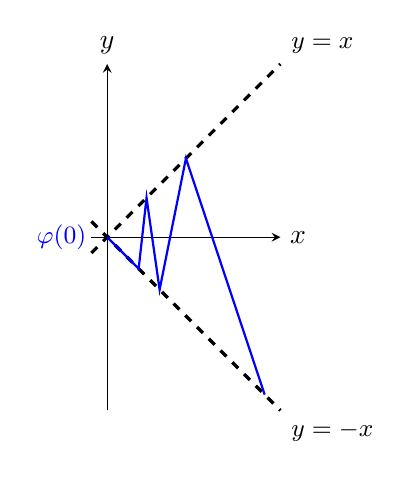
\begin{tikzpicture}[scale=2,>=stealth]
      % assi cartesiani senza tick labels
      \draw[->] (-0.1,0) -- (1.1,0) node[right] {$x$};
      \draw[->] (0,-1.1) -- (0,1.1) node[above] {$y$};
  
      % bisettrici in evidenza
      \draw[dashed,very thick,black] (-0.1,-0.1) -- (1.1,1.1) node[above right] {\small $y=x$};
      \draw[dashed,very thick,black] (-0.1,0.1) -- (1.1,-1.1) node[below right] {\small $y=-x$};
  
      % pochi rimbalzi della curva phi
      \draw[thick, blue]
        (1.000,-1.000) --
        (0.500, 0.500) --
        (0.333,-0.333) --
        (0.250, 0.250) --
        (0.200,-0.200) --
        (0,0);
  
      % etichetta della funzione a sinistra dell'origine
      \node[blue,left=4pt] at (0,0) {\small $\varphi(0)$};
    \end{tikzpicture}
  \end{center}

\pagebreak

\section{20 maggio}

\sproposition{Curva parametrica in forma polare}{
    Se la curva è data in forma polare come
    \(\rho(\theta)\) per \(\theta \in [0,2\pi]\)
    vale
    \[
        \varphi(\theta) = (\rho(\theta)\cos\theta, \rho(\theta)\sin\theta)
    \]
    quindi assumendo che sia differenziabile
    \[
        \varphi' = (\rho'(\theta)\cos\theta - \rho(\theta) \sin\theta, \rho'(\theta)\sin\theta + \rho(\theta)\cos\theta)
    \]
    Allora la norma è data da
    \begin{align*}
        ||\varphi'|| =
        {\left(
            (\rho^2)'(\theta) + \rho^2(\theta)
        \right)}^{1/2}
    \end{align*}
}

\sexercise{}{
    Consideriamo la curva \(\rho(\theta) = e^{-\theta}\)
    con \(\theta \in [0, \lambda]\).
    La sua lunghezza è data da
    \begin{align*}
        \integral[0][\lambda][{\left(e^{-2\theta} + e^{-2\theta}\right)}^{1/2}][\theta] 
        &= \sqrt{2} \integral[0][\lambda][e^{-\theta}][\theta] \\
        &= \sqrt{2} \left(1 - e^{-\lambda}\right)
    \end{align*}
    Chiaramente la lunghezza tende a \(\sqrt{2}\), cioè quando la spirale
    tende verso l'origine.
}

\sexercise{}{
    Calcolare la lunghezza di
    \(y=x^2\) con \(x\in [0,1]\).
}

\pagebreak

\subsection{Differenziali}

\sdefinition{Spazio duale di \({\mathbb{R}^n}\)}{
    Lo spazio \(\left(\mathbb{R}^n\right)'\)
    è lo \emph{spazio duale} di \(\mathbb{R}^n\),
    ossia l'insieme dei funzionali lineare da \(\mathbb{R}^n\)
    a \(\mathbb{R}\).
}

Chiaramente tutti i funzionali lineari di tali spazio sono un caso particolare
delle matrici, cioè vettori. Ogni tale funzionale può essere scritta come
\begin{align*}
    f(x) &= (x,y), \quad y\in \mathbb{R}^n \\
    &= \sum x_i y_i
\end{align*}
che è il prodotto interno fra due vettori di \(\mathbb{R}^n\).
In particolare, in tale spazio vi è
\[
    \text{d}x_i \in \left(\mathbb{R}^n\right)'
\]
definita da
\[
    \text{d}x_i(x) \triangleq x_i = (x, e_i)
\]
ossia un operatore che mi restituisce la componente \(i\)-esima.
Tale operatore è equivalente alla moltiplicazione per il vettore della base
canonina della coordinata \(i\).
Tali funzionali rappresentano una base dello spazio duale, che è a sua volta uno spazio vettoriale.
Quindi ogni funzionale lineare può essere espresso come
\[
    f = \sum_{i=1}^n \alpha_i \,\text{d}x_i
\]

\sdefinition{Forma differenziale}{
    Sia \(\Omega \subseteq \mathbb{R}^n\).
    Allora una funzione \(\omega \colon \Omega \to (\mathbb{R})'\)
    che è continua è detta \emph{forma differenziale lineare}.
}

Rappresentiamo un differenziale
\[
    \omega(x) = \sum_{i=1}^n \alpha_i(x) \,\text{d}x_i
\]
dove \(\alpha_i \colon \Omega \to \mathbb{R}\) che devono essere continue.

\sexample{Forma differenziale}{
    La funzione
    \[
        \omega(x,y,z) = x^2\text{d}x - e^z \text{d}y + (xyz)\text{d}z
    \]
    è una forma differenziale da \(\mathbb{R}^3\) a \((\mathbb{R}^3)'\).
    La forma differenziale calcola in un punto mi restituisce un funzionale lineare.
    \[
        \omega(1,1,0) = \text{d}x - \text{d}y
    \]
    Tale funzionale, applicato ad un vettore diventa
    \[
        \omega(1,1,0)(\alpha, \beta, \gamma) = \alpha - \beta
    \]
    è equivalente all'oggetto \((x^2, -e^z, xyz)\), che è anche un campo vettoriale.
    Infatti, nel punto \((1,1,0)\) il campo vettoriale ha \((1, -1, 0)\).
}

\pagebreak

\sexample{Forme differenziali indotte da funzioni differenziabili}{
    Possiamo ottenere una forma differenziale prendendo una funzione
    \(F \colon \Omega \to \mathbb{R}\) che sia differenziabile.
    Allora il differenziale \(\text{dF}\) è una forma lineare.
    Questo funzionale lineare è rappresentato dal gradiente
    \[
        \text{dF} \equiv
        \left(
            \frac{\partial F}{\partial x_1},
            \cdots,
            \frac{\partial F}{\partial x_n}
        \right)
    \]
    quindi
    \begin{align*}
        \omega(x) = \sum_{i=1}^n
        \frac{\partial F}{\partial x_i}(x) \,\text{d}x_i
    \end{align*}
}

Per esempio sia \(F(x,y) = x^2y + \ln x\)
per \(\Omega = \{ x>0\}\).
Allora \(\omega(x,y) = (2xy + 1/x)\text{d}x +x^2\text{d}y\).

\sdefinition{Differenziale esatto}{
    Una forma differenziale \(\omega \colon \Omega \to (\mathbb{R}^n)'\)
    è detta \emph{esatta} se esiste una funzione
    \(F \colon \Omega \to \mathbb{R}\) differenziabile
    tale che \(\omega = \text{d} F\).
    Una tale funzione \(F\) viene detta \emph{primitiva} di \(\omega\).
}

Chiaramente \(F + C\) con \(C\) costante è ancora una primitiva.
Se due funzioni hanno la medesima derivata, allora le funzioni
non differiscono necessariamente di una costante - solo se sono
definite su insiemi connessi.
Per esempio
\[
    f(x) = \begin{cases}
        1 & x\in [0,1] \\
        0 & x\in[3,4]
    \end{cases}
\]
gli insiemi connessi in \(\mathbb{R}\) sono solo gli intervalli.
In \(\mathbb{R}^n\) al posto degli intervalli usiamo gli insiemi connessi.

\sdefinition{Insieme connesso}{
    Un insieme aperto \(\Omega\) è connesso se
    \[
        \Omega = A \cup B
    \]
    con \(A,B\) aperti, disgiunti, allora \(A\) o \(B\) è vuoto.
}

\sproposition{}{
    Sia \(F\colon \Omega \to \mathbb{R}\) differenziabile
    e \(\Omega\) connesso.
    Se \(\text{d}F = 0\), allora \(F\) è costante in \(\Omega\).
}

\sdefinition{Integrale su curva}{
    Consideriamo \(\omega \colon \Omega \to (\mathbb{R}^n)'\)
    e una curva \(\varphi \colon [a,b] \to \Omega\) regolare.
    Allora
    \[
        \int_\varphi \omega \triangleq \integral[a][b][
            \sum_{i=1}^n \alpha_i(\varphi(t)) \varphi_i'(t)
        ][t]
    \]
}
Chiaramente \(\alpha_i(\varphi(t))\) è un prodotto interno.
È come se la forma differenziale agisse sulla derivata
(sul vettore delle derivate).

\sexample{}{
    Supponiamo che
    \[
        \varphi(t) = (t,t^2), \quad t\in[0,1]
    \]
    e
    \[
        \omega(x,y) = y\text{d}x - xy\text{d}y
    \]
    Allora \(\)
    \begin{align*}
        \int_\varphi \omega
        &= \integral[0][1][
            (t^2 - t\cdot t^3)
            \cdot \varphi'(t)
        ][t] \\
        &= \integral[0][1][
            (t^2  - t\cdot t^3)
            \cdot (1,2t)
        ][t] \\
        &= \integral[0][1][
            t^2 \cdot 1 - t^3(2t)
        ][t]
    \end{align*}
}

\sexample{Integrale con forma differenziale esatta}{
    \begin{align*}
        \int_\varphi \text{d}F
        &= \integral[a][b][
            \sum_{j=1}^m
            \frac{\partial F}{\partial x_i}(\varphi(t))
            \varphi'_j(t)
        ][t]
    \end{align*}
}

Consideriamo \(H(t) = F(\varphi(t))\)
funzione composta

\begin{center}
% https://tikzcd.yichuanshen.de/#N4Igdg9gJgpgziAXAbVABwnAlgFyxMJZABgBpiBdUkANwEMAbAVxiRGTtICMKQBfUuky58hFAEZyVWoxZsAOvIDyAWxgBzOv0EgM2PASIAmKdXrNWiEIpV0cACy5dgAJT79pMKOvhFQAMwAnCBUkMhAcCCRJEC4YMCgkAGZw8zkrRXpAtHssbQDg0MQYyKQTWPjExBTqBjo4hgAFYQMxEAYYfxwQM1lLEAAxfJAgkLDqUsRyuISkAFoa9vqYJpbRNkCsdXtu3os2AAkPPiA
\begin{tikzcd}
{[a,b]} \arrow[r, "\varphi", bend left] \arrow[rr, "H"', bend right] & \Omega \arrow[r, "F", bend left] & \mathbb{R}
\end{tikzcd}
\end{center}

allora
\begin{align*}
    H'(t) &=
    \left(
        \frac{\partial F}{\partial x_i}(\varphi(t)),
        \cdots,
        \frac{\partial F}{\partial x_i}(\varphi(t)),
    \right)
    \begin{pmatrix}
        \varphi_1'(t) \\ \cdots \\ \varphi_n'(t)
    \end{pmatrix} \\
    &= \integral[a][b][H'(t)][t] = H(b) - H(a)
\end{align*}
Quindi,
\[
    \int_\varphi \text{d}F = F(\varphi(b)) - F(\varphi(a))
\]
Quindi quando la forma differenziale è esatta, tale integrale
è esattamente la differenza di \(F\) fra il punto finale e quello iniziale
della curva, quindi non dipende dal percorso.

\sproposition{Proprietà}{
    \begin{enumerate}
        \item \emph{linearità}
        \[
            \int_\varphi (\alpha\omega_1 + \beta\omega_2)
            = \alpha\int_\varphi \omega_1
            + \beta\int_\varphi \omega_2
        \]
        \item questo integrale è anch'esso un funzionale lineare
        definito sull'insieme delle forme differenziali.
        \item se \(\tilde{\varphi} = \varphi\), cioè \(\varphi(t) = \varphi(\sigma(t))\),
        allora
        \[
            \int_{\tilde{\varphi}} = \pm \int_{\varphi} \omega
        \]
        dove \(\pm\) è il segno di \(\sigma'\). Infatti
        \begin{align*}
            \int_{\tilde{\varphi}} \omega &=
            \integral[a][b][
                \sum_{j=1}^n \alpha_j (\tilde{\varphi}(t))
                \hat{\varphi}_j'(t)
            ][t] \\
            &= \integral[a][b][
                \sum_{j=1}^n \alpha_j
                (\varphi(\sigma(t)))\varphi_j'(\sigma(t))
                \sigma'(t)
            ][t] \\
            &=
            \integral[c \text{ o } d][d\text{ o } c][
                \sum_{j=1}^n \alpha_i (\varphi(s))\varphi_j'(s)
            ][s]
            \quad s = \sigma(t) \\
            &= \pm \int_\varphi\omega
        \end{align*}
        quindi a seconda del segno della derivata di omega otteniamo
        il verso di integrazione.
        \item siano \(\varphi_i \colon [a,b] \to \mathbb{R}^n\)
        e \(\varphi_2 \colon [c,d] \to \mathbb{R}^n\)
        tale che \(\varphi_1(b) = \varphi_2(c)\).
        Allora definiamo \(\varphi_1 \cup \varphi_2 \colon I \to \mathbb{R}\)
        con \(I\) intervallo siccome l'intervallo posso sceglierlo a piacimento
        a meno di curve equivalenti. Allora
        \[
            \int_{\varphi_1 \cup \varphi_2} \omega =
            \int_{\varphi_1} \omega +
            \int_{\varphi_2} \omega
        \]
        Queste unioni sono curve regolari a tratti.
    \end{enumerate}
}

\sdefinition{Insieme connesso per archi}{
    Un sottoinsieme \(\Omega \subseteq \mathbb{R}^n\) aperto è detto
    \emph{connesso per archi} se \(\forall p, q \in \Omega\),
    esiste una curva regolare a tratti
    \(\varphi\colon [a,b] \to \Omega\)
    tale che \(\varphi(a) = p \land \varphi(b) = q\).
}

\stheorem{}{
    Un insieme \(\Omega \subseteq \mathbb{R}^n\)
    è connesso per archi se e solo se è connesso.
}

\stheorem{}{
    Sia \(\Omega\) un insieme connesso e \(\omega\)
    una forma differenziale in \(\Omega\).
    Se \(\forall p, q \in \Omega\),
    \[
        \int_{\varphi_1} \omega = \int_{\varphi_2} \omega
    \]
    per ogni \(\varphi_1, \varphi_2 \to \Omega\)
    tali che \(\varphi_1(a) = \varphi_2(c) = p\)
    e \(\varphi_1(b) = \varphi_2(d) = q\),
    allora \(\omega\) è esatta.
}

Quindi vale anche il converso - se l'integrale dipende solo dal punto
iniziale e dal punto finale, allora il differenziale è esatto.

\sproof{}{
    Sia \[S_{p,q} = \left\{\varphi\colon I \to \Omega \,|\, \varphi(a) = p \land \varphi(b) = q\right\}\]
    Fissiamo \(p\) e prendiamo \(x\in\Omega\) e sia \(\varphi \in S_{p,x}\).
    Allora coincidono
    \begin{align*}
        F(x) = \int_\varphi \omega
    \end{align*}
    Mostriamo che \(F\) è la primitiva.
    Partiamo dal punto \(x\) e prendiamo un versore \(v\),
    quindi giungiamo ad un punto \(x + vh\) per qualche \(h\) (sempre rimanente dell'insieme).
    Allora, chiamando tale segmento \(r\)
    \begin{align*}
        F(x + vh) - F(x) &=
        \int_{\varphi \cup r} \omega - \int_\varphi \omega \\
        &= \int_r \omega
    \end{align*}
    Parametrizziamo quest'ultimo in qualsiasi modo, per esempio
    \begin{align*}
        \int_r \omega
        &= \integral[b][b+1][
            \sum_{j=1}^n \alpha_j(r(t)) r_j'(t)
        ][t] \\
        &= \integral[b][b+1][
            \sum_{j=1}^n \alpha_j(x + hv(t-b))v_j h
        ][t] \\
        &= \integral[0][h][
            \sum_{j=1}^n \alpha_j (x + vs)v_j
        ][s]
    \end{align*}
    dove abbiamo usato \(s = h(t-b)\).
    Abbiamo allora la derivata direzionale di \(F\)
    \begin{align*}
        \frac{F(x + hv) - F(x)}{h}
        &= \frac{1}{h} \integral[0][h][
            \sum_{j=1}^n \alpha_j (x + vs)v_j
        ][s] \\
        &= \frac{h}{h} \sum_{j=1}^n \alpha_k (x + vc)v_j
    \end{align*}
    per il teorema del valor medio con qualche \(c \in (0,h)\).
    Quando \(h\to 0\), \(c\to 0\), e siccome la funzione è continua
    vale il secondo limite, e quindi anche la derivata direzionale
    \begin{align*}
        \frac{\partial F}{\partial v}(x)
        &= \sum_{j=1}^n \alpha_j(x) v_j \\
        \frac{\partial F}{\partial x_k}(x) &= \alpha_k (x)
    \end{align*}
    in quanto per tale direzione rimane solo la coordinata \(k\)-esima.
}

Quindi tale funzione è una primitiva, e tutte le primitive differiscono per costante.

\scorollary{}{
    Con le stesse ipotesi di prima. Allora \(\omega\) è esatta se e solo se
    \[
        \int_\varphi \omega = 0
    \]
    per ogni curva regolare chiusa \(\varphi\) in \(\Omega\).
}

Prendendo due punti \(p, q\) possiamo considerare due cammini da \(p\) a \(q\).
Uno dei due cammini, lo riparametrizziamo in senso opposto, in maniera tale da ottenere
un cammino chiuso.
\begin{align*}
    0 = \int_{\varphi_1 \cup \varphi_2} \omega
    &= \int_{\varphi_1} \omega - \int_{\varphi_2}
\end{align*}
quindi i due integrali sono uguali.
Quindi, per mostrare che una forma differenziale è esatta possiamo
mostrare che il suo integrale su ogni cammino chiuso è nullo.

Supponiamo ora di avere una forma differenziale esatta \(\omega \in \mathcal{C}^1(\Omega)\),
quindi tutte le componenti \(\alpha_j \colon \Omega \to \mathbb{R}\)
sono di classe \(\mathcal{C}^1(\Omega)\), quindi tutte le derivate parziali sono di tale classe.
\[
    \frac{\partial F}{\partial x_k}(x) = \alpha_k(x) \qquad (\text{d}F = \omega)
\]
ma siccome hanno le derivate continue
\[
    \frac{\partial^2 F}{\partial x_k \partial x_j}(x)
    =
    \frac{\partial^2 F}{\partial x_j \partial x_k}(x)
\]
ma quindi
\[
    \frac{\partial \alpha_k}{\partial x_j} =
    \frac{\partial \alpha_j}{\partial x_k}
\]
per ogni \(j\) e \(k\).

\sexample{}{
    Sia \(\omega = X\text{d}x + Y\text{d}y\). Se la forma differenziale è esatta e della classe \(\mathcal{C}^1\)
    allora
    \[
        \frac{\partial X}{\partial Y}(x,y)
        = \frac{\partial Y}{\partial X}(x,y)
    \]
}

\sdefinition{Forma differenziale chiusa}{
    Sia \(\omega \in \mathcal{C}^1(\Omega)\) tale che
    \[
        \frac{\partial \alpha_k}{\partial x_j} =
        \frac{\partial \alpha_j}{\partial x_k}, \quad \forall x\forall i,j
    \]
    allora la forma è detta \emph{chiusa}.
}

Quindi ogni forma esatta è anche chiusa. Il converso non è vero

\sexample{}{
    Sia
    \[
        \omega = - \frac{y}{x^2 + y^2}\text{d}x + \frac{x}{x^2 + y^2}\text{d}y
    \]
    con \(\Omega = \mathbb{R}^2 \backslash \{(0,0)\}\).
    Allora
    \[
        \frac{\partial X}{\partial y} = \frac{y^2 - x^2}{{(x^2 + y^2)}^2}
    \]
    e
    \[
        \frac{\partial Y}{\partial x} = \frac{y^2 - x^2}{{(x^2 + y^2)}^2}
    \]
    quindi \(\omega\) è chiusa. Tuttavia, prendiamo ora \(\varphi(\theta) = (\cos\theta,\sin\theta)\)
    con \(\theta \in [0, 2\pi]\). Calcoliamo ora
    \begin{align*}
        \int_\varphi \omega = \integral[0][2\pi][
            \left(
                \frac{\sin^2\theta}{\cos^2\theta + \sin^2\theta}
                + \frac{\cos^2\theta}{\cos^2\theta + \sin^2\theta}
            \right)
        ][\theta] = 2\pi \neq 0
    \end{align*}
    quindi non è esatta.
}

\sdefinition{Insiemi stellati}{
    Sono sottoinsiemi \(\Omega \subseteq \mathbb{R}^n\) dove
    \[
        \exists \overline{x} \in \Omega \,|\,
        \forall x \in \Omega, [\overline{x}, x] \subseteq \Omega
    \]
    dove \([\overline{x}, x]\) è un segmento.
}

Ogni insieme convesso è stellato, in quanto è una condizione più forte.

\stheorem{}{
    Sia \(\omega\colon \Omega \to (\mathbb{R})'\) in \(\mathcal{C}^1(\Omega)\)
    e \(\Omega\) sia stellato. Se \(\omega\) è chiusa, allora è esatta.
}

\sproposition{}{
    Sia \(f\colon [a,b] \times A\) con \(A \subseteq \mathbb{R}^n\) aperto
    tale che \(f \in \mathcal{C}^1([a,b] \times A)\).
    Allora, \[
        F(x) = \integral[a][b][f(t,x)][t] \in \mathcal{C}^1(A)
    \]
    e
    \[
        \frac{\partial F}{\partial x_k} = \integral[a][b][
            \frac{\partial f}{\partial x_k}(t,x)
        ][t]
    \]
}

\sproof{Del teorema}{
    Siccome \(\Omega\) è stellato, esiste \(\overline{x}\)
    tale che la condizione di stellarità è soddisfatta, e
    \[
        \varphi(t) = \overline{x} + (x-\overline{x})t, \quad t\in[0,1]
    \]
    dove \(\varphi\colon [0,1] \to \Omega\), che quindi unisce i punti.
    Abbiamo allora
    \begin{align*}
        F(x) &= \int_\varphi \omega \\
        &= \integral[0][1][
            \sum_{j=1}^n \alpha_j (\overline{x} + (x-\overline{x})t) (x_j - \overline{x_j})
        ][t] \\
        \frac{\partial F}{\partial x_k}(x) &=
        \integral[0][1][
            \frac{\partial \alpha_j}{\partial x_k}
            \left(
                \sum_{j=1}^n \alpha_j (\overline{x} + (x-\overline{x})t) (x_j - \overline{x_j})
            \right)
        ][t] \\
        &= \integral[0][1][
            \sum_{j=1}^n \left(\frac{\partial \alpha_j}{\partial x_k}
            \left(
                \alpha_j (\overline{x} + (x-\overline{x})t) (x_j - \overline{x_j})
            \right)\right)
        ][t] \\
        &= \integral[0][1][
            \sum_{j=1}^n \left(\frac{\partial \alpha_j}{\partial x_k}
            \left(
                %\frac{\partial \alpha_j}{\partial x_k}
                (\overline{x} + (x-\overline{x})t)t(x_j - \overline{x_j})
            \right)\right)
        ][t] \\
        &= \integral[0][1][
            \sum_{j=1}^n
            \frac{\partial \alpha_j}{\partial x_k}
            (\overline{x} + (x-\overline{x})t)t(x_j - \overline{x_j})
            + \alpha_k(\overline{x} + (x-\overline{x})t)
        ][t] \\
        &= \integral[0][1][
            \sum_{j=1}^n
            \frac{\partial \alpha_k}{\partial x_j}
            (\overline{x} + (x-\overline{x})t)t(x_j - \overline{x_j})
            + \alpha_k(\overline{x} + (x-\overline{x})t)
        ][t] \\
        &= \integral[0][1][
            \frac{d}{dt} \left(t\alpha_k (\overline{x} + (x-\overline{x})t)\right)
        ][t] \\
        &= \left[t\alpha_k (\overline{x} + (x-\overline{x})t)\right]^1_0 \\
        &= \alpha_k(x)
    \end{align*}
    quindi la forma differenziale è esatta.
}

\sexample{}{
    Consideriamo
    \[
        \omega = (y^2 + y\cos z)\text{d}x +
        (2xy + x\cos z)\text{d}y +
        (x - xy \sin z)\text{d}z
        = X\text{d}x + Y\text{d}y + Z\text{d}z
    \]
    e la curva \(\varphi(t) = (t^3, t^2, t)\) con \(t \in [0,\pi]\).
    Vogliamo calcolare
    \[
        \int_\varphi \omega
    \]
    Cominciamo verificando se \(\omega\) è chiusa. Abbiamo
    \begin{align*}
        \frac{\partial X}{\partial y} &= 2y + \cos z \\
        \frac{\partial X}{\partial z} &= -y\sin z \\
        \frac{\partial Y}{\partial x} &= 2y + \cos z \\
        \frac{\partial Y}{\partial z} &= -x\sin z \\
        \frac{\partial Z}{\partial x} &= 1-y\sin z \\
        \frac{\partial Z}{\partial y} &= -x\sin z
    \end{align*}
    per colpa di quell'1 non è chiusa, e quindi non è esatta. Tuttavia, spezziamo
    la forma come
    \(\omega = \omega_1 + \omega_2\)
    con
    \[
        \omega_1 = (y^2 + y\cos z)\text{d}x +
        (2xy + x\cos z)\text{d}y +
        (- xy \sin z)\text{d}z
    \]
    e
    \[
        \omega_2 = x\text{d}z
    \]
    Allora \(\omega_1\) è chiusa (e quindi esatta siccome l'insieme è puntato).
    Abbiamo quindi
    \begin{align*}
        \int_\varphi \omega &= \int_\varphi \omega_1 + \int_\varphi \omega_2
    \end{align*}
    Il secondo integrale è dato da
    \[
        \integral[0][\pi][t^3][t]
    \]
    Per il primo, visto che la forma è esatta, ci basta trovare una primitiva
    \[
        \frac{\partial F}{\partial x}(x,y,z) = X(x,y,z) = y^2 + y\cos z
    \]
    quindi integrando troviamo
    \[
        F(x,y,z) = xy^2 + xy\cos z + h(y,z)
    \]
    Analogamente
    \[
        \frac{\partial F}{\partial y} = Y(x,y,z) = 2xy + x\cos z + \frac{\partial h}{\partial y}(y,z)
    \]
    ma per confronto
    \[
        \frac{\partial h}{\partial y}(y,z) = 0
    \]
    quindi
    \[
        h(x,z) = C + k(z)
    \]
    Allora,
    \[
        \frac{\partial F}{\partial z} = -xy\sin z + k'(z) = -xy\sin z
    \]
    e allora 
    \[
        k'(z) = 0
    \]
    cioè \(k = C\). Quindi,
    \[
        F(x,y,z) = xy^2 + xy\cos z
    \]
    dove abbiamo preso costante nulla.
    In conclusione,
    \begin{align*}
        \int_\varphi \omega_1 = F(\pi^3, \pi^2, \pi) - F(0,0,0)
    \end{align*}
}

Quando calcoliamo un integrale su forma esatta possiamo classicamente prendere un cammino
lineare che congiunge i due punti oppure un cammino a segmenti per ogni componente.

\sproposition{}{
    Supponiamo ora di avere una equazione differenziale del tipo
    \[
        y' = \frac{X(x,y)}{Y(x,y)}
    \]
    e supponiamo di avere la forma differenziale esatta
    \[
        \omega = X\,dx - Y\,dy
    \]
    siccome è esatta esiste il potenziale \(F\).
    Supponiamo anche che esiste una funzione \(y(x)\) tale che
    \[
        \forall x\in I \, F(x, y(x)) = 0
    \]
    su qualche intervallo.
    Allora
    \begin{align*}
        y'(x) &= - \frac{
            \frac{\partial F}{\partial x}(x,y(x))
        }{
            \frac{\partial F}{\partial y}(x,y(x))
        } \\
        &= - \frac{X(x,y(x))}{Y(x,y(x))}
    \end{align*}
    quindi la funzione esplicita descritta da \(F = 0\) è una soluzione dell'equazione differenziale.

    Possiamo anche scegliere di moltiplicare per un fattore integrante
    \[
        y'(x) = \frac{CX(x,y)}{CY(x,y)}
    \]
    che sia per esempio \(C = C(y)\). La forma associata è
    \[
        \omega = CX\,dx - CY\,dy
    \]
    che è esatta se
    \begin{align*}
        \frac{\partial X}{\partial y}C + CX &= C \frac{\partial Y}{\partial y} \\
        C' &= -C \left(
            \frac{\frac{\partial X}{\partial y} + \frac{\partial Y}{\partial x}}{X}
        \right)
    \end{align*}
    Possiamo anche scegliere \(C = C(x)\), la forma è esatta se
    \begin{align*}
        \frac{\partial (XC)}{\partial y} &= -\frac{\partial (YC)}{\partial X} \\
        \frac{\partial X}{\partial y}C = -\frac{\partial Y}{\partial x} C - YC'
    \end{align*}
    quindi abbiamo
    \[
        C' = -C \left(
            \frac{\frac{\partial X}{\partial y} + \frac{\partial Y}{\partial x}}{Y}
        \right)
    \]
    se dipende solo da \(x\) possiamo quindi risolvere l'equazione in tale modo.
    Nel caso in cui \(C=C(x,y)\) l'equazione dell'esattezza è una equazione differenziale parziale.
}

\pagebreak

\section{Esercizi}

\subsection{Convergenze serie e successioni}

% TODO gli esercizi di giacomo

% 25 gennaio 2018 tema d'esame
\sexercise{Successioni 1}{
    Per \(x > -1\) studia la successione
    \[
        f_n(x) = \frac{ne^{-n/x}}{x^2\sqrt{1 + x}}
    \]
    \begin{itemize}
        \item \textbf{convergenza puntuale:} controlliamo la convergenza puntuale in \(E = (0, +\infty)\).
        Fissato \(x > 0\) studiamo
        \begin{align*}
            \lim_n f_n(x) = \lim_n \frac{ne^{-n/x}}{x^2\sqrt{1 + x}} = 0 = f(x)
        \end{align*}
        \item \textbf{convergenza uniforme:} controlliamo la convergenza uniforme in \(E\).
        Abbiamo
        \begin{align*}
            {||f_n - f||}_{\infty, E} &= \sup_{x\in (0, +\infty)} \left|
                \frac{ne^{-n/x}}{x^2\sqrt{1 + x}}
            \right|
        \end{align*}
        sostituendo \(t = n/x\) otteniamo una funzione simile all'integranda della funzione gamma, che ha un massimo \(M\)
        \begin{align*}
            \sup_{x\in (0, +\infty)} \left|
                \frac{ne^{-n/x}}{x^2\sqrt{1 + x}}
            \right| &\leq M \sup_{x\in (0, +\infty)} \frac{1}{n\sqrt{1 + x}} \\
            &= \frac{M}{n \varepsilon} \to 0
        \end{align*}
        Chiaramente il sup si ottiene con il denominatore più piccolo, quindi un \(\varepsilon\) molto vicino a \(0\).
        \item \textbf{integrabilità:} mostriamo che \(f_n \in L^1\).
        \begin{align*}
            \integral[0][\infty][|f_n(x)|][x] &=
            \integral[0][\infty][\left|\frac{ne^{-n/x}}{x^2\sqrt{1 + x}}\right|][x] 
        \end{align*}
        In un intorno di \(+\infty\) abbiamo
        \[
            f_n(x) \sim \frac{n}{x^{5/2}}
        \]
        siccome \(\frac{5}{2}>1\) la funzione è integrabile a infinito.
        In un intorno di \(0^+\) maggioriamo
        \[
            f_n(x) \leq \frac{M}{n\sqrt{1 + x}} \sim \frac{M}{n}
        \]
        quindi è integrabile per confronto e confronto asintotico.
    \end{itemize}
}

\pagebreak

\sexercise{Successioni 1}{
    Data la successione
    \[
        f_n(x) = n^\alpha \arctan(x)e^{n^2 x}
    \]
    studiare al variare di \(\alpha\in\mathbb{R}\)
    \begin{enumerate}
        \item \textbf{convergenza puntuale:} studiamo la convergenza puntuale in \((0, +\infty)\).
        Fissato \(x>0\) abbiamo
        \begin{align*}
            \lim_n f_n(x) &= \lim_n n^\alpha \arctan(x)e^{n^2 x} = 0, \forall \alpha \in \mathbb{R}
        \end{align*}
        \item \textbf{convergenza uniforme:} studiamo la convergenza uniforme in \((0, +\infty)\).
        Abbiamo
        \begin{align*}
            {||f_n - f||}_{\infty, E} &= \sup_{x\in (0, +\infty)} \left|
                n^\alpha \arctan(x)e^{n^2 x}
            \right| \\
            &\leq \sup_{x\in (0, +\infty)} \left|
                n^\alpha x e^{n^2 x}
            \right|
        \end{align*}
        siccome \(\arctan(x) \leq x\). Studiamo la derivata della funzione maggiorante \(g_n(x)\).
        \begin{align*}
            g_n'(x) &= n^\alpha e^{-n^2x} - n^\alpha x e^{-n^2 x} n^2 \\
            &= n^\alpha e^{-n^2 x}(1-xn^2)
        \end{align*}
        Per studiare il segno abbiamo
        \begin{align*}
            1 - n^2 x \leq 0 \iff x \leq \frac{1}{n^2}
        \end{align*}
        che è un punto di massimo. Chiaramente \(g_n(0)=0\) e \(\lim_{x\to\infty} g_n(x)\),
        e siccome è sempre positiva, siamo sicuri che tale valore è un punto di massimo.
        Il massimo vale
        \[
            g_n\left(\frac{1}{n^2}\right) = \frac{n^{\alpha-2}}{e}
        \]
        Quindi, la norma infinito è sempre minore di 
        \begin{align*}
            ||f_n-f||_{\infty, E} &\leq \frac{n^{\alpha-2}}{e}
        \end{align*}
        che tende a zero solo quando \(\alpha < 2\) (condizione sufficiente ma non necessaria).
    Cerchiamo ora un limite dal basso
    \begin{align*}
        ||f_n-f||_{\infty, E} \geq f_n\left(\frac{1}{n^2}\right)
        &= n^\alpha \arctan\left(\frac{1}{n^2}\right)e^{-1} \\
        &\sim n^{\alpha - 2}e^{-1}
    \end{align*}
    che non tende a zero. Quindi la convergenza è uniforme per \(\alpha < 2\).
    \end{enumerate}
}

\pagebreak

% 2 sett 2020
\sexercise{Successioni 3}{
    Data la successione
    \[
        f_n(x) = n\left(e^{\frac{x^2}{n}} - 1\right)
    \]
    \begin{enumerate}
        \item \textbf{stabilire in che insieme vi è convergenza puntuale:} fissato \(x\) calcoliamo
        \begin{align*}
            \lim_n f_n &= \lim_n n\left(e^{\frac{x^2}{n}} - 1\right) = x^2
        \end{align*}
        in quanto la parentesi è asintotica all'esponente. Allora l'insieme di convergenza puntuale è \(E = \mathbb{R}\).
        \item \textbf{stabilire se la convergenza è uniforme in tale insieme:} fissato \(x\) abbiamo
        \begin{align*}
            {||f_n - f||}_{\infty, E} &= \sup_{x\in (0, +\infty)} \left|
                n\left(e^{\frac{x^2}{n}} - 1\right) - x^2
            \right| = \sup_{x\in (0, +\infty)} \left|
                g_n(x)
            \right|
        \end{align*}
        Studiamo la derivata di \(g_n(x)\)
        \[
            g_n'(x) = ne^{\frac{x^2}{n}}\frac{2x}{n} - 2x = 2x\left(
                e^{\frac{x^2}{n}} - 1
            \right)
        \]
        Il segno della derivata è lo stesso di \(x\), e \(x=0\) è un punto di minimo.
        \[
            \lim_{x\to\pm\infty} g_n(x) = \pm\infty
        \]
        quindi non è limitata e la convergenza non è assoluta.
        \item \textbf{stabilire se la convergenza è uniforme in un intervallo limitato:} sia \([a,b]\) tale intervallo.
        Dalla forma della funzione, il sup è o in \(x=a\) o in \(x=b\), quindi
        \begin{align*}
            ||f_n - f||_{\infty, E} \leq \max\{|f(a)-f(b)|, |f(b)-f(a)|\}
        \end{align*}
        supponiamo che sia in \(a\)
        \begin{align*}
            ||f_n - f||_{\infty, E} = \left|n\left(e^{\frac{a^2}{n}} - 1\right) - a^2\right|
        \end{align*}
        per risolvere il limite facciamo un espansione di MacLaurin fino al secondo ordine
        \begin{align*}
            ||f_n - f||_{\infty, E} = \left|
                \frac{a^4}{n} + o\left(\frac{1}{n}\right)
            \right| \to 0
        \end{align*}
        Quindi, la convergenza è uniforme in un intervallo limitato.
    \end{enumerate}
}

\pagebreak

\sexercise{Serie 1}{
    Consideriamo la serie
    \[
        \sum_{n=1}^\infty \frac{xe^{-\frac{x^2}{n}}}{n^2 + x^2}
    \]
    verifica la convergenza uniforme in \(\mathbb{R}\). Cominciamo studiando la convergenza totale
    che è più forte, quindi la convergenza di
    \begin{align*}
        \sum_{n=1}^\infty ||f_n||_{\infty, \mathbb{R}}
        &= \sum_{n=1}^\infty \sup_{x\in\mathbb{R}}
        \left|
            \frac{xe^{-\frac{x^2}{n}}}{n^2 + x^2}
        \right|
    \end{align*}
    con \(t = \frac{x}{\sqrt{n}}\) otteniamo la forma \(f(t)=te^{-t^2}\) che ha grafico noto,
    e un massimo \(M\) e minimo
    \begin{align*}
         ||f_n||_{\infty, \mathbb{R}}
        &\leq M \sup_{x\in\mathbb{R}}
        \frac{\sqrt{n}}{n^2 + x^2}
        = \frac{M}{n^{3/2}}
    \end{align*}
    in quanto il supremum è per \(x=0\). Quindi la serie
    \begin{align*}
        \sum_{n=1}^\infty ||f_n||_{\infty, \mathbb{R}}
        &\leq M \sum_{n=1}^\infty \frac{1}{n^{3/2}}
    \end{align*}
    che converge. Quindi la serie converge totalmente e quindi converge anche in maniera
    uniformemente su tutto \(\mathbb{R}\).
}

\sexercise{Serie 2}{
    Conderiamo la serie
    \[
        \sum_{n=1}^\infty \arctan\left(\frac{n^\alpha}{x^2 + n^2}\right)
    \]
    \begin{enumerate}
        \item Stabilire per quali \(\alpha \in \mathbb{R}\) abbiamo convergenza puntuale:
            Fissato \(x\), notiamo che per convergere il termine \(n\)-esimo deve tendere a zero.
            Quindi,
            \[
                \lim_n \arctan\left(\frac{n^\alpha}{x^2 + n^2}\right) \to 0
            \]
            se e solo se \(\alpha < 2\) (condizione necessaria).
            Usiamo il criterio del confronto asintotico: l'argomento dell'arcotangente tende a zero
            e quindi è asintotica al suo argomento.
            La serie
            \[
                \sum \frac{1}{n^{2 - \alpha}}
            \]
            converge se e solo se \(\alpha < 1\).
            Quindi, la serie converge puntualmente per \(\alpha < 1\).
        \item Stabilire per quali \(\alpha \in \mathbb{R}\) abbiamo convergenza uniforme:
        è necessario \(\alpha - 1\). Cominciamo studiando la convergenza totale, che è più forte.
        Abbiamo
        \begin{align*}
            \sum_{n=1}^\infty ||f_n||_{\infty, \mathbb{R}}
            &=\sum_{n=1}^\infty \sup_{x\in\mathbb{R}} \left|
                \arctan\left(\frac{n^\alpha}{x^2 + n^2}\right)
            \right|
        \end{align*}
        Studiamo la derivata del termine
        \begin{align*}
            f_n'(x) = \frac{1}{1 + {\left(\frac{n^\alpha}{x^2 + n^2}\right)}^2}
            &= - \frac{2xn^\alpha}{n^{2\alpha} + {n^2 + x^2}^2} \geq 0 \iff x \leq 0
        \end{align*}
        quindi \(x=0\) è un punto di massimo.
        Infatti, gli estremi sono
        \[
            \lim_{x\to\pm\infty} f_n(x) \to 0
        \]
        Quindi la forma è data da
        \[
            ||f_n||_{\infty, \mathbb{R}} = f_n(0) = \arctan(n^{\alpha - 2})
        \]
        La serie è quindi a termini positivi e usiamo il confronto asintotico
        \begin{align*}
            \sum_{n=1}^\infty ||f_n||_{\infty, \mathbb{R}} &=
            \sum_{n=1}^\infty \arctan(n^{\alpha - 2})
        \end{align*}
        che converge se e solo se \(\alpha < 1\). Quindi abbiamo convergenza uniforme
        per \(\alpha < 1\). Siccome la convergenza puntuale è per \(\alpha < 1\),
        non vi sono altri \(\alpha\) per cui vi è convergenza assoluta.
    \end{enumerate}
}

% tema esame 1 settembre 2022
\sexercise{Serie 3}{
    Consideriamo la serie
    \[
        \sum_{n=1}^\infty \frac{\arctan\left(\frac{x}{n^\alpha + 1}\right)}{\sqrt{n+1} - \sqrt{n}}
    \]
    \begin{enumerate}
        \item Valutare per quali \(\alpha\in\mathbb{R}\) vi è convergenza puntuale in \(\mathbb{R}\).
        Studiamo la condizione necessaria di convergenza.
        Il numeratore tende a zero se e solo se \(\alpha > 0\).
        In tal caso la funzione è assolutamente asintotica a
        \[
            |f_n(x)| \sim \frac{2|x|}{n^{\alpha - 1/2}}
        \]
        E la serie
        \[
            \sum_{n=1}^\infty \frac{2|x|}{n^{\alpha - 1 /2}}
        \]
        converge se e solo se \(\alpha > 3/2\) per confronto asintotico.
        Per \(x<0\), basta notare che \(\arctan(t)\) è simmetrica rispetto all'origine,
        il ché implica convergenza puntiale per \(\alpha > 3/2\).
        \item Stabilire per quali \(\alpha\in\mathbb{R}\) la somma della serie è continua in \(\mathbb{R}\).
        Dobbiamo utilizzare il teorema. Dobbiamo trovare per quali \(\alpha\) converge totale
        per applicare il teorema che dice che se \(f_n\) è continua in \(E\), allora la sua serie converge
        uniformemente a \(S(x)\) in \(E\) e \(S(x)\) è continua.
        Studiamo la convergenza totale in \(E = [-a, a]\), \(a>0\).
        Abbiamo allora
        \begin{align*}
            ||f_n||_{\infty, [-a, a]} &= \sup_{x\in[-a,a]}
            \frac{\arctan\left(\frac{x}{n^\alpha + 1}\right)}{\sqrt{n+1} - \sqrt{n}} \\
            &\leq \sup_{x\in[-a,a]} \frac{|x|}{n^\alpha + 1}2\sqrt{n}
            = \frac{2a\sqrt{n}}{n^{\alpha} + 1} \sim \frac{C}{n^{\alpha - 1/2}}
        \end{align*}
        in quanto \(\arctan(t) \leq t\).
        Ciò implica che
        \[
            \sum_{n=1}^\infty ||f_n||_{\infty, [-a, a]} \leq
            \sum_{n=1}^\infty \frac{C}{n^{\alpha - 1/2}}
        \]
        che converge se e solo se \(\alpha > 3/2\).
        Quindi per confronto la serie converge totalmente, e quindi uniformemente per \(\alpha > 3/2\).
        Poiché la convergenza uniforme implica la convergenza puntuale e la serie converge puntualmente
        per \(\alpha > 3/2\), abbiamo convergenza uniformemente se e solo se \(\alpha > 3/2\).
        Poiché \(f_n\) è continua e la serie converge uniformemente in \([-a, a]\), la serie risulta continua in tale intervallo.
        Poiché \(a\) è arbitrario, possiamo amplificato e la serie è continua su tutto \(\mathbb{R}\).
    \end{enumerate}
}

\subsection{Integrazione}

\sexercise{}{
    Sia 
    \[
        f_n(x) = \integral[x][x+n][\frac{\arctan t^2}{t^\alpha}][t]
    \]
    Studiamo la convergenza puntuale in \(x \in (0, \infty)\).
    Abbiamo problemi per \(t \to 0\) e \(t\to+\infty\).
    Nel limite abbiamo
    \begin{align*}
        \integral[x][\infty][\frac{\arctan t^2}{t^\alpha}][t]
    \end{align*}
    Il primo problema accade solo se \(0 \in [x, x+n]\).
    In infinito abbiamo
    \[
        \frac{\arctan t^2}{t^\alpha} \sim \frac{C}{t^\alpha}
    \]
    che è integrabile per \(\alpha > 1\). In un intorno di zero abbiamo
    \[
        \frac{\arctan t^2}{t^\alpha} \sim t^{2-\alpha}
    \]
    che è integrabile per \(\alpha < 3\).
    Quindi converge puntualmente per \(\alpha \in (1,3)\)
    Per guardare la convergenza uniforme abbiamo
    \begin{align*}
        \sup |f_n(x) - f(x)| &= \left|\,
            \integral[x][\infty][\frac{\arctan t^2}{t^\alpha}][t]
            - \integral[x][x + n][\frac{\arctan t^2}{t^\alpha}][t]
        \right|
        \\
        &= \left|\,
            \integral[x+n][\infty][\frac{\arctan t^2}{t^\alpha}][t]
        \right| \\
        &\leq \integral[x+n][\infty][\left|\frac{\arctan t^2}{t^\alpha}\right|][t] \\
        &= \integral[x+n][\infty][\frac{\arctan t^2}{t^\alpha}][t] \\
        &\leq \frac{\pi}{2} \integral[x+n][\infty][\frac{1}{t^\alpha}][t] \\
        &= \frac{\pi}{2} \frac{-{(x+n)}^{1-\alpha}}{1-\alpha} \to 0
    \end{align*}
    Abbiamo tolto il valore assolto perché l'intervallo è definitivamente positivo.
    La stima dell'errore è uniforme quindi la convergenza è uniforme.
    Studiamo ora per quali \(\alpha\), il limite di \(f_n\) è integrabile in \((0, +\infty)\).
    Osserviamo che \(f_n \geq 0\) e siccome l'intervallo di integrazione cresce, abbiamo che
    \(f_n \leq f_{n+1}\). Applichiamo allora il teorema della convergenza monotona, e
    \[
        \lim_n \integral[x][x+n][f_n][\mu] = \int f
    \]
    che è integrabile per \(\alpha \in (1,3)\).
}

\sexercise{}{
    Calcoliamo
    \[
        \lim_n \integral[0][+\infty][\frac{1 + x^{n+1}}{1 + x^n e^{2x}}][x]
    \]
    Abbiamo che
    \[
        f_n(x) \to \begin{cases}
            1 & 0<x<1 \\
            \frac{2}{1 + e^2} & x = 0 \\
            \frac{x}{e^{2x}} & x > 1
        \end{cases}
    \]
    Per \(0 < x \leq 1\)
    \[
        f_n(x) \leq 2
    \]
    che è integrabile nella parte limitata del dominio \((0, 1)\).
    Per \(x>1\) abbiamo
    \[
        f_n(x) \leq \frac{1 + x^{n+1}}{x^n e^{2x}}
        \leq \frac{2x^{n+1}}{x^n e^{2x}}
        = \frac{2x}{e^{2x}}
    \]
    Usiamo quindi la convergenza dominata
    \begin{align*}
        \lim_n \integral[0][+\infty][f_n][x]
        &= \integral[0][+\infty][\lim_n f_n(x)][x] \\
        &= \integral[0][1][1][x] + \integral[1][+\infty][\frac{x}{e^{2x}}][x] \\
        &= \frac{5}{4} + \frac{1}{2e}
    \end{align*}
}

% 25 gennaio 2022
\sexercise{}{
    Studiare l'integrabilità di
    \[
        f(x) = \frac{x^\alpha (1 - \cos^4(\pi x))}{\ln(x) \ln(1 + \sqrt{x})}
    \]
    in \((0, +\infty)\). Usiamo il confronto asintotico in un intorno di zero
    \begin{align*}
        f(x) \sim \frac{x^\alpha \cdot 4 \cdot \left(\frac{\pi^2x^2}{2}\right)}{
            \ln(x) \ln 2
        } = C \frac{x^{\alpha + 3/2}}{\ln x}
    \end{align*}
    che è integrabile per \(\alpha > -5/2\).
    Se \(x \to 1\) abbiamo
    \begin{align*}
        f(x) \sim \frac{4 \frac{{(x-1)}^2}{2}}{(x-1)\ln 2}
        = \frac{2}{\ln 2} (x-1)
    \end{align*}
    che è integrabile.
    Per \(x\to\infty\)
    \begin{align*}
        f(x) \leq \frac{2x^\alpha}{\ln x \ln(1 + \sqrt{x})}
        \sim 4 \frac{x^\alpha}{\ln^2(x)}
    \end{align*}
    che è integrabile per \(\alpha \leq 1\).
    Quindi, la funzione è integrabile per
    \[
        -\frac{5}{2} < x \leq -1
    \]
}

%\sexercise{}{
%    Considera
%    \[
%        F(x) = \integral[1][x][\frac{\ln(e^{xt} + 1)}{tx(t^2 + e^{1/x})}][t]
%    \]
%    Studia \(F(x)\) per \(x\to 0\). Prendiamo \(0<x<1\)
%    \begin{align*}
%        0 &\leq \integral[x][1][\frac{\ln(e^{xt} + 1)}{tx(t^2 + e^{1/x})}][t]
%        \leq \integral[x][1][\frac{1}{t^2 + e^{1/x}}][t] \\
%        &\leq \integral[x][1][\frac{1}{x^2 + e^{1/x}}][t]
%        \\
%        &= \frac{x-1}{x^2 + e^{1/x}} \to 0^+
%    \end{align*}
%}

\sexercise{}{
    Sia \(\alpha > 0\) e
    \[
        E\alpha = \left\{
            0<x<1 \land 1< y < x^{-\alpha}
        \right\}
    \]
    quindi
    \[
        |E_\alpha| = \integral[0][1][
            \integral[1][x^{-\alpha}][][y]
        ][x]
    \]
    che è finito se e solo se \(\alpha < 1\).
    Data \(f(x,y) = \arctan(x/y)\)
    calcolare
    \[
        \int_{E_\alpha} f(x,y)\,dx\,dy
    \]
    Possiamo applicare il teorema di Tonelli
    \begin{align*}
        \int_{E_\alpha} f(x,y)\,dx\,dy
        &= \integral[1][\infty][
            \integral[0][y^{-1/\alpha}][\arctan(x/y)][x]
        ][y] \\
        &= \integral[1][\infty][
            \integral[0][y^{-1/\alpha - 1}][\arctan(z)y][z]
        ][x] \\
        &= \integral[1][+\infty][
            y\left(
                y^{-1/\alpha - 1} \arctan\left(y^{-1/\alpha - 1}\right)
                - \frac{1}{2} \ln\left(y^{-2/\alpha - 2} + 1\right)
            \right)
        ][y]
    \end{align*}
    dove abbiamo sostituito \(z=x/y\).
    Per \(y\to\infty\), il primo termine
    \[
        y^{-1/\alpha}\arctan\left(y^{-1/\alpha - 1}\right)
        \sim y^{-1/\alpha} y^{-1/\alpha - 1}
        = y^{-1-2/\alpha}
    \]
    che è integrabile per \(\alpha > 0\).
    Per il secondo termine abbiamo
    \[
        y\frac{1}{2} \ln\left(y^{-2/\alpha - 2} + 1\right)
        \sim y^{-2/\alpha - 1}
    \]
    che è integrabile per ogni \(\alpha > 0\).
    Quindi \(f\) è integrabile per \(\alpha > 0\).
}

\pagebreak

\sexercise{}{
    Studiare l'integrabilità di
    \[
        f(x,y,z) = \frac{\arctan(z)}{{(x^2+y^2)}^\alpha}
    \]
    nell'insieme
    \[
        E = \{(x,y,z) \in \mathbb{R}^3 \,|\, 0<z<x^2 + y^2 <1\}
    \]
    al variare di \(\alpha \in \mathbb{R}\).
    Usiamo le coordinate cilindriche
    \[
        \begin{cases}
            x = \rho \cos\theta \\
            y = \rho \sin\theta \\
            z = z
        \end{cases}
    \]
    Il determinare della Jacobiana è \(\rho\). Abbiamo quindi la condizione
    \(0 < z < \rho^2\). Per la condizione su \(\rho\) notiamo che \(0 < \rho^2 < 1\)
    se e solo se \(0 < \rho < 1\). L'integrale diventa
    \begin{align*}
        \integral[0][2\pi][
            \integral[0][1][
                \integral[0][\rho^2][
                    \frac{\arctan(z)}{{(x^2+y^2)}^\alpha} \rho
                ][z]
            ][\rho]
        ][\theta]
        &= 2\pi \integral[0][1][
            \frac{1}{\rho^{2\alpha - 1}}
            \integral[0][\rho^2][\arctan z][z]
        ][\rho] \\
        &= 2\pi \integral[0][1][
            \frac{1}{\rho^{2\alpha - 1}} \left[
                \rho^2 \arctan \rho^2 - \frac{1}{2} \log(1 + z^2)
            \right]^{\rho^2}_0
        ][\rho] \\
        &= 2\pi
        \integral[0][1][
            \frac{\arctan \rho^2}{\rho^{2\alpha - 3}}
        ][\rho]
        - \pi \integral[0][1][
            \frac{\log(1 + \rho^4)}{\rho^{2\alpha - 1}}
        ][\rho]
    \end{align*}
    In un intorno di zero l'integranda del primo integrale è asintotica a
    \[
        \frac{\arctan \rho^2}{\rho^{2\alpha - 3}} \sim \frac{1}{\rho^{2\alpha - 5}}
    \]
    che è quindi integrabile se e solo se \(\alpha < 3\). Per la seconda integranda, la funzione è asintotica a
    \[
        \frac{\log(1 + \rho^4)}{\rho^{2\alpha - 1}} \sim \frac{1}{\rho^{2\alpha - 5}}
    \]
    che è come prima. Quindi.
    È importante notare che grazie alle costanti davanti agli integrali si evita cancellazione diretta.
    La funzione è integrabile per \(\alpha < 3\).
}

\pagebreak

\sexercise{}{
    Usando il cambio di variabili \(x = \sqrt{\rho \cos\theta}\) e \(y = \rho \sin\theta\)
    determinare per quali \(\alpha\in\mathbb{R}\) la funzione
    \[
        f(x,y) = \frac{x}{{(1 + x^4 + y^2)}^\alpha}
    \]
    è integrabile in \(\mathbb{R}^2\) e calcolare il valore di tale integrale.
    La funzione è dispari quindi ci restringiamo al primo quadrante. L'integrale è quindi zero dove esiste.
    Calcoliamo ora \(|\det J\varphi|\). Abbiamo
    \[
        \varphi \colon \begin{bmatrix} \rho \\ \theta \end{bmatrix} \to
        \begin{bmatrix} \sqrt{\rho\cos\theta} \\ \rho \sin\theta \end{bmatrix}
    \]
    Quindi
    \begin{align*}
        J\varphi = \begin{bmatrix}
            \frac{\partial x}{\partial \rho} && \frac{\partial x}{\partial \theta} \\
            \frac{\partial y}{\partial \rho} && \frac{\partial y}{\partial \theta} \\
        \end{bmatrix}
    \end{align*}
    il cui determinante è
    \[
        |\det J\varphi| = \frac{\rho\cos^2\theta}{2\sqrt{\rho\cos\theta}} +
        \frac{\rho\sin^2\theta}{2\sqrt{\rho\cos\theta}} = \frac{1}{2}\sqrt{\frac{\rho}{\cos\theta}}
    \]
    L'integrale diventa
    \begin{align*}
        &\phantom{=}\integral[0][\frac{\pi}{2}][
            \integral[0][\infty][
                \frac{\sqrt{\rho\cos\theta}}{{(1 + \rho^2\cos^2\theta + \rho^2\sin^2\theta)}^\alpha}
                \cdot  \frac{1}{2}\sqrt{\frac{\rho}{\cos\theta}}
            ][\rho]
        ][\theta] \\
        &= \frac{1}{2} \integral[0][\frac{\pi}{2}][
            \integral[0][\infty][
                \frac{\rho}{{(1 + \rho^2)}^\alpha}
            ][\rho]
        ][\theta]
    \end{align*}
    L'integrale esterno è indipendente e vale quindi \(\pi / 2\). Per l'integrazione
    abbiamo problemi in infinito, dove l'integranda è asintotica a
    \[
        \frac{\rho}{{(1 + \rho^2)}^\alpha} \sim \frac{1}{\rho^{2\alpha - 1}}
    \]
    che è integrabile per \(\alpha > 1\).
}

\pagebreak

\sexercise{}{
    Calcolare, giustificando la risposta
    \[
        \lim_{n} \int_{E_n} \log^2 \left(\frac{y}{x}\right)\,d\mu_2
    \]
    dove
    \[
        E_n = \left\{(x,y) \in \mathbb{R}^2 \,\middle|\, \frac{1}{n} < xy < 2 \land 1 < \frac{y}{x} < 2\right\}
    \]
    Notiamo che \(E_n \subseteq E_{n+1}\) e in termini di funzioni indicatrici \(\chi_{E_n} \leq \chi_{E_{n + 1}}\)
    che è quindi monotona crescente. Chiaramente
    \[
        \lim_n \chi_{E_n} = \chi_E
    \]
    dove
    \[
        E = \left\{(x,y) \in \mathbb{R}^2 \,\middle|\, 0 < xy < 2 \land 1 < \frac{y}{x} < 2\right\}
    \]
    Applichiamo quindi il teorema di convergenza monotona
    \begin{align*}
        \lim_{n} \int_{E_n} \log^2 \left(\frac{y}{x}\right)\,d\mu_2
        &= \lim_n \int_{\mathbb{R}^2}  \log^2 \left(\frac{y}{x}\right) \chi_{E_n} \,d\mu_2 \\
        &= \int_{\mathbb{R}^2} \lim_n \log^2 \left(\frac{y}{x}\right) \chi_{E_n} \,d\mu_2 \\
        &= \int_{\mathbb{R}^2} \log^2 \left(\frac{y}{x}\right) \chi_{E} \,d\mu_2 \\
        &= 2 \int_{E^+} \log^2 \left(\frac{y}{x}\right) \,d\mu_2 \\
    \end{align*}
    Cambiamo la variabile \(t = xy\) e \(u = y/x\). Per calcolare il determinante ci interessa la trasformazione inversa
    \(y = ux\) e \(t = u x^2\) che implica \(x = \sqrt{t/u}\) e \(y = u\sqrt{t/u} = \sqrt{ut}\).
    Quindi
    \[
        \varphi \colon \begin{bmatrix} t \\ u \end{bmatrix} \to
        \begin{bmatrix} \sqrt{\frac{t}{u}} \\ \sqrt{ut} \end{bmatrix}
    \]
    la Jacobiana è
    \begin{align*}
        J\varphi &= \begin{bmatrix}
            \frac{1}{u}\frac{1}{2\sqrt{\frac{t}{u}}} && \frac{1}{2\sqrt{\frac{t}{u}}}\left(- \frac{z}{u^2}\right) \\
            u\frac{1}{2\sqrt{ut}} && t\frac{1}{2\sqrt{ut}}
        \end{bmatrix}
        = \begin{bmatrix}
            \frac{1}{2\sqrt{tu}} && - \frac{\sqrt{t}}{2u^{3/2}} \\
            \frac{1}{2}\sqrt{\frac{u}{t}} && \frac{1}{2} \sqrt{\frac{t}{u}}
        \end{bmatrix}
    \end{align*}
    il cui determinante è
    \[
        |\det J\varphi| = \frac{1}{4u} + \frac{1}{4u} = \frac{1}{2u}
    \]
    L'integrale diventa
    \begin{align*}
        \int_{E^+} \log\left(\frac{y}{z}\right)\,d\mu_2 &= \integral[0][2][
            \integral[1][2][\log^2(u) \frac{1}{2u}][u]
        ][t] \\
        &= \frac{\log^3(2)}{3}
    \end{align*}
    e quindi il limite iniziale è pari al doppio
    \[
        \frac{2}{3} \log^32
    \]
}

\pagebreak

% 15 sett 2022
\sexercise{}{
    Data la funzione
    \[
        f(x) = \integral[x^2][x^4][
            \frac{y^\alpha}{(1 + y^3)\arctan^2(y)}
        ][m(y)]
    \]
    Determinare per quali \(\alpha \in \mathbb{R}\) la funzione è integrabile in \((0, +\infty)\).
    Per invertire l'ordine di integrazione con il teorema di Tonelli dobbiamo spezzare gli integrali in due insiemi.
    \begin{align*}
        &\phantom{=}\integral[0][\infty][
            \integral[x^2][x^4][
                \frac{
                    y^\alpha
                }{
                    (1 + y^3)\arctan^2(y)
                }
            ][m(y)]
        ][x]
        = \integral[0][1][
            \integral[\sqrt{y}][\sqrt[4]{y}][
                \frac{
                    y^\alpha
                }{
                    (1 + y^3)\arctan^2(y)
                }
            ][x]
        ][y]
        +
        \integral[1][\infty][
            \integral[\sqrt[4]{y}][\sqrt{y}][
                \frac{
                    y^\alpha
                }{
                    (1 + y^3)\arctan^2(y)
                }
            ][x]
        ][y] \\
        &= \integral[0][1][
            \frac{
                y^\alpha
            }{
                (1 + y^3)\arctan^2(y)
            }
            (y^{1/4} - y^{1/2})
        ][y]
        + \integral[1][\infty][
            \frac{
                y^\alpha
            }{
                (1 + y^3)\arctan^2(y)
            }
            (y^{1/2} - y^{1/4})
        ][y]
    \end{align*}
    In un intorno di zero abbiamo
    \[
        \frac{
            y^\alpha
        }{
            (1 + y^3)\arctan^2(y)
        }
        (y^{1/2} - y^{1/4})
        \sim
        \frac{y^{\alpha + 1/4}}{y^2}
        = \frac{1}{y^{7/4 - \alpha}}
    \]
    quindi è integrabile per \(\alpha > 3/4\).
    Invece, in un intorno di infinito abbiamo
    \[
        \frac{
            y^\alpha
        }{
            (1 + y^3)\arctan^2(y)
        }
        (y^{1/2} - y^{1/4})
        \sim
        \frac{1}{y^{5/3 - \alpha}}
    \]
    che è integrabile per \(\alpha < 3/2\).
}

\pagebreak

\sexercise{}{
    Valutare per quali \(\alpha \in \mathbb{R}\)
    \[
        f(x,y) = \integral[x^2][x][
            \frac{e^{-y} x^\alpha}{(1-t)\log(1 + t)}
        ][t]
    \]
    è integrabile in
    \[
        E = \left\{
            (x,y) \in \mathbb{R}^2 \,\middle|\, 0 < x < 1 \land y > 0
        \right\}
    \]
    Abbiamo quindi
    \begin{align*}
        \integral[0][\infty][
            \integral[0][1][
                \integral[x^2][x][
                    \frac{e^{-y} x^\alpha}{(1-t)\log(1 + t)}
                ][t]
            ][x]
        ][y]
        &=
        \left(
            \integral[0][\infty][e^{-y}][y]
        \right)
        \left(
            \integral[0][1][
                \integral[x][x^2][
                    \frac{x^\alpha}{(1-t)\log(1 + t)}
                ][t]
            ][x]
        \right) \\
        &=
        \integral[0][1][
            \integral[t][\sqrt{t}][
                \frac{x^\alpha}{(1-t)\log(1 + t)}
            ][x]
        ][t] \\
        &= \integral[0][1][
            \frac{t^{\frac{\alpha + 1}{2}} - t^{\alpha + 1}}{(1-t)\log(1+t)} \frac{1}{\alpha + 1}
        ][t]
    \end{align*}
    Abbiamo escluso il caso \(\alpha = -1\) per l'integrazione.
    In un intorno di \(1\) l'integranda è asintotica a
    \[
        \frac{t^{\frac{\alpha + 1}{2}} - t^{\alpha + 1}}{(1-t)\log(1+t)} \frac{1}{\alpha + 1}
        \sim C\frac{t^{\frac{\alpha + 1}{2}}(1 - t^{\frac{\alpha + 1}{2}})}{1-t}
        \sim C \frac{1 - {(1-x)}^{\frac{\alpha + 1}{2}}}{x}
        \sim C
    \]
    con \(x = 1-t\). Quindi è sempre integrabile in un intorno di \(1\).
    Invece, in un intorno di zero l'integranda
    \[
        \frac{
            t^{\frac{\alpha + 1}{2}} - t^{\alpha + 1}
        }{(1-t)\log(1+t)}
        \frac{1}{\alpha + 1}
        \sim \begin{cases}
            \frac{t^{\frac{\alpha + 1}{2}}}{t} & \alpha > -1 \\
            \frac{t^{\alpha + 1}}{t} & \alpha < -1
        \end{cases}
        =
        \begin{cases}
            \frac{1}{t^{1 - \frac{\alpha + 1}{2}}} & \alpha>-1 \\
            \frac{1}{t^{-\alpha}} & \alpha < -1
        \end{cases}
    \]
    Quindi è integrabile per \(\alpha > -1\).
    Nel caso \(\alpha = -1\) l'integrale diventa
    \begin{align*}
        \integral[0][1][
            \frac{
                -1/2 \log t
            }{
                (1-t)\log(1 + t)
            }
        ][t]
    \end{align*}
    che non è integrabile in un intorno di zero.
    Quindi \(f(x,y)\) è integrabile in \(E\) se e solo se \(\alpha > -1\).
}

\pagebreak

\sexercise{}{
    Studiare la convergenza puntuale, uniforme e integrabilità della somma
    \[
        \sum_{n=1}^\infty \integral[x][x+1][
            \frac{\arctan t}{n^2 + t^2}
        ][t]
    \]
    In \(x\in (0,+\infty)\). In un intorno di infinito
    \[
        \frac{\arctan t}{n^2 + t^2} \sim \frac{\pi/2}{n^2 + t^2} \sim \frac{1}{t^2}
    \]
    In un intorno di zero abbiamo
    \[
        \frac{\arctan t}{n^2 + t^2} \sim \frac{t}{n^2 + t^2} \sim t
    \]
    La funzione integrale è ben definita in quanto l'integranda è sempre integrabile.
    Fissiamo allora \(x\) e abbiamo una serie a termini positivi.
    \begin{align*}
        a_n &= \integral[x][x+1][
            \frac{\arctan t}{n^2 + t^2}
        ][t]
        \leq \frac{\pi}{2n^2}
        \integral[x][x+1][
            \frac{1/n}{1 + {\left(\frac{t}{n}\right)}^2}
        ][t] \\
        &= \frac{\pi}{2n}
        {\left[
            \arctan\left(\frac{t}{n}\right)
        \right]}^{x+1}_x \\
        &= \frac{\pi}{2n}\left(
            \arctan\left(\frac{x+1}{n}\right)
            - \arctan\left(\frac{x}{n}\right)
        \right) \\
        &\to \frac{\pi}{2n^2}
    \end{align*}
    Quindi
    \[
        \sum_{n=1}^\infty a_n \leq \frac{\pi}{2} \sum_{n=1}^\infty \frac{1}{n^2} = \frac{\pi^3}{12}
    \]
    converge puntualmente. Per la convergenza uniforme, la stima è la medesima in quanto
    è indipendente da \(x\). Studiamo ora
    \[
        \integral[0][\infty][
            \sum_{n=1}^\infty \integral[x][x+1][
                \frac{\arctan t}{n^2 + t^2}
            ][t]
        ][x]
    \]
    Abbiamo che \(f_n(x) \geq 0\) e che la successione delle serie è monotona crescente,
    quindi possiamo scambiare l'integrale e la serie per il teorema di convergenza monotona.
    \begin{align*}
        \integral[0][\infty][
            \sum_{n=1}^\infty \integral[x][x+1][
                \frac{\arctan t}{n^2 + t^2}
            ][t]
        ][x]
        &= 
        \sum_{n=1}^\infty \integral[0][\infty][
            \integral[x][x+1][
                \frac{\arctan t}{n^2 + t^2}
            ][t]
        ][x] \\
        &\leq \sum_{n=1}^\infty
        \integral[0][+\infty][
            \frac{\pi}{2}\frac{1}{n}
            \left(
                \arctan\left(\frac{x+1}{n}\right)
                - \arctan\left(\frac{x}{n}\right)
            \right)
        ][x]
    \end{align*}
    Sostituiamo \(t = x/n\) e successivamente \(y = t + 1/n\).
    \begin{align*}
        \frac{\pi}{2}
        \sum_{n=1}^\infty
        \integral[0][\infty][
            \arctan\left(t + \frac{1}{n}\right) - \arctan t
        ][t]
        &= \frac{\pi}{2}
        \sum_{n=1}^\infty
        \left[
        \integral[0][\infty][
            \arctan\left(t + \frac{1}{n}\right)
        ][t]
        -
        \integral[0][\infty][
            \arctan t
        ][t]
        \right] \\
        &= \frac{\pi}{2} \sum_{n=1}^\infty
        \left[
            \integral[1/n][\infty][\arctan(t)][t]
            -
            \integral[0][\infty][\arctan(t)][t]
        \right] \\
        &= -\frac{\pi}{2} \sum_{n=1}^\infty
        \integral[0][1/n][\arctan t][t] \\
        &\leq -\frac{\pi}{2} \sum_{n=1}^\infty
        \left(
            \frac{1}{n} \arctan\left(\frac{1}{n}\right)
            - \frac{1}{2} \ln\left( 1 + \frac{1}{n^2}\right)
        \right)
    \end{align*}
    che converge per confronto asintotico.
}

\pagebreak

\sexercise{}{
    Studiare l'integrabilità di
    \[
        f(x,y,z) = \frac{1}{\sqrt{|1 - (x^2 + y^2)z^2|}}
    \]
    su
    \[
        \Omega = \{(x,y,z) \in \mathbb{R}^3 \,|\, x^2 + y^2 \leq 1\}
    \]
    che è un cilindro infinito.
    Usiamo le coordinate cilindriche
    \[
        \begin{cases}
            x = \rho \cos\theta \\
            y = \rho \sin\theta \\
            z = z
        \end{cases}
    \]
    Il determinare della Jacobiana è \(\rho\).
    Quindi
    \[
        \Omega(\rho,\theta, z) = \{
            0\leq \rho \leq 1 \land 0 \leq \theta \leq 2\pi \land z\in \mathbb{R}    
        \}
    \]
    e la funzione diventa
    \[
        f(\rho,\theta, z) = \frac{1}{\sqrt{|1-\rho^2z^2|}}
    \]
    e l'integrale diventa
    \begin{align*}
        \int_\Omega f &= \integral[-\infty][\infty][
            \integral[0][1][
                \integral[0][2\pi][
                    \frac{\rho}{\sqrt{|1-\rho^2z^2|}}
                ][\theta]
            ][\rho]
        ][z] \\
        &= 2\pi
        \integral[-1][1][
            \frac{1}{-2z^2}
            \integral[0][1][
                \frac{\rho}{\sqrt{1-\rho^2z^2}}
            ][\rho]
        ][z]
        + 2\pi \int_{|z|>1}
        \frac{1}{-2z^2} \left(
            \integral[0][1/|z|][
                \frac{-2z^2\rho}{\sqrt{1-\rho^2z^2}}
            ][\rho]
            -
            \integral[1/|z|][1][
                \frac{-\rho(-2z^2)}{\sqrt{\rho^2z^2 - 1}}
            ][\rho]
        \right)\,dz \\
        &= -\pi \integral[-1][1][
            \frac{1}{z^2} \left[
                \sqrt{1-\rho^2z^2}
            \right]^1_0
        ][z]
        + 2\pi\int_{|z|>1}
        \frac{1}{-2z^2} \left(
            \left[\sqrt{1 - \rho^2z^2}\right]^{1/|z|}_0
            - \left[\sqrt{\rho^2z^2 - 1}\right]^1_{1/|z|}
        \right)
        \,dz \\
        &= -\pi\integral[-1][1][
            \frac{1}{z^2}\left(
                \sqrt{1-z^2} - 1
            \right)
        ][z]
        - \pi \int_{|z|>1}
        \frac{1}{z^2} \left(-1-\sqrt{z^2 - 1}\right)
        \,dz
    \end{align*}
    dove abbiamo notare che la funzione era simile a
    \[
        \frac{d}{d\rho} \left(\sqrt{|1 - \rho^2z^2|}\right)
        = \frac{-2\rho z^2}{2\sqrt{|1 - \rho^2z^2|}}
    \]
    e studiato il segno per separare gli integrali.
    In un intorno di zero
    \[
        \frac{1}{z^2}\left(
                \sqrt{1-z^2} - 1
            \right) \sim C
    \]
    che quindi è integrabile in zero.
    In un intorno di di \(\pm\infty\) abbiamo
    \[
        \frac{1}{z^2} \left(-1-\sqrt{z^2 - 1}\right)
        \sim -\frac{1}{z^2} - \frac{|z|}{z^2} \sim \frac{1}{|z|}
    \]
    che non è integrabile.
}

\sexercise{}{
    Studiare per \(\alpha \in \mathbb{R}\) l'integrabilità di
    \[
        f(x,y) = {(2-x^2-y^2)}^\alpha
    \]
    su
    \[
        \Omega = \{ \max\{|x|, |y|\}\}
    \]
    che è un quadrato aperto. La funzione ha problemi per \(x^2 + y^2 = \sqrt{2}\),
    che è la circonferenza di raggio \(2\). La circonferenza viene toccata solo agli angoli del quadrato.
    L'insieme è anche simmetrico quindi possiamo studiare il problema solo nel primo quadrante.
    In coordinate polari abbiamo
    \[
        f(r, \theta) = {(2-\rho^2)}^\alpha
    \]
    Se \(\alpha\geq 0\) non ho problemi. Scrivere l'insieme in coordinate polari è difficile,
    ma possiamo studiarne uno più facile che includa comunque il punto di interesse
    \[
        \Omega' = \{(x,y) \in \mathbb{R}^2 \,|\, 0 < {(x-1)}^2 + {(y-1)}^2 < 2\}
        \subset \Omega \cap \{(x,y) \in \mathbb{R}^2 \,|\, x>0 \land y>0\}
    \]
    Per scrivere tale insieme in coordinate polari prima sostituiamo \(x=x+1\) e \(y=y+1\) (che non cambia il Jacobiano).
    Quindi
    \[
        f(x,y) = {(2- {(x+1)}^2 - {(y+1)}^2 )}^\alpha
        = {(-x^2 - 2x - y^2 - 2y)}^\alpha
    \]
    e allora sostiuiamo in coordinate polari
    \[
        f(\rho, \theta) =  {(-\rho^2 - \rho(\cos\theta + \sin\theta))}^\alpha
    \]
    e
    \[
        \Omega' = \{0 < \rho < 2\}
    \]
    Abbiamo quindi l'integrale
    \begin{align*}
        \int_{\Omega'} f &=
        \integral[0][2\pi][
            \integral[0][2][
                -\rho^3 - \rho^2(\cos\theta + \sin\theta)
            ][\rho]
        ][\theta]
    \end{align*}
    In un intorno di zero di \(\rho\) abbiamo
    \[
        g \sim \rho^{2\alpha + 1}
    \]
    che è integrabile per \(\alpha > -1\).
}

\pagebreak

\sexercise{}{
    Studiare l'integrabilità di
    \[
        f(x,y,z) = \frac{xze^{-z}}{{(x^2 + y^2)}^\alpha}
    \]
    sull'insieme
    \[
        E = \{(x,y) \in \mathbb{R}^2 \,|\, (x^2 + y^2)z^2 \leq 1 \land y>0 \land z>0 \land y>-x\}
    \]
    Usiamo le coordinate cilindriche
    \[
        E = \{\rho^2 \leq \frac{1}{z^2} \land 0 < \theta < \frac{3}{4} \pi \land z>0\}
    \]
    e l'integrale diventa
    \begin{align*}
        \integral[0][\infty][
            \integral[0][3\pi/4][
                \integral[0][1/z][
                    \frac{z\rho\cos\theta e^{-z}}{\rho^{2\alpha}}\rho
                ][\rho]
            ][\theta]
        ][z]
        &= - \frac{\sqrt{2}}{2} \integral[0][\infty][
            \left[
                ze^{-z} \frac{1}{2-2\alpha + 1} \rho^{2-2\alpha + 1}
            \right]_0^{1/z}
        ][z] \\
        &= - \frac{\sqrt{2}}{2} \integral[0][\infty][
            \frac{1}{3-2\alpha} \frac{ze^{-z}}{z^{3-2\alpha}}
        ][z] \\
        &= - \frac{\sqrt{2}}{2} \frac{1}{3-2\alpha}
        \integral[0][\infty][
            z^{2\alpha - 2} e^{-z}
        ][z]
    \end{align*}
    con \(2-2\alpha > -1\) quindi \(\alpha < 3/2\).
    In un intorno di zero la funzione è integrabile per \(\alpha > 1/2\).
    Quindi, la funzione è integrabile per \(1/2 < \alpha < 3/2\).
}

\sexercise{}{
    Studiare l'integrabilità di
    \[
        F(x) = \integral[x][x+1/x][
            \frac{y^2}{1 + y^\alpha}
        ][y]
    \]
    in \((1,+\infty)\). Abbiamo quindi
    \begin{align*}
        \integral[1][\infty][
            \integral[x][x+1/x][
                \frac{y^2}{1 + y^\alpha}
            ][y]
        ][x]
    \end{align*}
    L'insieme di integrazione è quindi
    \[
        \Omega = \{x<y<x + 1/x \land x>1\}
        = \{1 < x < y \land 1< y < 2\} \cup
        \{1/y < x < y \land y>2\}
    \]
    Per il teorema di tonelli possiamo scambiare gli integrali
    \begin{align*}
        \integral[1][\infty][
            \integral[x][x+1/x][
                \frac{y^2}{1 + y^\alpha}
            ][y]
        ][x]
        &= \integral[1][2][
            \integral[1][y][\frac{y}{1 + y^\alpha}][x]
        ][y]
        + \integral[2][\infty][
            \integral[1/y][y][\frac{y^2}{1 + y^\alpha}][x]
        ][y] \\
        &= \integral[1][2][\frac{(y-1)y^\alpha}{1 + y^2}][y]
        + \integral[2][\infty][\frac{y^3}{1 + y^\alpha}][y]
        - \integral[2][\infty][
            \frac{y}{1 + y^\alpha}
        ][y]
    \end{align*}
    che converge per \(\alpha > 4\).
}

\subsection{Equazioni differenziali}

\sexercise{}{
    Esercizio del 14/2/23.
    Abbiamo \(P = (x,y(x))\).
    La retta tangente ha equazione \(Y - y = y'(X-x)\). Per \(T\) vale
    \begin{align*}
        X = x - \frac{y}{y'}
    \end{align*}
    L'area è data da
    \begin{align*}
        y\left(x - \frac{y}{y'} + x\right) &= 2a^2 \\
        y(2xy' - y) &= 2a^2y' \\
        2xyy' - y^2 &= 2a^2 y' \\
        y' &= \frac{y^2}{2xy - 2a^2}
    \end{align*}
    Per risolverla studiamo l'inversa \(x(y)\). Sostituendo troviamo
    \begin{align*}
        x' &= \frac{2xy - 2a^2}{y^2} = \frac{2}{y}x - \frac{2a^2}{y^2} \\
        x(y) &= y^2 \left(
            C - \integral[\frac{2a^2}{y^4}][y]
        \right) \\
        &= y^2 \left(C +  \frac{2a^2}{3y^3}\right) \\
        &= Cy^2 + \frac{2a^2}{3y}
    \end{align*}
}

\sexercise{Equazioni di Eulero}{
    Risolviamo
    \[
        \begin{cases}
            x^2y'' -xy' + 10y &= 5x^2 -3x \\
            y(1) = \frac{1}{4} \\
            y'(1) = \frac{1}{3}
        \end{cases}
    \]
    % TODO: definizione e risoluzione. I pezzi sono a x^n y^(n) cioè le potenze sono le stesse
    Sostituendo \(x = e^t\)
    \begin{align*}
        x^2y'' -xy' + 10y &= 5x^2 -3x \\
        e^{2t}(z''-z')e^{-2t} - e^{t}z' e^{-t} + 10z = 5e^{2t} - 3e^t \\
        z'' - 2z' + 10z &= 5e^{2t} - 3e^t \\
        \lambda &= 1 \pm \sqrt{-9} = 1 \pm 3i
    \end{align*}
    quindi la soluzione è
    \[
        z(t) = e^t \left(A \cos 3t + B\sin 3t\right)
    \]
    e aggiungendo una soluzione particolare.
    Quindi la soluzione dell'equazione omogenea è
    \(y(x) = x(A \cos 3\log x + B\sin 3 \log x)\) per \(x>0\), ma data la condizione iniziale ci basta questa.
}

\sexercise{}{
    Risolviamo il sistema
    \[
        \begin{cases}
            y' = -\frac{5z}{x^5} \\
            z' = x^3y \\
            y(1) = 1 \\
            z(1) = 1
        \end{cases}
    \]
    Dobbiamo sostituire
    \[
        z = -\frac{1}{5} x^5 y'
    \]
    e
    \[
        z' = -x^4 y' - \frac{1}{5}x^5y''
    \]
    Quindi
    \begin{align*}
        -5x^4y' - x^5y'' &= 5x^3y \\
        x^2y'' + 5xy' + 5y = 0
    \end{align*}
    che è omogenea.
}

\sexercise{}{
    Studiamo se esiste \(\lambda\) in
    \[
        \begin{cases}
            y'' + (1 - e^{-x})y' = 2e^{-2x} \\
            y(0) = \lambda \\
            y'(0) = 0
        \end{cases}
    \]
    tale che
    \[
        \lim_{x\to\infty} y(x) = 0
    \]
    l'equazione è del secodo ordine lineare.
    Quindi, la soluzione massimale è definita dove sono definiti i coefficienti, in questo caso
    ovunque. Sostituiamo \(z = y'\)
    \begin{align*}
        z' + \left(1 + e^{-x}\right)z = 2e^{-2x}
    \end{align*}
    che possiamo risolvere. La soluzione va integrata nuovamente.
    Altrimenti, possiamo sostituire \(t = e^{-x}\), quindi \(y(x) = z(t) = z(e^{-x})\).
    Abbiamo allora
    \begin{align*}
        y' &= (z(e^{-x})) = z'(e^{-x})(-e^{-x}) = -e^{-x}z'
    \end{align*}
    e
    \begin{align*}
        y'' = e^{-x}z' + e^{-2x}z''
    \end{align*}
    Sostituendo otteniamo
    \begin{align*}
        e^{-x}z' + e^{-2x}z'' + (1-e^{-x})(-e^{-x}z') &= 2e^{-2x} \\
        tz' + t^2 z'' + (1-t)(-tz') &= 2t^2 \\
        tz' + t^2z'' - tz' + t^2z' &= 2t^2 \\
        z'' + z' = 2
    \end{align*}
    Abbiamo \(\lambda(\lambda + 1) = 0\) quindi
    \[
        z = A + Be^{-t} + 2t
    \]
    dove \(2t\) è una soluzione particolare. Abbiamo quindi
    \[
        y(x) = A + Be^{-e^{-x}} + 2e^{-x}
    \]
    Il limite è dato da
    \[
        \lim_{x\to\infty} y(x) = A+B = 0
    \]
    quindi per far sì che ciò avvenga serve \(\lambda = 4-2e\).
}

\sexercise{}{
    %TODO questa è teoria.
    Risolviamo \(x = f(y')\) e quindi \(y' = f^{-1}(x)\) nell'ipotesi che sia invertibile.
    Alternativamente, se non abbiamo l'inversa, possiamo prendere \(y' = t\), il che ci porta a
    \(x = f(t)\) e \(y = z(t)\). Dalla sostituzione, dobbiamo riuscire a calcolare \(z\)
    \[
        t = y' = (z(t))' = (z(f^{-1}(x)))'
        = \frac{z'(f^{-1}(x))}{f'(t)}
    \]
    da otteniamo
    \[
        t = \frac{z'(t)}{f'(t)}, \quad
        z'(t) = zf'(t)
    \]
    e per trovare \(z\) basta integrare
    \begin{align*}
        x = f(t) \\
        y = \integral[tf'(t)][t]
    \end{align*}
    che è la forma parametrica della curva (senza usare la funzione inversa).
}

\sexercise{}{
    Risolviamo
    \[
        x = y'e^{y'}
    \]
    quindi sostituiamo \(x = te^t\). Allora
    \begin{align*}
        y &= \integral[t\left(e^t + te^t\right)][t] \\
        &= \integral[e^t(t + t^2)][t]
    \end{align*}
}

\sexercise{}{
    Risolviamo
    \[
        \lambda x (y' + 1) + e^{y'} - 1 = 0
    \]
    Mostrare che esiste una unica soluzione in \(P(0,3)\) e tracciare il grafico qualitativo.
    L'equazione è implicita in \(x\) e \(y'\).
    Sia \(y' = g(t)\) allora vale l'espansione con resto integrale
    \[
        y = 3 + \integral[0][x][g(t)][t]
    \]
    che è l'operatore di Volterra
    Per mostrare che tale forma è unica usiamo l'implicit function theorem \(F(x, y') = 0\)
    che è verificato (passa in \((0,0)\)) e successivamente
    \begin{align*}
        \frac{\partial F(0, 0)}{\partial y'} &\neq 0
        \frac{\partial F}{\partial y'}(0,0) = 1
    \end{align*}
    che quindi è verificato.
    Allora, \(\forall \lambda > 0\) esiste unica \(\varepsilon > 0\)
    e una \(g \colon (-\varepsilon, \varepsilon) \to (-\delta, \delta)\)
    per qualche \(\delta >0\) tale che \(y'(x) = g(x)\).
    Il teorema dice anche che \[
       g'(0) = \frac{- \frac{\partial F}{\partial x}(0,0)}{\frac{\partial F}{\partial y'}(0,0)}
    \]
    quindi vale lo sviluppo per \(x \to 0\)
    \[
        g(x) = g(0) + g'(0)x + o(x)
    \]
    quindi
    \begin{align*}
        y'(x) = -\lambda x + o(x) \\
        y(x) = 3- \frac{\lambda}{2}x^2 + o(x^2)
    \end{align*}
    per \(\lambda > 0\) avrò una parabola negativa, positiva se \(\lambda <0\)
    e soluzione costante se \(\lambda = 0\).
    Abiamo unicità locale e non globale.
}

\sexercise{}{
    Risolviamo
    \[
        \begin{cases}
            y' = 1 + \arctan(y^2) \\
            y(0) = \lambda
        \end{cases}
    \]
    Studia il grafico qualitativo.
    Abbiamo \(y' = f(x,y)\). Ci interessa l'esistenza e l'unicità delle soluzioni.
    Studiamo la lipschitzianità rispetto ad \(y\).
    Se esiste una sola soluzione locale in ogni compatto allora ho unicità globale.
    Abbiamo
    \begin{align*}
        \frac{\partial f}{\partial y}(x,y) = \frac{2y}{1 + y^4}
    \end{align*}
    Vogliamo mostrare che tale funzione ha una norma infinito limitata.
    Sia
    \[
        g(y) = \frac{2y}{1 + y^4}
    \]
    allora
    \begin{align*}
        g'(y) = \frac{2 - 6y^4}{{(1 + y^4)}^2} = 0
        \iff y = \pm \sqrt[4]{\frac{1}{3}}
    \end{align*}
    Siccome i limiti a \(\pm\infty\) sono \(0\), uno di tali valori
    è un massimo mentre l'altro è un minimo.
    Quindi,
    \[
        \left|\left|
            \frac{\partial f}{\partial y}(x,y)
        \right|\right|_\infty \leq L \in \mathbb{R}
    \]
    Guardiamo ora l'equazione differenziali.
    Notiamo che \(y' > 1\).
    \begin{itemize}
        \item Per quanto concerne le soluzioni costante vogliamo
        \(y'(x) = 0\), quindi \(-1 = \arctan(y^2)\)
        e allora \(y^2 = \tan(-1) < 0\) e non abbiamo soluzioni costanti.
        \item variando il valore di \(\lambda\), notiamo che
        la soluzione sta prima sotto ad una retta e poi sopra a tale retta. Quindi, per confronto asintotico
        \[
            g(x) \to \pm\infty \quad \text{ per } \quad
            x\to\pm\infty
        \]
        Infatti, \(y' \to \frac{\pi}{2} + 1\) per \(y\to \pm\infty\),
        quindi per \(x\to\pm\infty\).
        Quindi \[y'(0) = 1 + \arctan(\lambda^2) \in \left[1, \frac{\pi}{2} + 1\right]\]
        \item Proviamo ora ad estrarre la derivata seconda.
        \begin{align*}
            y''(x) &= \frac{2y}{1 + y^4} \cdot y' \\
            &= \frac{2y}{1 + y^4}\left(1 + \arctan y^2\right)
        \end{align*}
        il segno è positivo se e solo se \(y \geq 0\),
        e vi è un flesso in \(y=0\). Siccome \(y'>1\) il flesso
        ha tangenza obliqua \(y'(0) = 1 + \arctan(\lambda^2)\).
    \end{itemize}
}

\sexercise{}{
    Risolviamo
    \[
        \begin{cases}
            y' = \left(e^{1-y^2} - 1\right)x
            y(0) = \lambda
        \end{cases}
    \]
    Trova il grafico per \(\lambda = 0, \pm 1, \pm 2\).
    Chiaramente \(|y'| \leq (e -1)|x|\) che è una crescita sublineare
    e abbiamo esistenza globale della soluzione massimale.
    Sia \(y' = f(x,y)\) e
    \begin{align*}
        \frac{\partial f}{\partial y}(x,y) = x \left(
            -2ye^{1-y^2}
        \right)
    \end{align*}
    per \(y\to\pm\infty\) il termine \(e^{1-y^2} \to 1\).
    Siccome la funzione tende a zero per \(\pm\infty\),
    la funzione è limitata
    \begin{align*}
        \frac{\partial f}{\partial y}(x,y) \leq M|x|
    \end{align*}
    Su ogni compatto c'è lipschitzianità locale, quindi unicità locale
    della soluzione.
    Sia \(\lambda = \pm 1\). Allora abbiamo \(e^{1-1} -1 = 0 \implies y'=0\)
    e quindi \(y = \pm 1\).
    Tali due soluzioni costanti non possono essere intersecate dalle altre,
    quindi abbiamo tre fasce. Guardiamo il segno delle derivate delle altre soluzioni.
    Se \(\lambda \in (-1,1)\), ossia ci ritroviamo nella fascia interna,
    abbiamo \(e^{1-y^2}-1 > 0\) quindi \(\text{sng}(y') = \text{sng}(x)\).
    Quindi, le soluzioni nella fascia centrale scendono e poi risalgono dopo \(x=0\),
    sempre stando sopra \(y = \lambda\). Supponiamo per assurdo che il loro limite a destra e a sinistra
    sia un qualche valore in \((\lambda, 1)\). Ma allora, avremmo un asintoto orizzontale
    con derivata tendente a \(+\infty\), che è assurdo. % \lightning.
    Quindi, \(y(x) \to 1\) sia a destra che a sinistra. Vi sono quindi
    (almeno) due flessi.
    Sia ora \(\lambda > 1\), quindi \(y>1\) e
    \(\text{sgn}(y') = -\text{sng}x\). La dimsotrazione circa l'assenza di un limite
    analogo è la medesima. La soluzione sta sotto \(\lambda\), che è il massimo,
    a sinistra cresce e a destra decresce.
    Invece, per \(\lambda < -1\), la funzione cresce a sinistra e decresce a destra, come un'esponenziale,
    quindi un asintoto orizzontale non è ammissibile.
    Quindi, \(y \to -\infty\) a destra e a sinistra, stando sempre sotto \(\lambda\).
}

%unicità globale e locale

\sexercise{}{
    Determinare le equazioni delle curve \(\Gamma = (x,y(x))\)
    tali che se \[Q = \{ x = 0\} \cap \{ y = y_p + y'(x_p)(x-x_p)\}\]
    con \(P = (x_p, y_p = y(x_p))\), allora \(M = (P+Q)/2\) (punto media)
    appartiene a \(M \in \{y = x\}\).
    Per trovare \(Q\) sostituiamo \(x = 0\)
    \[
        Q = \left(0, \{y = y_p - (y'(x_p) x_p)\}\right)
    \]
    Il punto medio è quindi
    \[
        M = \left(\frac{x_p}{2}, y(x_p) - \frac{1}{2}y'(x_p)x_p\right)
    \]
    ha coordinate che devono essere uguali, in quanto \(M\) deve stare
    sulla bisettrice. Quindi,
    \begin{align*}
        y(x_p) &= \frac{x_p}{2} + \frac{1}{2}y'(x_p)x_p \\
        \frac{2}{x_p} y &= 1 + y'(x_p) \\
        y' &= \frac{2}{x}y - 1 \\
        y &= Cx^2 - x
    \end{align*}
}

\subsection{Forme differenziali}

\sexercise{}{
    Sia
    \[
        \omega = (x^4 - y)\,dx + (x + y^2)\,dy
    \]
    e calcolare il suo integrale su: disegnigno
    con percorso chiuso anti clockwise, la parte sopra è un semicerchio, poi va all'origine,
    poi va dritto a \((0, -1)\) e poi va dritto a \((0, 1)\).
    Osserviamo che la curva è regolare a tratti e chiuso.
    Quindi spezziamo l'integrale in 4 cammini ovvi.
    Siccome è chiuso, se la forma differenziale è esatta allora l'integrale è nullo.
    Siccome siamo in \(\mathbb{R}^2\) (stellato) controlliamo se è chiusa. Abbiamo
    \begin{align*}
        \frac{\partial X}{\partial y} &= -1 \quad \frac{\partial Y}{\partial x} = 1
    \end{align*}
    Chiaramente non è chiusa ma possiamo riscriverla come
    \[
        \omega = (x^4 - y)\,dx + (x +y^2)\,dy = (x^4 + y)\,dy + (x + y^2)\,dy - 2x\,dx
    \]
    Quindi \(\omega_1\) è una forma esatta e ci rimane l'integrale su \(\omega_2\).
    Possiamo parametrizzare (possibilmente nello stesso intervallo)
    \[
        \varphi_1(t) = (\cos(\pi t), \sin(\pi t)) \\
        \varphi_2(t) = (t-1, 0) \\
        \varphi_3(t) = (0, -1 -t) \\
        \varphi_4(t) = (t, t-1)
    \]
    con \(t\in[0,1]\).
    Rimane
    \begin{align*}
        \int_{\varphi} &= \int_\varphi \omega_2 = -2\int_\varphi y\,dx \\
        &= \integral[0][1][
            -\pi \sin^2 (\pi t) + 0 + 0 + (t-1)
        ][t]
    \end{align*}
}

\sexample{}{
    Sia
    \[
        \omega = y(y + \ln(1 + x^2))\,dx + x(g(x) + 2y)\,dy
    \]
    E si dimostri che esiste \(g \in \mathcal{C}^1(\mathbb{R})\)
    tale che \(\omega\) è esatta in \(\mathbb{R}\).
    Controlliamo se è chiusa
    \begin{align*}
        \frac{\partial X}{\partial y} &= 2y + \ln(1 + x^2) \quad
        \frac{\partial Y}{\partial x} = g(x) + xg'(x) + 2x
    \end{align*}
    la forma differenziale è chiusa se e solo se
    \[
        \ln(1 + x^2) = xg'(x) + g(x)
    \]
    Chiaramente la parte di \(y\) come è successo deve sparire (condizione necessaria).
    Questa equazione è lineare e sappiamo che la soluzione è definita
    per \(x>0\) oppure per tutti \(x<0\). Questo è dato dal fatto che l'insieme di definizione
    di queste funzioni è diversi sta zero, e a noi serve un intervallo, dove le funzioni sono anche
    definite ovunue. Dobbiamo verificare cosa succede in zero, ossia se le due soluzioni
    possono essere unite
    \begin{align*}
        g(x) &= \frac{1}{x}\left(
            C + \integral[\ln(1 + x^2)][x]
        \right) \\
        &= \frac{1}{2}\left(
            C + x\ln(1 + x^2) - \integral[\frac{2x^2}{1 + x^2}][x]
        \right) \\
        &= \frac{1}{x} \left(
            C + x\ln(1 + x^2) - 2x + 2\arctan(x)
        \right) \\
        &= \frac{C}{x} + \ln(1 + x^2) - 2 + 2\frac{\arctan x}{x}
    \end{align*}
    è la soluzione dove basta cambiare il segno per avere l'altra.
    Nel limite verso zero, il limite tende a \(C/x\) che va all'infinito.
    Quindi per avere soluzioni unite serve necessariamente \(C=0\).
    Quindi,
    \[
        g(x) = \ln(1 + x^2) - 2 + \frac{2}{x}\arctan x
    \]
    che è definita per \(x\geq 0\) ponendo \(g(0) = 0\), ed è quindi cosifacendo continua.
    Dobbiamo tuttavia vedere se esiste la derivata, per essere \(\mathcal{C}^1\), quindi
    se esiste il rapporto incrementale nell'origine
    \begin{align*}
        \lim_{x\to 0^+} \frac{g(x) - g(0)}{x}
        &= \lim_{x\to 0^+} - \frac{2}{x} + \frac{2\arctan(x)}{x^2} \\
        &= \lim_{x\to 0^+} - \frac{x^2}{2x} \to 0
    \end{align*}
    Analogamente possiamo fare la parte negativa dalla soluzione dell'equazione, e verificare
    il limite.
}

\sexercise{}{
    Cerchiamo \(g \in \mathcal{C}^1((0, +\infty))\)
    tale che la forma differenziale
    \[
        \omega = (ye^{xy} + yg(xy))\,dx + 2xg(xy)\,dy    
    \]
    sia esatta in \(\Omega = \{x > 0 \land y>0\}\) e tale che
    \[
        \int_\varphi \omega = 0
    \]
    dove \(\varphi(t) = (t,t^2)\) quando \(t\in [1,2]\).
    L'argomento \(xy\) di \(g\) è positivo, quindi è definita.
    Controlliamo se è chiusa
    \begin{align*}
        \frac{\partial X}{\partial y} &= e^{xy} + xye^{xy} + g(xy) + xyg'(xy) \quad
        \frac{\partial Y}{\partial x} = 2g(xy) + 2x^2yg'(xy)
    \end{align*}
    Vale l'uguaglianza quando (ponendo \(x = xy\))
    \begin{align*}
        g(xy) + xy y'(xy) &= e^{xy}(1 + xy) \\
        g(z) + zg'(z) &= e^z(1 + z) \\
        g'(z) &= - \frac{g(z)}{z} + \frac{1}{z} e^z(1 + z) \\
        g(z) &= \frac{1}{z} \left(
            C + \integral[
                e^z(1 +z)
            ][z]
        \right) \\
        &= \frac{1}{z} \left(
            C + ze^z
        \right) \\
        &= \frac{C}{z} + e^z
    \end{align*}
    quindi
    \[
        \omega = \left(
            ye^{xy} + \frac{C}{x} + ye^{xy}
        \right) \,dx + 2\left(
            \frac{C}{y} + xe^{xy}
        \right) \,dy
    \]
    Quindi sul dato cammino abbiamo
    \[
        \int_\varphi \omega = F(2,4) - F(1,1)
    \]
    dove \(F\) è una primitiva. La primitiva è data da
    \[
        F(x,y) = 2e^{xy} + C\ln(x) + h(y)
    \]
    e adesso vogliamo che
    \begin{align*}
        \frac{\partial F}{\partial y}
        = 2xe^{xy} + h'(y) = \frac{2C}{y} + 2xe^{xy}
    \end{align*}
    quindi (dove chiaramente esce solo la \(y\))
    \[
        h = C\log y^2 + D
    \]
    Quindi siccome l'integrale deve fare zero
    \[
        F(2,4) - F(1,1)
        = 2e^8 + C\log(32) - 2e = 0
    \]
    da cui troviamo \(C\).    
}

\sexercise{}{
    Risolvere
    \[
        \begin{cases}
            y' = -\frac{4xy}{2x^2 + 2x^2 + 2e^y} \\
            y(0) = 2
        \end{cases}
    \]
    La forma differenziale è
    \[
        \omega = 4xy\,dx + (2x^2 + 2y^2 + 2e^y)\,dy
    \]
    Verifichiamo che è esatta
    \begin{align*}
        \frac{\partial X}{\partial y} &= 4x \quad
        \frac{\partial Y}{\partial x} = 4x
    \end{align*}
    Cerchiamo allora una primitiva
    \[
        F = 2x^2y + h(y)
    \]
    dove deve essere
    \begin{align*}
        \frac{\partial F}{\partial y} = 2x^2 + h'(y) = 2x^2 + 2y^2 + 2e^y
    \end{align*}
    allora
    \[
        h(y) = \frac{2}{3}y^3 + 2e^y + C
    \]
    E quindi
    \[
        F = 2x^2 y + \frac{2}{3}y^3 + 2e^y + C
    \]
    Dal punto iniziale \[F(0, 2) = 0 = \frac{16}{3} + 2e^2 + C\]
    da cui
    \begin{align*}
        2x^2 y + \frac{2}{3}y^3 + 2y^2 - 2e^2 - \frac{16}{3} = 0
    \end{align*}
}

\sexercise{}{
    Risolvere
    \[
        \begin{cases}
            y' = \frac{e^y - 1}{y-x} \\
            y(0) = \lambda \neq 0
        \end{cases}
    \]
    La forma differenziale associata è
    \[
        \omega = (e^y - 1)\,dx - (y-x)\,dy
    \]
    e abbiamo
    \[
        \frac{\partial X}{\partial y} = e^y \quad \frac{\partial Y}{\partial x} = -1
    \]
    e \(C' = -C\) con \(C(y) = e^{-y}\)
    \[
        \omega = (e^y - 1)e^{-y}\,dx
        - (y-x)e^{-y}\,dy
    \]
    che dovremmo verificare essere chiusa.
    Nell'insieme di definizione deve valer \(y-x\neq 0\) quindi non possiamo attraversare la bisettrice.
    Siamo quindi sempre sopra o sempre sotto a seconda di \(\lambda\), e ambo gli insiemi sono convessi
    quindi la forma è esatta se chiusa.
    Troviamo ora una primitiva
    \[
        F = x(1-e^{-y}) + h(y)
    \]
    con
    \begin{align*}
        \frac{\partial F}{\partial y} = xe^{-y} + h'(y) = -ye^{-y} + xe^{-y}
    \end{align*}
    quindi
    \[
        h' = -ye^{-y}
    \]
    e integrando
    \[
        h(y) = ye^{-y} + e^{-y} + C
    \]
    Quindi,
    \[
        F(x,y) = x(1-e^{-y}) + (y+1)e^{-y} + C
    \]
    Vogliamo che \((F(0, \lambda) = 0)\), quindi
    \begin{align*}
        C = - \left(\lambda + 1\right)e^{-\lambda}
    \end{align*}
    L'equazione implica della soluzione è
    \[
        x(1-e^{-y}) + (y+1)e^{-y} - (\lambda + 1) e^{-\lambda} = 0
    \]
}

\sexercise{}{
    Risolvere
    \[
        \begin{cases}
            y' = \frac{e^y(x + 1) - y}{1 - xe^y} \\
            y(0) = 1
        \end{cases}
    \]
}

\sexercise{}{
    Risolvere
    \[
        \begin{cases}
            y' = \frac{x^2 + y^2 + 1}{2x y} \\
            y(1) = 1
        \end{cases}
    \]
    Trova un fattore differenziale della forma \(C = h(y^2 - x^2)\), dobbiamo sperare che alla fine
    tutto si possa esprimere in funzione di \(y^2-x^2\) come singola variabile, in quanto è una composizione.
    \begin{align*}
        \frac{\partial (hX)}{\partial y} &= - \frac{\partial (hY)}{\partial x} \\
        -2yh - 2xyh'(-2x) &= 2yh + (x^2 + y^2 + 1) h' 2y \\
        h'(2x(x^2 + y^2 + 1))-4x^2y &= h(-4y) \\
        h'(x^2 + y^2 + 1 - 2x^2) &= -2h \\
        h'(y^2 - x^2)(y^2 - x^2 + 1) &= -2h(y^2 - x^2) \\
        h'(z) &= -\frac{2}{z + 1}h \\
        h(z) &= \exp\left\{- \integral[\frac{2}{z+1}][z]\right\}
        = \frac{C}{{(z+1)}^2}
    \end{align*}
    con \(z = y^2 - x^2\). La forma
    \[
        \omega = \frac{x^2 + y^2 + 1}{{(y^2 - x^2 +1)}^2} \,dx
        - \frac{2xy}{{(y^2 - x^2 + 1)}^2}\,dy
    \]
    andrebbe tutto moltiplicato per \(C\) ma è poco importante.
    Questa è esatta. Ci serve una primitiva
    \begin{align*}
        F(x,y) = \frac{x}{y^2 - x^2 + 1}
        + h(x)
    \end{align*}
    Abbiamo ora
    \begin{align*}
        \frac{\partial F}{\partial x} = \frac{y^2 - x^2 + 1 + 2x^2}{{(y^2 - x^2 + 1)}^2}
        + h'(x)
    \end{align*}
    e \(h'(x) = 0\), quindi \(h\) è costante.
    Quindi,\[
        F(x,y) = \frac{x}{y^2 - x^2 + 1} + D
    \]
    Siccome \(F(1,1) = 0\), \(C=-1\). Quindi, l'equazione implicita della soluzione è
    \[
        \frac{x}{y^2 - x^2 + 1} = 1
    \]
    oppure
    \[
        y = \sqrt{x^2 + x - 1}
    \]
    prendendo la parte positiva siccome passa per \((1,1)\).
}

% settembre 2024
\sexercise{}{
    Si consideri
    \[
        \omega = yz\,dx + xz\,dy + 3z\,dz
    \]
    Vogliamo calcolare l'integrale sulla curva \(\varphi\) ottenuta mediante
    \[
        \{x^2 + y^2 = 1\} \cap \{x + y + z = 1\}
    \]
    che è una curva chiusa. Se la forma differenziale è esatta, l'integrale è nullo.
    Per parametrizzare la curva possiamo proiettare una parametrizzazione della circonferenza
    \[
        \varphi(t) = (\cos t, \sin t, 1 - \cos t - \sin t)
    \]
    Vediamo se la forma è chiusa. Saltiamo le derivate (da verificare), otteniamo
    \[
        \omega = yz\,dx + xz\,dy + (xy + 3z)\,dz - xy\,dz
    \]
    con \(\omega_2 = - xy\,dz\).
    Quindi
    \begin{align*}
        \int_\varphi \omega &=
        \int_\varphi \omega_2 = \integral[0][2\pi][-\cos t \sin t (\sin t - \cos t)][t] \\
        &= -\integral[0][2\pi][\sin^2 t \cos t - \cos^2(t) \sin t][t] = 0
    \end{align*}
    per periodicità.
}

\sexercise{}{
    Sia il punto \(Q=(1, 1 + \sqrt{2})\) e una curva
    \[
        \varphi(t) = (t, y(t))
    \]
    Quindi un punto della curva ha coordinate \(P=(x, y(x))\).
    Consideriamo la forma differenziale
    \[
        \omega = -\left(
            \frac{1}{x^2} + y^2
        \right)\,dx + 2(1-xy)\,dy
    \]
    La tangente della curva al punto \(P\) interseca l'asse delle ordinate in un punto \((0, T)\).
    Vogliamo che
    \[
        T = \int_{\overline{QP}} \omega
    \]
    La tangente ha forma \(Y - y = y'(X - x)\) quindi
    \(Y = y - xy'\). Controlliamo che la forma differenziale sia esatta
    \begin{align*}
        \frac{\partial X}{\partial y} = -2y \quad \frac{\partial Y}{\partial x} = -2y        
    \end{align*}
    quindi è esatta. Troviamo allora una primitiva.
    \[
        F = \frac{1}{x} - xy^2 + h(y)
    \]
    quindi
    \[
        \frac{\partial F}{\partial y} = -2xy + h'(y) = 2 - 2xy
    \]
    e \(h(y) = 2y\). La primitiva è quindi
    \[
        F = \frac{1}{x} - xy^2 + 2y
    \]
    allora l'integrale è pari a \(F(x,y(x)) - F(1, 1 + \sqrt{2})\).
    Questo valore è
    \begin{align*}
        F(1 + 1\sqrt{2}) = 1-{(1 + \sqrt{2})}^2 + 2 + 2\sqrt{2} = 0
    \end{align*}
    allora abbiamo l'equazione di Riccati
    \begin{align*}
        y - xy' &= \frac{1}{x} - xy^2 + 2y \\
        y' = -\frac{1}{x^2} - \frac{y}{x} + y^2
    \end{align*}
}

\end{document}